\documentclass[twoside]{book}

% Packages required by doxygen
\usepackage{fixltx2e}
\usepackage{calc}
\usepackage{doxygen}
\usepackage[export]{adjustbox} % also loads graphicx
\usepackage{graphicx}
\usepackage[utf8]{inputenc}
\usepackage{makeidx}
\usepackage{multicol}
\usepackage{multirow}
\PassOptionsToPackage{warn}{textcomp}
\usepackage{textcomp}
\usepackage[nointegrals]{wasysym}
\usepackage[table]{xcolor}

% Font selection
\usepackage[T1]{fontenc}
\usepackage[scaled=.90]{helvet}
\usepackage{courier}
\usepackage{amssymb}
\usepackage{sectsty}
\renewcommand{\familydefault}{\sfdefault}
\allsectionsfont{%
  \fontseries{bc}\selectfont%
  \color{darkgray}%
}
\renewcommand{\DoxyLabelFont}{%
  \fontseries{bc}\selectfont%
  \color{darkgray}%
}
\newcommand{\+}{\discretionary{\mbox{\scriptsize$\hookleftarrow$}}{}{}}

% Page & text layout
\usepackage{geometry}
\geometry{%
  a4paper,%
  top=2.5cm,%
  bottom=2.5cm,%
  left=2.5cm,%
  right=2.5cm%
}
\tolerance=750
\hfuzz=15pt
\hbadness=750
\setlength{\emergencystretch}{15pt}
\setlength{\parindent}{0cm}
\setlength{\parskip}{3ex plus 2ex minus 2ex}
\makeatletter
\renewcommand{\paragraph}{%
  \@startsection{paragraph}{4}{0ex}{-1.0ex}{1.0ex}{%
    \normalfont\normalsize\bfseries\SS@parafont%
  }%
}
\renewcommand{\subparagraph}{%
  \@startsection{subparagraph}{5}{0ex}{-1.0ex}{1.0ex}{%
    \normalfont\normalsize\bfseries\SS@subparafont%
  }%
}
\makeatother

% Headers & footers
\usepackage{fancyhdr}
\pagestyle{fancyplain}
\fancyhead[LE]{\fancyplain{}{\bfseries\thepage}}
\fancyhead[CE]{\fancyplain{}{}}
\fancyhead[RE]{\fancyplain{}{\bfseries\leftmark}}
\fancyhead[LO]{\fancyplain{}{\bfseries\rightmark}}
\fancyhead[CO]{\fancyplain{}{}}
\fancyhead[RO]{\fancyplain{}{\bfseries\thepage}}
\fancyfoot[LE]{\fancyplain{}{}}
\fancyfoot[CE]{\fancyplain{}{}}
\fancyfoot[RE]{\fancyplain{}{\bfseries\scriptsize Generated by Doxygen }}
\fancyfoot[LO]{\fancyplain{}{\bfseries\scriptsize Generated by Doxygen }}
\fancyfoot[CO]{\fancyplain{}{}}
\fancyfoot[RO]{\fancyplain{}{}}
\renewcommand{\footrulewidth}{0.4pt}
\renewcommand{\chaptermark}[1]{%
  \markboth{#1}{}%
}
\renewcommand{\sectionmark}[1]{%
  \markright{\thesection\ #1}%
}

% Indices & bibliography
\usepackage{natbib}
\usepackage[titles]{tocloft}
\setcounter{tocdepth}{3}
\setcounter{secnumdepth}{5}
\makeindex

% Hyperlinks (required, but should be loaded last)
\usepackage{ifpdf}
\ifpdf
  \usepackage[pdftex,pagebackref=true]{hyperref}
\else
  \usepackage[ps2pdf,pagebackref=true]{hyperref}
\fi
\hypersetup{%
  colorlinks=true,%
  linkcolor=blue,%
  citecolor=blue,%
  unicode%
}

% Custom commands
\newcommand{\clearemptydoublepage}{%
  \newpage{\pagestyle{empty}\cleardoublepage}%
}

\usepackage{caption}
\captionsetup{labelsep=space,justification=centering,font={bf},singlelinecheck=off,skip=4pt,position=top}

%===== C O N T E N T S =====

\begin{document}

% Titlepage & ToC
\hypersetup{pageanchor=false,
             bookmarksnumbered=true,
             pdfencoding=unicode
            }
\pagenumbering{alph}
\begin{titlepage}
\vspace*{7cm}
\begin{center}%
{\Large Excimontec }\\
\vspace*{1cm}
{\large Generated by Doxygen 1.8.13}\\
\end{center}
\end{titlepage}
\clearemptydoublepage
\pagenumbering{roman}
\tableofcontents
\clearemptydoublepage
\pagenumbering{arabic}
\hypersetup{pageanchor=true}

%--- Begin generated contents ---
\chapter{K\+M\+C\+\_\+\+Lattice}
\label{md__k_m_c__lattice__r_e_a_d_m_e}
\Hypertarget{md__k_m_c__lattice__r_e_a_d_m_e}
\subsection*{General Information}

This object-\/oriented C++ software package contains a general framework for lattice kinetic Monte Carlo (K\+MC) simulations. This framework consists of a number of utility functions and base classes that must be extended to create a full operational K\+MC simulation. The goal of this package is to be robust and flexible so that users can easily develop K\+MC simulations for a wide variety of different scientific problems without the need to start from scratch. Try it out on \href{https://github.com/MikeHeiber/KMC_Lattice}{\tt Github}.

This K\+M\+C\+\_\+\+Lattice package uses the first reaction method with adjustable event recalculation for computationally efficient simulations. The package is designed to be usable on a personal computer and on high performance computing clusters. A simple example implementation of this general K\+MC framework can be found in the derived \href{https://github.com/MikeHeiber/KMC_Lattice_example}{\tt K\+M\+C\+\_\+\+Lattice\+\_\+example} package. Check out the \href{https://github.com/MikeHeiber/Excimontec}{\tt Excimontec} software package to see a more detailed tool used for simulating organic semiconductor materials and devices.

For further reading about kinetic Monte Carlo simulations, a nice overview of the theory and algorithm can be found here\+:

\href{http://www.fml.t.u-tokyo.ac.jp/~izumi/CMS/MC/Introduction_kMC.pdf}{\tt Introduction to the Kinetic Monte Carlo Method by Arthur Voter, Los Alamos National Lab}

\subsection*{Work Together}

If you would like to contribute to the development of this project or would like some help in building a K\+MC simulation for your specific scientific problem, please contact me to discuss a collaboration. You can check out my K\+MC research and other work on \href{https://www.researchgate.net/profile/Michael_Heiber}{\tt Researchgate}.

\subsection*{Package Contents}

\hyperlink{class_object}{Object} class -\/ This base class can be extended to represent any entity that one would like to simulate. It could represent an electron, atom, molecule, organism, etc. depending on the application. The \hyperlink{class_object}{Object} class contains the fundamental properties and backend operations that any given entity simulation would require.

\hyperlink{class_lattice}{Lattice} class -\/ This class implements a three-\/dimensional lattice, its boundary conditions, and keeps track of its occupancy.

\hyperlink{class_event}{Event} class -\/ This base class can be extended to represent any process/mechanism/transition that one would like to simulate. It could represent a hopping motion event, a reaction event, etc. depending on the application. Typically, derived events are associated with a particular derived object. The \hyperlink{class_event}{Event} class contains the fundamental properties and backend operations that any given state transition would require.

\hyperlink{class_site}{Site} class -\/ This base class can be extended to represent the lattice sites that make up the simulation medium/evironment. Added site properties can be used to implement interactions between the simulation environment and the objects, which then affect the events. For example, site energies can be assigned to derived site classes to account for inhomogenous systems.

\hyperlink{class_simulation}{Simulation} class -\/ This base class can be extended to manage all derived objects and their associated events. The \hyperlink{class_simulation}{Simulation} class contains the fundamental properties and backend operations that most simulations would require.

\hyperlink{namespace_utils}{Utils} -\/ This file contain a number of useful utility functions, scientific constants, etc. that can then be used throughout the software package.

Detailed A\+PI documentation for these classes and the entire K\+M\+C\+\_\+\+Lattice package can be viewed \href{https://mikeheiber.github.io/KMC_Lattice/}{\tt here}. 
\chapter{Excimontec}
\label{md__r_e_a_d_m_e}
\Hypertarget{md__r_e_a_d_m_e}
The goal of this project is to develop an open-\/source lattice K\+MC simulation software package for modeling organic semiconductor materials and devices, such as O\+P\+Vs, O\+L\+E\+Ds, and more. The software is being developed in C++11 and optimized for efficient execution on high performance computing clusters using M\+PI. This software package uses object-\/oriented design and extends the \href{https://github.com/MikeHeiber/KMC_Lattice}{\tt K\+M\+C\+\_\+\+Lattice} framework.

\subsection*{Current Status\+:}

The current version (Excimontec v0.\+4-\/alpha) is built with K\+M\+C\+\_\+\+Lattice v2.\+0-\/alpha.\+5 and allows the user to perform several simulation tests relevant for O\+PV and O\+L\+ED devices. N\+O\+TE\+: This software is still in the alpha phase of development, and as such, there may still be bugs that need to be squashed. Please report any bugs or submit feature requests in the Issues section.

\paragraph*{Implemented Major Features\+:}


\begin{DoxyItemize}
\item Adjustable periodic boundary conditions in all three directions allow users to perform 1D, 2D, or 3D simulations.
\item Choose between several film architectures, including a neat film, bilayer film, or random blend film.
\item Import bulk heterojunction morphologies generated by \href{https://github.com/MikeHeiber/Ising_OPV}{\tt Ising\+\_\+\+O\+PV v3.\+2 and v4}.
\item Donor and acceptor materials can take on an uncorrelated Gaussian D\+OS, a correlated Gaussian D\+OS with different correlation functions, or an uncorrelated exponential D\+OS model.
\item Dynamics test simulations can be performed to generate exciton and charge carrier density transients that can be used to model exciton dissociation and charge carrier recombination kinetics.
\item Time-\/of-\/flight charge transport simulations of electrons or holes can be performed on neat, random blend, or bulk heterojunction blend films.
\item \hyperlink{class_exciton}{Exciton} diffusion simulations can be performed on any film architecture.
\item Internal quantum efficiency simulations can be performed on bilayer, random blend, or bulk heterojunction blend films.
\item Simulate complex exciton dynamics with events for intersystem crossing between singlet and triplet states as well as exciton-\/exciton and exciton-\/polaron annihilation events.
\item Choose between Miller-\/\+Abrahams or Marcus models for polaron hopping.
\item Charge carrier delocalization can be modeled with a spherical Gaussian delocalization model.
\end{DoxyItemize}

\subsection*{How to try Excimontec?}

\paragraph*{Compiling}

Compiling requires an M\+PI library for parallel processing.

More information about common packages can be found here\+:
\begin{DoxyItemize}
\item \href{http://www.open-mpi.org/}{\tt http\+://www.\+open-\/mpi.\+org/}
\item \href{http://www.mpich.org/}{\tt http\+://www.\+mpich.\+org/}
\item \href{http://mvapich.cse.ohio-state.edu/}{\tt http\+://mvapich.\+cse.\+ohio-\/state.\+edu/}
\end{DoxyItemize}

\paragraph*{Usage}

Excimontec.\+exe takes one required input argument, which is the filename of the input parameter file.

An example parameter file is provided with parameters\+\_\+default.\+txt

As an example, to create a single simulation instance on a single processor, the command is\+: \begin{quote}
Excimontec.\+exe parameters\+\_\+default.\+txt \end{quote}


To run in a parallel processing environment and create 10 simulations on 10 processors to gather more statistics, an example run command is\+: \begin{quote}
mpiexec -\/n 10 Excimontec.\+exe parameters\+\_\+default.\+txt \end{quote}


M\+PI execution commands can be implemented into batch scripts for running Excimontec in a supercomputing environment.

\paragraph*{Output}

Excimontec will create a number of different output files depending which test is chosen\+:
\begin{DoxyItemize}
\item results\#.txt -- This text file will contain the results for each processor where the \# will be replaced by the processor ID.
\item analysis\+\_\+summary.\+txt -- When M\+PI is enabled, this text file will contain average final results from all of the processors.
\item dynamics\+\_\+average\+\_\+transients.\+txt -- When performing a dynamics test, calculated exciton, electron, and hole transients will be output to this file.
\item To\+F\+\_\+average\+\_\+transients.\+txt -- When performing a time-\/of-\/flight charge transport test, calculated current transients, mobility relaxation transients, and energy relaxation transients will be output to this file.
\item To\+F\+\_\+transit\+\_\+time\+\_\+dist.\+txt -- When performing a time-\/of-\/flight charge transport test, the resulting polaron transit time probability distribution will be output to this file.
\item To\+F\+\_\+results.\+txt -- When performing a time-\/of-\/flight charge transport test, the resulting quantitative results are put into this parsable delimited results file.
\item Charge\+\_\+extraction\+\_\+map\#.txt -- When performing a time-\/of-\/flight or I\+QE test, the x-\/y locations where charges are extracted from the lattice are saving into this map file. 
\end{DoxyItemize}
\chapter{Namespace Index}
\section{Namespace List}
Here is a list of all documented namespaces with brief descriptions\+:\begin{DoxyCompactList}
\item\contentsline{section}{\hyperlink{namespace_utils}{Utils} \\*This namespace provides useful constants and utility functions }{\pageref{namespace_utils}}{}
\end{DoxyCompactList}

\chapter{Hierarchical Index}
\section{Class Hierarchy}
This inheritance list is sorted roughly, but not completely, alphabetically\+:\begin{DoxyCompactList}
\item \contentsline{section}{Coords}{\pageref{struct_coords}}{}
\item \contentsline{section}{Event}{\pageref{class_event}}{}
\begin{DoxyCompactList}
\item \contentsline{section}{Exciton\+\_\+\+Creation}{\pageref{class_exciton___creation}}{}
\item \contentsline{section}{Exciton\+\_\+\+Dissociation}{\pageref{class_exciton___dissociation}}{}
\item \contentsline{section}{Exciton\+\_\+\+Exciton\+\_\+\+Annihilation}{\pageref{class_exciton___exciton___annihilation}}{}
\item \contentsline{section}{Exciton\+\_\+\+Hop}{\pageref{class_exciton___hop}}{}
\item \contentsline{section}{Exciton\+\_\+\+Intersystem\+\_\+\+Crossing}{\pageref{class_exciton___intersystem___crossing}}{}
\item \contentsline{section}{Exciton\+\_\+\+Polaron\+\_\+\+Annihilation}{\pageref{class_exciton___polaron___annihilation}}{}
\item \contentsline{section}{Exciton\+\_\+\+Recombination}{\pageref{class_exciton___recombination}}{}
\item \contentsline{section}{Polaron\+\_\+\+Extraction}{\pageref{class_polaron___extraction}}{}
\item \contentsline{section}{Polaron\+\_\+\+Hop}{\pageref{class_polaron___hop}}{}
\item \contentsline{section}{Polaron\+\_\+\+Recombination}{\pageref{class_polaron___recombination}}{}
\end{DoxyCompactList}
\item \contentsline{section}{Lattice}{\pageref{class_lattice}}{}
\item \contentsline{section}{Object}{\pageref{class_object}}{}
\begin{DoxyCompactList}
\item \contentsline{section}{Exciton}{\pageref{class_exciton}}{}
\item \contentsline{section}{Polaron}{\pageref{class_polaron}}{}
\end{DoxyCompactList}
\item \contentsline{section}{Parameters\+\_\+\+Lattice}{\pageref{struct_parameters___lattice}}{}
\item \contentsline{section}{Parameters\+\_\+main}{\pageref{struct_parameters__main}}{}
\item \contentsline{section}{Parameters\+\_\+\+Simulation}{\pageref{struct_parameters___simulation}}{}
\begin{DoxyCompactList}
\item \contentsline{section}{Parameters\+\_\+\+O\+PV}{\pageref{struct_parameters___o_p_v}}{}
\end{DoxyCompactList}
\item \contentsline{section}{Simulation}{\pageref{class_simulation}}{}
\begin{DoxyCompactList}
\item \contentsline{section}{O\+S\+C\+\_\+\+Sim}{\pageref{class_o_s_c___sim}}{}
\end{DoxyCompactList}
\item \contentsline{section}{Site}{\pageref{class_site}}{}
\begin{DoxyCompactList}
\item \contentsline{section}{Site\+\_\+\+O\+SC}{\pageref{class_site___o_s_c}}{}
\end{DoxyCompactList}
\end{DoxyCompactList}

\chapter{Class Index}
\section{Class List}
Here are the classes, structs, unions and interfaces with brief descriptions\+:\begin{DoxyCompactList}
\item\contentsline{section}{\hyperlink{struct_coords}{Coords} \\*This simple struct contains Cartesian coordinates specified by integers x,y,z }{\pageref{struct_coords}}{}
\item\contentsline{section}{\hyperlink{class_event}{Event} \\*This base class contains the basic properties of a K\+MC simulation event and the functions needed to interact with it }{\pageref{class_event}}{}
\item\contentsline{section}{\hyperlink{class_exciton}{Exciton} }{\pageref{class_exciton}}{}
\item\contentsline{section}{\hyperlink{class_exciton___creation}{Exciton\+\_\+\+Creation} }{\pageref{class_exciton___creation}}{}
\item\contentsline{section}{\hyperlink{class_exciton___dissociation}{Exciton\+\_\+\+Dissociation} }{\pageref{class_exciton___dissociation}}{}
\item\contentsline{section}{\hyperlink{class_exciton___exciton___annihilation}{Exciton\+\_\+\+Exciton\+\_\+\+Annihilation} }{\pageref{class_exciton___exciton___annihilation}}{}
\item\contentsline{section}{\hyperlink{class_exciton___hop}{Exciton\+\_\+\+Hop} }{\pageref{class_exciton___hop}}{}
\item\contentsline{section}{\hyperlink{class_exciton___intersystem___crossing}{Exciton\+\_\+\+Intersystem\+\_\+\+Crossing} }{\pageref{class_exciton___intersystem___crossing}}{}
\item\contentsline{section}{\hyperlink{class_exciton___polaron___annihilation}{Exciton\+\_\+\+Polaron\+\_\+\+Annihilation} }{\pageref{class_exciton___polaron___annihilation}}{}
\item\contentsline{section}{\hyperlink{class_exciton___recombination}{Exciton\+\_\+\+Recombination} }{\pageref{class_exciton___recombination}}{}
\item\contentsline{section}{\hyperlink{class_lattice}{Lattice} \\*This class contains the properties of a three-\/dimensional lattice and the functions needed to interact with it }{\pageref{class_lattice}}{}
\item\contentsline{section}{\hyperlink{class_object}{Object} \\*This base class contains the basic properties of a K\+MC simulation object and the functions needed to interact with it }{\pageref{class_object}}{}
\item\contentsline{section}{\hyperlink{class_o_s_c___sim}{O\+S\+C\+\_\+\+Sim} }{\pageref{class_o_s_c___sim}}{}
\item\contentsline{section}{\hyperlink{struct_parameters___lattice}{Parameters\+\_\+\+Lattice} \\*This struct contains all of the main input parameters needed by the \hyperlink{class_lattice}{Lattice} class }{\pageref{struct_parameters___lattice}}{}
\item\contentsline{section}{\hyperlink{struct_parameters__main}{Parameters\+\_\+main} }{\pageref{struct_parameters__main}}{}
\item\contentsline{section}{\hyperlink{struct_parameters___o_p_v}{Parameters\+\_\+\+O\+PV} }{\pageref{struct_parameters___o_p_v}}{}
\item\contentsline{section}{\hyperlink{struct_parameters___simulation}{Parameters\+\_\+\+Simulation} \\*This struct contains all of the main input parameters needed by the \hyperlink{class_simulation}{Simulation} class }{\pageref{struct_parameters___simulation}}{}
\item\contentsline{section}{\hyperlink{class_polaron}{Polaron} }{\pageref{class_polaron}}{}
\item\contentsline{section}{\hyperlink{class_polaron___extraction}{Polaron\+\_\+\+Extraction} }{\pageref{class_polaron___extraction}}{}
\item\contentsline{section}{\hyperlink{class_polaron___hop}{Polaron\+\_\+\+Hop} }{\pageref{class_polaron___hop}}{}
\item\contentsline{section}{\hyperlink{class_polaron___recombination}{Polaron\+\_\+\+Recombination} }{\pageref{class_polaron___recombination}}{}
\item\contentsline{section}{\hyperlink{class_simulation}{Simulation} \\*This abstract base class contains the basic properties of a K\+MC simulation and the functions needed to interact with it }{\pageref{class_simulation}}{}
\item\contentsline{section}{\hyperlink{class_site}{Site} \\*This base class contains the basic properties of a lattice site and the functions needed to interact with it }{\pageref{class_site}}{}
\item\contentsline{section}{\hyperlink{class_site___o_s_c}{Site\+\_\+\+O\+SC} }{\pageref{class_site___o_s_c}}{}
\end{DoxyCompactList}

\chapter{Namespace Documentation}
\hypertarget{namespace_utils}{}\section{Utils Namespace Reference}
\label{namespace_utils}\index{Utils@{Utils}}


This namespace provides useful constants and utility functions.  


\subsection*{Functions}
\begin{DoxyCompactItemize}
\item 
std\+::vector$<$ std\+::pair$<$ double, double $>$ $>$ \hyperlink{namespace_utils_adcb2e98774b12bc12264034913547a2c}{calculate\+Probability\+Hist} (const std\+::vector$<$ double $>$ \&data, int num\+\_\+bins)
\begin{DoxyCompactList}\small\item\em Calculates the probability histogram for the input data vector using the input number of bins. \end{DoxyCompactList}\item 
std\+::vector$<$ std\+::pair$<$ double, double $>$ $>$ \hyperlink{namespace_utils_a0818230f8ad279ef7ca217f3cba81f76}{calculate\+Probability\+Hist} (const std\+::vector$<$ double $>$ \&data, double bin\+\_\+size)
\begin{DoxyCompactList}\small\item\em Calculates the probability histogram for the input data vector using the input bin size. \end{DoxyCompactList}\item 
std\+::vector$<$ std\+::pair$<$ double, double $>$ $>$ \hyperlink{namespace_utils_a08553f36886a36456e8111585029e467}{calculate\+Probability\+Hist} (const std\+::vector$<$ double $>$ \&data, const double bin\+\_\+size, const int num\+\_\+bins)
\begin{DoxyCompactList}\small\item\em Calculates the probability histogram for the input data vector using the input bin size and input number of bins. \end{DoxyCompactList}\item 
void \hyperlink{namespace_utils_af296d2aa8f889f67fe515fc641c5f5fe}{create\+Exponential\+D\+O\+S\+Vector} (std\+::vector$<$ double $>$ \&data, const double mode, const double urbach\+\_\+energy, std\+::mt19937 \&gen)
\begin{DoxyCompactList}\small\item\em Creates a vector of doubles that has a custom asymmetric distribution with an exponential tail. \end{DoxyCompactList}\item 
void \hyperlink{namespace_utils_a2ce45ade7d6d4f2995b595da3ebbaaec}{create\+Gaussian\+D\+O\+S\+Vector} (std\+::vector$<$ double $>$ \&data, const double mean, const double stdev, std\+::mt19937 \&gen)
\begin{DoxyCompactList}\small\item\em Creates a vector of doubles that has a Gaussian distribution. \end{DoxyCompactList}\item 
bool \hyperlink{namespace_utils_a98a0cc670327fc21e272a07cbf5025ec}{import\+Boolean\+Param} (const std\+::string \&input, bool \&error\+\_\+status)
\begin{DoxyCompactList}\small\item\em Extracts a boolean value from a string containing \char`\"{}true\char`\"{} or \char`\"{}false\char`\"{}. \end{DoxyCompactList}\item 
double \hyperlink{namespace_utils_a49411c9d4c7a065dbcf237aa27a84023}{integrate\+Data} (const std\+::vector$<$ std\+::pair$<$ double, double $>$$>$ \&data)
\begin{DoxyCompactList}\small\item\em Numerically integrates a vector of x-\/y data using the trapezoid rule. \end{DoxyCompactList}\item 
double \hyperlink{namespace_utils_af68995497777ee14d812c65991a4046f}{interpolate\+Data} (const std\+::vector$<$ std\+::pair$<$ double, double $>$$>$ \&data, const double x\+\_\+val)
\begin{DoxyCompactList}\small\item\em Linearly interpolates an x-\/y data set to determine the interpolated y-\/value corresponding to an input x-\/value. \end{DoxyCompactList}\item 
std\+::vector$<$ double $>$ \hyperlink{namespace_utils_a71eeb04d74f890da3d27128c37fcff78}{M\+P\+I\+\_\+calculate\+Vector\+Avg} (const std\+::vector$<$ double $>$ \&input\+\_\+vector)
\begin{DoxyCompactList}\small\item\em Uses M\+PI to calculate the element-\/wise average vector from separate vectors coming from different processors. \end{DoxyCompactList}\item 
std\+::vector$<$ double $>$ \hyperlink{namespace_utils_a0a17d0ad939418dc745bcfd194ce2bc1}{M\+P\+I\+\_\+calculate\+Vector\+Sum} (const std\+::vector$<$ double $>$ \&input\+\_\+vector)
\begin{DoxyCompactList}\small\item\em Uses M\+PI to calculate the element-\/wise sum vector from separate vectors coming from different processors. \end{DoxyCompactList}\item 
std\+::vector$<$ int $>$ \hyperlink{namespace_utils_ad7b634b14633046c6da126945d688aaf}{M\+P\+I\+\_\+calculate\+Vector\+Sum} (const std\+::vector$<$ int $>$ \&input\+\_\+vector)
\begin{DoxyCompactList}\small\item\em Uses M\+PI to calculate the element-\/wise sum vector from separate vectors coming from different processors. \end{DoxyCompactList}\item 
std\+::vector$<$ double $>$ \hyperlink{namespace_utils_aee439dad386e2477d34968311b166c85}{M\+P\+I\+\_\+gather\+Vectors} (const std\+::vector$<$ double $>$ \&input\+\_\+vector)
\begin{DoxyCompactList}\small\item\em Uses M\+PI to gather vectors from separate processors to build one big vector containing all of the data. \end{DoxyCompactList}\item 
std\+::string \hyperlink{namespace_utils_af9ceee3373ffe317f07d177cf0dfe056}{remove\+Whitespace} (const std\+::string \&str)
\begin{DoxyCompactList}\small\item\em Removes leading and trailing spaces surrounding a string. \end{DoxyCompactList}\item 
{\footnotesize template$<$typename T $>$ }\\double \hyperlink{namespace_utils_aa76a204af4dd4c3eb151691825de2eb2}{array\+\_\+avg} (const T data\mbox{[}$\,$\mbox{]}, const int array\+\_\+size)
\begin{DoxyCompactList}\small\item\em This template function calculates and returns the average value in double format when given an array of numerical datatypes. \end{DoxyCompactList}\item 
{\footnotesize template$<$typename T $>$ }\\double \hyperlink{namespace_utils_a25d09c704b5ae03f01cf76b6de10aa19}{array\+\_\+stdev} (const T data\mbox{[}$\,$\mbox{]}, const int array\+\_\+size)
\begin{DoxyCompactList}\small\item\em This template function calculates and returns the standard deviation in double format when given an array of numerical datatypes. \end{DoxyCompactList}\item 
{\footnotesize template$<$typename base\+\_\+type $>$ }\\base\+\_\+type \hyperlink{namespace_utils_affd19edaa58a3f8425e1f7b4c9233f8a}{intpow} (const base\+\_\+type base, const int exponent)
\begin{DoxyCompactList}\small\item\em This template function calculates and returns the results of an integer power operation on a base numerical datatype. \end{DoxyCompactList}\item 
{\footnotesize template$<$typename T $>$ }\\void \hyperlink{namespace_utils_ab76081fb0fa0e9e1633b1b2255db4164}{output\+Vector\+To\+File} (std\+::vector$<$ T $>$ \&vec, std\+::string filename)
\begin{DoxyCompactList}\small\item\em This template function outputs the input data vector to a file with the specified filename. \end{DoxyCompactList}\item 
{\footnotesize template$<$typename T $>$ }\\void \hyperlink{namespace_utils_a652ab00e72bce852c2b9798ff3e1a60b}{output\+Vector\+To\+File} (std\+::vector$<$ std\+::pair$<$ T, T $>$$>$ \&vec, std\+::string filename)
\begin{DoxyCompactList}\small\item\em This template function outputs the input data pair vector to a file with the specified filename. \end{DoxyCompactList}\item 
{\footnotesize template$<$typename T $>$ }\\void \hyperlink{namespace_utils_a5f64d00eec0b50ac5bd119652c99d01b}{remove\+Duplicates} (std\+::vector$<$ T $>$ \&vec)
\begin{DoxyCompactList}\small\item\em This template function efficienctly removes the duplicate entries from an input vector. \end{DoxyCompactList}\item 
{\footnotesize template$<$typename T , typename A $>$ }\\double \hyperlink{namespace_utils_acbc030ce708229ea393215fe13e6377b}{vector\+\_\+avg} (const std\+::vector$<$ T, A $>$ \&data)
\begin{DoxyCompactList}\small\item\em This template function calculates and returns the average value in double format when given a vector of numerical datatypes. \end{DoxyCompactList}\item 
{\footnotesize template$<$typename T , typename A $>$ }\\double \hyperlink{namespace_utils_a6bfa9b066d7c0967807d588024c15d4e}{vector\+\_\+stdev} (const std\+::vector$<$ T, A $>$ \&data)
\begin{DoxyCompactList}\small\item\em This template function calculates and returns the standard deviation in double format when given a vector of numerical datatypes. \end{DoxyCompactList}\end{DoxyCompactItemize}


\subsection{Detailed Description}
This namespace provides useful constants and utility functions. 

\begin{DoxyCopyright}{Copyright}
M\+IT License. For more information, see the L\+I\+C\+E\+N\+SE file that accompanies this software package. 
\end{DoxyCopyright}
\begin{DoxyAuthor}{Author}
Michael C. Heiber 
\end{DoxyAuthor}
\begin{DoxyDate}{Date}
2017 
\end{DoxyDate}


\subsection{Function Documentation}
\mbox{\Hypertarget{namespace_utils_aa76a204af4dd4c3eb151691825de2eb2}\label{namespace_utils_aa76a204af4dd4c3eb151691825de2eb2}} 
\index{Utils@{Utils}!array\+\_\+avg@{array\+\_\+avg}}
\index{array\+\_\+avg@{array\+\_\+avg}!Utils@{Utils}}
\subsubsection{\texorpdfstring{array\+\_\+avg()}{array\_avg()}}
{\footnotesize\ttfamily template$<$typename T $>$ \\
double Utils\+::array\+\_\+avg (\begin{DoxyParamCaption}\item[{const T}]{data\mbox{[}$\,$\mbox{]},  }\item[{const int}]{array\+\_\+size }\end{DoxyParamCaption})}



This template function calculates and returns the average value in double format when given an array of numerical datatypes. 


\begin{DoxyParams}{Parameters}
{\em data} & is the array of numerical data. \\
\hline
{\em array\+\_\+size} & is the size of the input data array. \\
\hline
\end{DoxyParams}
\begin{DoxyReturn}{Returns}
The average of the data set in double format. 
\end{DoxyReturn}
\mbox{\Hypertarget{namespace_utils_a25d09c704b5ae03f01cf76b6de10aa19}\label{namespace_utils_a25d09c704b5ae03f01cf76b6de10aa19}} 
\index{Utils@{Utils}!array\+\_\+stdev@{array\+\_\+stdev}}
\index{array\+\_\+stdev@{array\+\_\+stdev}!Utils@{Utils}}
\subsubsection{\texorpdfstring{array\+\_\+stdev()}{array\_stdev()}}
{\footnotesize\ttfamily template$<$typename T $>$ \\
double Utils\+::array\+\_\+stdev (\begin{DoxyParamCaption}\item[{const T}]{data\mbox{[}$\,$\mbox{]},  }\item[{const int}]{array\+\_\+size }\end{DoxyParamCaption})}



This template function calculates and returns the standard deviation in double format when given an array of numerical datatypes. 


\begin{DoxyParams}{Parameters}
{\em data} & is the array of numerical data. \\
\hline
{\em array\+\_\+size} & is the size of the input data array. \\
\hline
\end{DoxyParams}
\begin{DoxyReturn}{Returns}
The standard deviation of the data set in double format. 
\end{DoxyReturn}
\mbox{\Hypertarget{namespace_utils_adcb2e98774b12bc12264034913547a2c}\label{namespace_utils_adcb2e98774b12bc12264034913547a2c}} 
\index{Utils@{Utils}!calculate\+Probability\+Hist@{calculate\+Probability\+Hist}}
\index{calculate\+Probability\+Hist@{calculate\+Probability\+Hist}!Utils@{Utils}}
\subsubsection{\texorpdfstring{calculate\+Probability\+Hist()}{calculateProbabilityHist()}\hspace{0.1cm}{\footnotesize\ttfamily [1/3]}}
{\footnotesize\ttfamily std\+::vector$<$ std\+::pair$<$ double, double $>$ $>$ Utils\+::calculate\+Probability\+Hist (\begin{DoxyParamCaption}\item[{const std\+::vector$<$ double $>$ \&}]{data,  }\item[{int}]{num\+\_\+bins }\end{DoxyParamCaption})}



Calculates the probability histogram for the input data vector using the input number of bins. 

Linearly spaced bins are automatically created from the minimum value to the maximum value of the data set. The function outputs bin-\/centered x values and probability y values in a x-\/y pair vector. 
\begin{DoxyParams}{Parameters}
{\em data} & is the input data vector. \\
\hline
{\em num\+\_\+bins} & is the desired number of bins. \\
\hline
\end{DoxyParams}
\begin{DoxyReturn}{Returns}
A vector of x-\/y pairs consisting of bin-\/centered x values and probability y values. 
\end{DoxyReturn}
\mbox{\Hypertarget{namespace_utils_a0818230f8ad279ef7ca217f3cba81f76}\label{namespace_utils_a0818230f8ad279ef7ca217f3cba81f76}} 
\index{Utils@{Utils}!calculate\+Probability\+Hist@{calculate\+Probability\+Hist}}
\index{calculate\+Probability\+Hist@{calculate\+Probability\+Hist}!Utils@{Utils}}
\subsubsection{\texorpdfstring{calculate\+Probability\+Hist()}{calculateProbabilityHist()}\hspace{0.1cm}{\footnotesize\ttfamily [2/3]}}
{\footnotesize\ttfamily std\+::vector$<$ std\+::pair$<$ double, double $>$ $>$ Utils\+::calculate\+Probability\+Hist (\begin{DoxyParamCaption}\item[{const std\+::vector$<$ double $>$ \&}]{data,  }\item[{double}]{bin\+\_\+size }\end{DoxyParamCaption})}



Calculates the probability histogram for the input data vector using the input bin size. 

Linearly spaced bins are automatically created from the minimum value to the maximum value of the data set. with the specified bin spacing. The function outputs bin-\/centered x values and probability y values in a x-\/y pair vector. 
\begin{DoxyParams}{Parameters}
{\em data} & is the input data vector. \\
\hline
{\em bin\+\_\+size} & is the desired bin size. \\
\hline
\end{DoxyParams}
\begin{DoxyReturn}{Returns}
A vector of x-\/y pairs consisting of bin-\/centered x values and probability y values. 
\end{DoxyReturn}
\mbox{\Hypertarget{namespace_utils_a08553f36886a36456e8111585029e467}\label{namespace_utils_a08553f36886a36456e8111585029e467}} 
\index{Utils@{Utils}!calculate\+Probability\+Hist@{calculate\+Probability\+Hist}}
\index{calculate\+Probability\+Hist@{calculate\+Probability\+Hist}!Utils@{Utils}}
\subsubsection{\texorpdfstring{calculate\+Probability\+Hist()}{calculateProbabilityHist()}\hspace{0.1cm}{\footnotesize\ttfamily [3/3]}}
{\footnotesize\ttfamily std\+::vector$<$ std\+::pair$<$ double, double $>$ $>$ Utils\+::calculate\+Probability\+Hist (\begin{DoxyParamCaption}\item[{const std\+::vector$<$ double $>$ \&}]{data,  }\item[{const double}]{bin\+\_\+size,  }\item[{const int}]{num\+\_\+bins }\end{DoxyParamCaption})}



Calculates the probability histogram for the input data vector using the input bin size and input number of bins. 

Linearly spaced bins are automatically created starting from the minimum value of the data set. The function outputs bin-\/centered x values and probability y values in a x-\/y pair vector. 
\begin{DoxyParams}{Parameters}
{\em data} & is the input data vector. \\
\hline
{\em num\+\_\+bins} & is the number of bins that will be created. \\
\hline
{\em bin\+\_\+size} & is the input bin size. \\
\hline
\end{DoxyParams}
\begin{DoxyReturn}{Returns}
A vector of x-\/y pairs consisting of bin-\/centered x values and probability y values. 
\end{DoxyReturn}
\mbox{\Hypertarget{namespace_utils_af296d2aa8f889f67fe515fc641c5f5fe}\label{namespace_utils_af296d2aa8f889f67fe515fc641c5f5fe}} 
\index{Utils@{Utils}!create\+Exponential\+D\+O\+S\+Vector@{create\+Exponential\+D\+O\+S\+Vector}}
\index{create\+Exponential\+D\+O\+S\+Vector@{create\+Exponential\+D\+O\+S\+Vector}!Utils@{Utils}}
\subsubsection{\texorpdfstring{create\+Exponential\+D\+O\+S\+Vector()}{createExponentialDOSVector()}}
{\footnotesize\ttfamily void Utils\+::create\+Exponential\+D\+O\+S\+Vector (\begin{DoxyParamCaption}\item[{std\+::vector$<$ double $>$ \&}]{data,  }\item[{const double}]{mode,  }\item[{const double}]{urbach\+\_\+energy,  }\item[{std\+::mt19937 \&}]{gen }\end{DoxyParamCaption})}



Creates a vector of doubles that has a custom asymmetric distribution with an exponential tail. 

The created distribution is Gaussian in the positive direction relative to the mode and exponential in the negative direction. On the Gaussian side, the standard deviation is calculated relative to the urbach energy chosen for the exponential side, so that the distribution function is continuous. 
\begin{DoxyParams}{Parameters}
{\em data} & is the data vector where the random numbers will be placed, which must be preallocated to the desired size. \\
\hline
{\em mode} & is the value of the peak of the distribution. \\
\hline
{\em urbach\+\_\+energy} & is the parameter that detemines the shape of the exponential tail side of the distribution. \\
\hline
{\em gen} & is a Mersenne twister random number generator used to randomly draw numbers from the distribution. \\
\hline
\end{DoxyParams}
\mbox{\Hypertarget{namespace_utils_a2ce45ade7d6d4f2995b595da3ebbaaec}\label{namespace_utils_a2ce45ade7d6d4f2995b595da3ebbaaec}} 
\index{Utils@{Utils}!create\+Gaussian\+D\+O\+S\+Vector@{create\+Gaussian\+D\+O\+S\+Vector}}
\index{create\+Gaussian\+D\+O\+S\+Vector@{create\+Gaussian\+D\+O\+S\+Vector}!Utils@{Utils}}
\subsubsection{\texorpdfstring{create\+Gaussian\+D\+O\+S\+Vector()}{createGaussianDOSVector()}}
{\footnotesize\ttfamily void Utils\+::create\+Gaussian\+D\+O\+S\+Vector (\begin{DoxyParamCaption}\item[{std\+::vector$<$ double $>$ \&}]{data,  }\item[{const double}]{mean,  }\item[{const double}]{stdev,  }\item[{std\+::mt19937 \&}]{gen }\end{DoxyParamCaption})}



Creates a vector of doubles that has a Gaussian distribution. 


\begin{DoxyParams}{Parameters}
{\em data} & is the data vector where the numbers will be placed, which must be preallocated to the desired size. \\
\hline
{\em mean} & is the position of the peak and center of the distribution. \\
\hline
{\em stdev} & is the standard deviation of the distribution, which defines the width of the peak. \\
\hline
{\em gen} & is a Mersenne twister random number generator used to randomly draw numbers from the distribution. \\
\hline
\end{DoxyParams}
\mbox{\Hypertarget{namespace_utils_a98a0cc670327fc21e272a07cbf5025ec}\label{namespace_utils_a98a0cc670327fc21e272a07cbf5025ec}} 
\index{Utils@{Utils}!import\+Boolean\+Param@{import\+Boolean\+Param}}
\index{import\+Boolean\+Param@{import\+Boolean\+Param}!Utils@{Utils}}
\subsubsection{\texorpdfstring{import\+Boolean\+Param()}{importBooleanParam()}}
{\footnotesize\ttfamily bool Utils\+::import\+Boolean\+Param (\begin{DoxyParamCaption}\item[{const std\+::string \&}]{input,  }\item[{bool \&}]{error\+\_\+status }\end{DoxyParamCaption})}



Extracts a boolean value from a string containing \char`\"{}true\char`\"{} or \char`\"{}false\char`\"{}. 


\begin{DoxyParams}{Parameters}
{\em input} & is the input string. \\
\hline
{\em error\+\_\+status} & is an input boolean that is used to indicate an error with the import process. \\
\hline
\end{DoxyParams}
\begin{DoxyReturn}{Returns}
true if the input string is \char`\"{}true\char`\"{}. 

flase if the input string is \char`\"{}flase\char`\"{}. 
\end{DoxyReturn}
\mbox{\Hypertarget{namespace_utils_a49411c9d4c7a065dbcf237aa27a84023}\label{namespace_utils_a49411c9d4c7a065dbcf237aa27a84023}} 
\index{Utils@{Utils}!integrate\+Data@{integrate\+Data}}
\index{integrate\+Data@{integrate\+Data}!Utils@{Utils}}
\subsubsection{\texorpdfstring{integrate\+Data()}{integrateData()}}
{\footnotesize\ttfamily double Utils\+::integrate\+Data (\begin{DoxyParamCaption}\item[{const std\+::vector$<$ std\+::pair$<$ double, double $>$$>$ \&}]{data }\end{DoxyParamCaption})}



Numerically integrates a vector of x-\/y data using the trapezoid rule. 

\begin{DoxyWarning}{Warning}
The function assumes that the data is sorted by the x values. 
\end{DoxyWarning}

\begin{DoxyParams}{Parameters}
{\em data} & is the data vector containing x-\/y data pairs. \\
\hline
\end{DoxyParams}
\begin{DoxyReturn}{Returns}
the numerically calculated area. 
\end{DoxyReturn}
\mbox{\Hypertarget{namespace_utils_af68995497777ee14d812c65991a4046f}\label{namespace_utils_af68995497777ee14d812c65991a4046f}} 
\index{Utils@{Utils}!interpolate\+Data@{interpolate\+Data}}
\index{interpolate\+Data@{interpolate\+Data}!Utils@{Utils}}
\subsubsection{\texorpdfstring{interpolate\+Data()}{interpolateData()}}
{\footnotesize\ttfamily double Utils\+::interpolate\+Data (\begin{DoxyParamCaption}\item[{const std\+::vector$<$ std\+::pair$<$ double, double $>$$>$ \&}]{data,  }\item[{const double}]{x\+\_\+val }\end{DoxyParamCaption})}



Linearly interpolates an x-\/y data set to determine the interpolated y-\/value corresponding to an input x-\/value. 

\begin{DoxyWarning}{Warning}
The function assumes that the data is sorted by the x values. 
\end{DoxyWarning}

\begin{DoxyParams}{Parameters}
{\em data} & is the data vector containing x-\/y data pairs. \\
\hline
{\em x\+\_\+val} & is the x-\/value that will be interpolated to. \\
\hline
\end{DoxyParams}
\begin{DoxyReturn}{Returns}
the interpolated y-\/value when the input x-\/value lies within the range of the input data. 
\end{DoxyReturn}
\mbox{\Hypertarget{namespace_utils_affd19edaa58a3f8425e1f7b4c9233f8a}\label{namespace_utils_affd19edaa58a3f8425e1f7b4c9233f8a}} 
\index{Utils@{Utils}!intpow@{intpow}}
\index{intpow@{intpow}!Utils@{Utils}}
\subsubsection{\texorpdfstring{intpow()}{intpow()}}
{\footnotesize\ttfamily template$<$typename base\+\_\+type $>$ \\
base\+\_\+type Utils\+::intpow (\begin{DoxyParamCaption}\item[{const base\+\_\+type}]{base,  }\item[{const int}]{exponent }\end{DoxyParamCaption})}



This template function calculates and returns the results of an integer power operation on a base numerical datatype. 


\begin{DoxyParams}{Parameters}
{\em base} & is the base of the integer power operation and can be any numerical type. \\
\hline
{\em exponent} & is the integer exponent for the integer power operation. \\
\hline
\end{DoxyParams}
\begin{DoxyReturn}{Returns}
The result of the integer power operation in whichever datatype format was input with the base. 
\end{DoxyReturn}
\mbox{\Hypertarget{namespace_utils_a71eeb04d74f890da3d27128c37fcff78}\label{namespace_utils_a71eeb04d74f890da3d27128c37fcff78}} 
\index{Utils@{Utils}!M\+P\+I\+\_\+calculate\+Vector\+Avg@{M\+P\+I\+\_\+calculate\+Vector\+Avg}}
\index{M\+P\+I\+\_\+calculate\+Vector\+Avg@{M\+P\+I\+\_\+calculate\+Vector\+Avg}!Utils@{Utils}}
\subsubsection{\texorpdfstring{M\+P\+I\+\_\+calculate\+Vector\+Avg()}{MPI\_calculateVectorAvg()}}
{\footnotesize\ttfamily std\+::vector$<$ double $>$ Utils\+::\+M\+P\+I\+\_\+calculate\+Vector\+Avg (\begin{DoxyParamCaption}\item[{const std\+::vector$<$ double $>$ \&}]{input\+\_\+vector }\end{DoxyParamCaption})}



Uses M\+PI to calculate the element-\/wise average vector from separate vectors coming from different processors. 

Each processor calls this function and sends an input vector. Upon function return, processor 0 receives the average vector and all of the other processors receive an empty vector. 
\begin{DoxyParams}{Parameters}
{\em input\+\_\+vector} & is the input data from the processor calling the function. \\
\hline
\end{DoxyParams}
\begin{DoxyReturn}{Returns}
A vector that is the element-\/wise average of all input vectors from each processor, when called on processor 0. 

An empty vector when called on other processors. 
\end{DoxyReturn}
\mbox{\Hypertarget{namespace_utils_a0a17d0ad939418dc745bcfd194ce2bc1}\label{namespace_utils_a0a17d0ad939418dc745bcfd194ce2bc1}} 
\index{Utils@{Utils}!M\+P\+I\+\_\+calculate\+Vector\+Sum@{M\+P\+I\+\_\+calculate\+Vector\+Sum}}
\index{M\+P\+I\+\_\+calculate\+Vector\+Sum@{M\+P\+I\+\_\+calculate\+Vector\+Sum}!Utils@{Utils}}
\subsubsection{\texorpdfstring{M\+P\+I\+\_\+calculate\+Vector\+Sum()}{MPI\_calculateVectorSum()}\hspace{0.1cm}{\footnotesize\ttfamily [1/2]}}
{\footnotesize\ttfamily std\+::vector$<$ double $>$ Utils\+::\+M\+P\+I\+\_\+calculate\+Vector\+Sum (\begin{DoxyParamCaption}\item[{const std\+::vector$<$ double $>$ \&}]{input\+\_\+vector }\end{DoxyParamCaption})}



Uses M\+PI to calculate the element-\/wise sum vector from separate vectors coming from different processors. 

Each processor calls this function and sends an input vector. Upon function return, processor 0 receives the sum vector and all of the other processors receive an empty vector. 
\begin{DoxyParams}{Parameters}
{\em input\+\_\+vector} & is the input data from the processor calling the function. \\
\hline
\end{DoxyParams}
\begin{DoxyReturn}{Returns}
A vector that is the element-\/wise sum of all input vectors from each processor, when called on processor 0. 

An empty vector when called on other processors. 
\end{DoxyReturn}
\mbox{\Hypertarget{namespace_utils_ad7b634b14633046c6da126945d688aaf}\label{namespace_utils_ad7b634b14633046c6da126945d688aaf}} 
\index{Utils@{Utils}!M\+P\+I\+\_\+calculate\+Vector\+Sum@{M\+P\+I\+\_\+calculate\+Vector\+Sum}}
\index{M\+P\+I\+\_\+calculate\+Vector\+Sum@{M\+P\+I\+\_\+calculate\+Vector\+Sum}!Utils@{Utils}}
\subsubsection{\texorpdfstring{M\+P\+I\+\_\+calculate\+Vector\+Sum()}{MPI\_calculateVectorSum()}\hspace{0.1cm}{\footnotesize\ttfamily [2/2]}}
{\footnotesize\ttfamily std\+::vector$<$ int $>$ Utils\+::\+M\+P\+I\+\_\+calculate\+Vector\+Sum (\begin{DoxyParamCaption}\item[{const std\+::vector$<$ int $>$ \&}]{input\+\_\+vector }\end{DoxyParamCaption})}



Uses M\+PI to calculate the element-\/wise sum vector from separate vectors coming from different processors. 

Each processor calls this function and sends an input vector. Upon function return, processor 0 receives the sum vector and all of the other processors receive an empty vector. 
\begin{DoxyParams}{Parameters}
{\em input\+\_\+vector} & is the input data from the processor calling the function. \\
\hline
\end{DoxyParams}
\begin{DoxyReturn}{Returns}
A vector that is the element-\/wise sum of all input vectors from each processor, when called on processor 0. 

An empty vector when called on other processors. 
\end{DoxyReturn}
\mbox{\Hypertarget{namespace_utils_aee439dad386e2477d34968311b166c85}\label{namespace_utils_aee439dad386e2477d34968311b166c85}} 
\index{Utils@{Utils}!M\+P\+I\+\_\+gather\+Vectors@{M\+P\+I\+\_\+gather\+Vectors}}
\index{M\+P\+I\+\_\+gather\+Vectors@{M\+P\+I\+\_\+gather\+Vectors}!Utils@{Utils}}
\subsubsection{\texorpdfstring{M\+P\+I\+\_\+gather\+Vectors()}{MPI\_gatherVectors()}}
{\footnotesize\ttfamily std\+::vector$<$ double $>$ Utils\+::\+M\+P\+I\+\_\+gather\+Vectors (\begin{DoxyParamCaption}\item[{const std\+::vector$<$ double $>$ \&}]{input\+\_\+vector }\end{DoxyParamCaption})}



Uses M\+PI to gather vectors from separate processors to build one big vector containing all of the data. 

Each processor calls this function and sends an input vector. Upon function return, processor 0 receives the large data vector and all of the othe rprocessors receive an empty vector. 
\begin{DoxyParams}{Parameters}
{\em input\+\_\+vector} & is the input data from the processor calling the function. \\
\hline
\end{DoxyParams}
\begin{DoxyReturn}{Returns}
A vector that is a concatenation of all input vectors from each processor, when called on processor 0. 

An empty vector when called on other processors. 
\end{DoxyReturn}
\mbox{\Hypertarget{namespace_utils_ab76081fb0fa0e9e1633b1b2255db4164}\label{namespace_utils_ab76081fb0fa0e9e1633b1b2255db4164}} 
\index{Utils@{Utils}!output\+Vector\+To\+File@{output\+Vector\+To\+File}}
\index{output\+Vector\+To\+File@{output\+Vector\+To\+File}!Utils@{Utils}}
\subsubsection{\texorpdfstring{output\+Vector\+To\+File()}{outputVectorToFile()}\hspace{0.1cm}{\footnotesize\ttfamily [1/2]}}
{\footnotesize\ttfamily template$<$typename T $>$ \\
void Utils\+::output\+Vector\+To\+File (\begin{DoxyParamCaption}\item[{std\+::vector$<$ T $>$ \&}]{vec,  }\item[{std\+::string}]{filename }\end{DoxyParamCaption})}



This template function outputs the input data vector to a file with the specified filename. 

\begin{DoxyWarning}{Warning}
This function may overwrite existing files if not used carefully. 
\end{DoxyWarning}

\begin{DoxyParams}{Parameters}
{\em vec} & is the input data vector. \\
\hline
{\em filename} & is the input file name. \\
\hline
\end{DoxyParams}
\mbox{\Hypertarget{namespace_utils_a652ab00e72bce852c2b9798ff3e1a60b}\label{namespace_utils_a652ab00e72bce852c2b9798ff3e1a60b}} 
\index{Utils@{Utils}!output\+Vector\+To\+File@{output\+Vector\+To\+File}}
\index{output\+Vector\+To\+File@{output\+Vector\+To\+File}!Utils@{Utils}}
\subsubsection{\texorpdfstring{output\+Vector\+To\+File()}{outputVectorToFile()}\hspace{0.1cm}{\footnotesize\ttfamily [2/2]}}
{\footnotesize\ttfamily template$<$typename T $>$ \\
void Utils\+::output\+Vector\+To\+File (\begin{DoxyParamCaption}\item[{std\+::vector$<$ std\+::pair$<$ T, T $>$$>$ \&}]{vec,  }\item[{std\+::string}]{filename }\end{DoxyParamCaption})}



This template function outputs the input data pair vector to a file with the specified filename. 

\begin{DoxyWarning}{Warning}
This function may overwrite existing files if not used carefully. 
\end{DoxyWarning}

\begin{DoxyParams}{Parameters}
{\em vec} & is the input data pair vector. \\
\hline
{\em filename} & is the input file name. \\
\hline
\end{DoxyParams}
\mbox{\Hypertarget{namespace_utils_a5f64d00eec0b50ac5bd119652c99d01b}\label{namespace_utils_a5f64d00eec0b50ac5bd119652c99d01b}} 
\index{Utils@{Utils}!remove\+Duplicates@{remove\+Duplicates}}
\index{remove\+Duplicates@{remove\+Duplicates}!Utils@{Utils}}
\subsubsection{\texorpdfstring{remove\+Duplicates()}{removeDuplicates()}}
{\footnotesize\ttfamily template$<$typename T $>$ \\
void Utils\+::remove\+Duplicates (\begin{DoxyParamCaption}\item[{std\+::vector$<$ T $>$ \&}]{vec }\end{DoxyParamCaption})}



This template function efficienctly removes the duplicate entries from an input vector. 

This algorithm allow efficient removal of duplicate vector objects when $>$ or $<$ comparison operators do not exist. 
\begin{DoxyParams}{Parameters}
{\em vec} & is the input vector to be operated on. \\
\hline
\end{DoxyParams}
\mbox{\Hypertarget{namespace_utils_af9ceee3373ffe317f07d177cf0dfe056}\label{namespace_utils_af9ceee3373ffe317f07d177cf0dfe056}} 
\index{Utils@{Utils}!remove\+Whitespace@{remove\+Whitespace}}
\index{remove\+Whitespace@{remove\+Whitespace}!Utils@{Utils}}
\subsubsection{\texorpdfstring{remove\+Whitespace()}{removeWhitespace()}}
{\footnotesize\ttfamily std\+::string Utils\+::remove\+Whitespace (\begin{DoxyParamCaption}\item[{const std\+::string \&}]{str }\end{DoxyParamCaption})}



Removes leading and trailing spaces surrounding a string. 


\begin{DoxyParams}{Parameters}
{\em str} & is the input string \\
\hline
\end{DoxyParams}
\begin{DoxyReturn}{Returns}
a new string that will have the surrounding spaces removed. 
\end{DoxyReturn}
\mbox{\Hypertarget{namespace_utils_acbc030ce708229ea393215fe13e6377b}\label{namespace_utils_acbc030ce708229ea393215fe13e6377b}} 
\index{Utils@{Utils}!vector\+\_\+avg@{vector\+\_\+avg}}
\index{vector\+\_\+avg@{vector\+\_\+avg}!Utils@{Utils}}
\subsubsection{\texorpdfstring{vector\+\_\+avg()}{vector\_avg()}}
{\footnotesize\ttfamily template$<$typename T , typename A $>$ \\
double Utils\+::vector\+\_\+avg (\begin{DoxyParamCaption}\item[{const std\+::vector$<$ T, A $>$ \&}]{data }\end{DoxyParamCaption})}



This template function calculates and returns the average value in double format when given a vector of numerical datatypes. 


\begin{DoxyParams}{Parameters}
{\em data} & is the vector of numerical data. \\
\hline
\end{DoxyParams}
\begin{DoxyReturn}{Returns}
The average of the data set in double format. 
\end{DoxyReturn}
\mbox{\Hypertarget{namespace_utils_a6bfa9b066d7c0967807d588024c15d4e}\label{namespace_utils_a6bfa9b066d7c0967807d588024c15d4e}} 
\index{Utils@{Utils}!vector\+\_\+stdev@{vector\+\_\+stdev}}
\index{vector\+\_\+stdev@{vector\+\_\+stdev}!Utils@{Utils}}
\subsubsection{\texorpdfstring{vector\+\_\+stdev()}{vector\_stdev()}}
{\footnotesize\ttfamily template$<$typename T , typename A $>$ \\
double Utils\+::vector\+\_\+stdev (\begin{DoxyParamCaption}\item[{const std\+::vector$<$ T, A $>$ \&}]{data }\end{DoxyParamCaption})}



This template function calculates and returns the standard deviation in double format when given a vector of numerical datatypes. 


\begin{DoxyParams}{Parameters}
{\em data} & is the vector of numerical data. \\
\hline
\end{DoxyParams}
\begin{DoxyReturn}{Returns}
The standard deviation of the data set in double format. 
\end{DoxyReturn}

\chapter{Class Documentation}
\hypertarget{struct_coords}{}\section{Coords Struct Reference}
\label{struct_coords}\index{Coords@{Coords}}


This simple struct contains Cartesian coordinates specified by integers x,y,z.  




{\ttfamily \#include $<$Utils.\+h$>$}

\subsection*{Public Member Functions}
\begin{DoxyCompactItemize}
\item 
void \hyperlink{struct_coords_a88de3a6ee710766eb9c9444cee45a9f3}{set\+X\+YZ} (const int xval, const int yval, const int zval)
\begin{DoxyCompactList}\small\item\em Sets the x,y,z coordinates using the input values xval, yval, and zval. \end{DoxyCompactList}\item 
bool \hyperlink{struct_coords_ad3347f6568814df1a2b98b3cd0b78632}{operator==} (const \hyperlink{struct_coords}{Coords} \&rhs) const
\begin{DoxyCompactList}\small\item\em Defines the conditions when two \hyperlink{struct_coords}{Coords} structs are deemed to be equal. \end{DoxyCompactList}\item 
bool \hyperlink{struct_coords_aaea2c566feec4e4bf56b27a34568be76}{operator!=} (const \hyperlink{struct_coords}{Coords} \&rhs) const
\begin{DoxyCompactList}\small\item\em Defines the conditions when two \hyperlink{struct_coords}{Coords} structs are deemed to be unequal. \end{DoxyCompactList}\end{DoxyCompactItemize}
\subsection*{Public Attributes}
\begin{DoxyCompactItemize}
\item 
\mbox{\Hypertarget{struct_coords_a59992d986e76375f31828d32c05cd15d}\label{struct_coords_a59992d986e76375f31828d32c05cd15d}} 
int \hyperlink{struct_coords_a59992d986e76375f31828d32c05cd15d}{x}
\begin{DoxyCompactList}\small\item\em The x Cartesian coordinate. \end{DoxyCompactList}\item 
\mbox{\Hypertarget{struct_coords_a7ed64d02fb7550f1506a93fcfab7f16f}\label{struct_coords_a7ed64d02fb7550f1506a93fcfab7f16f}} 
int \hyperlink{struct_coords_a7ed64d02fb7550f1506a93fcfab7f16f}{y}
\begin{DoxyCompactList}\small\item\em The y Cartesian coordinate. \end{DoxyCompactList}\item 
\mbox{\Hypertarget{struct_coords_a96d176173dbd5d97e7af63e1b5c0f7e1}\label{struct_coords_a96d176173dbd5d97e7af63e1b5c0f7e1}} 
int \hyperlink{struct_coords_a96d176173dbd5d97e7af63e1b5c0f7e1}{z}
\begin{DoxyCompactList}\small\item\em The z Cartesian coordinate. \end{DoxyCompactList}\end{DoxyCompactItemize}


\subsection{Detailed Description}
This simple struct contains Cartesian coordinates specified by integers x,y,z. 

\begin{DoxyCopyright}{Copyright}
M\+IT License. For more information, see the L\+I\+C\+E\+N\+SE file that accompanies this software package. 
\end{DoxyCopyright}
\begin{DoxyAuthor}{Author}
Michael C. Heiber 
\end{DoxyAuthor}
\begin{DoxyDate}{Date}
2017 
\end{DoxyDate}


\subsection{Member Function Documentation}
\mbox{\Hypertarget{struct_coords_aaea2c566feec4e4bf56b27a34568be76}\label{struct_coords_aaea2c566feec4e4bf56b27a34568be76}} 
\index{Coords@{Coords}!operator"!=@{operator"!=}}
\index{operator"!=@{operator"!=}!Coords@{Coords}}
\subsubsection{\texorpdfstring{operator"!=()}{operator!=()}}
{\footnotesize\ttfamily bool Coords\+::operator!= (\begin{DoxyParamCaption}\item[{const \hyperlink{struct_coords}{Coords} \&}]{rhs }\end{DoxyParamCaption}) const\hspace{0.3cm}{\ttfamily [inline]}}



Defines the conditions when two \hyperlink{struct_coords}{Coords} structs are deemed to be unequal. 


\begin{DoxyParams}{Parameters}
{\em rhs} & is the right hand side \hyperlink{struct_coords}{Coords} struct of the comparison operator. \\
\hline
\end{DoxyParams}
\mbox{\Hypertarget{struct_coords_ad3347f6568814df1a2b98b3cd0b78632}\label{struct_coords_ad3347f6568814df1a2b98b3cd0b78632}} 
\index{Coords@{Coords}!operator==@{operator==}}
\index{operator==@{operator==}!Coords@{Coords}}
\subsubsection{\texorpdfstring{operator==()}{operator==()}}
{\footnotesize\ttfamily bool Coords\+::operator== (\begin{DoxyParamCaption}\item[{const \hyperlink{struct_coords}{Coords} \&}]{rhs }\end{DoxyParamCaption}) const\hspace{0.3cm}{\ttfamily [inline]}}



Defines the conditions when two \hyperlink{struct_coords}{Coords} structs are deemed to be equal. 


\begin{DoxyParams}{Parameters}
{\em rhs} & is the right hand side \hyperlink{struct_coords}{Coords} struct of the comparison operator. \\
\hline
\end{DoxyParams}
\mbox{\Hypertarget{struct_coords_a88de3a6ee710766eb9c9444cee45a9f3}\label{struct_coords_a88de3a6ee710766eb9c9444cee45a9f3}} 
\index{Coords@{Coords}!set\+X\+YZ@{set\+X\+YZ}}
\index{set\+X\+YZ@{set\+X\+YZ}!Coords@{Coords}}
\subsubsection{\texorpdfstring{set\+X\+Y\+Z()}{setXYZ()}}
{\footnotesize\ttfamily void Coords\+::set\+X\+YZ (\begin{DoxyParamCaption}\item[{const int}]{xval,  }\item[{const int}]{yval,  }\item[{const int}]{zval }\end{DoxyParamCaption})\hspace{0.3cm}{\ttfamily [inline]}}



Sets the x,y,z coordinates using the input values xval, yval, and zval. 


\begin{DoxyParams}{Parameters}
{\em xval} & is the input x value. \\
\hline
{\em yval} & is the input y value. \\
\hline
{\em zval} & is the input z value. \\
\hline
\end{DoxyParams}


The documentation for this struct was generated from the following file\+:\begin{DoxyCompactItemize}
\item 
K\+M\+C\+\_\+\+Lattice/Utils.\+h\end{DoxyCompactItemize}

\hypertarget{class_event}{}\section{Event Class Reference}
\label{class_event}\index{Event@{Event}}


This base class contains the basic properties of a K\+MC simulation event and the functions needed to interact with it.  




{\ttfamily \#include $<$Event.\+h$>$}

Inheritance diagram for Event\+:\begin{figure}[H]
\begin{center}
\leavevmode
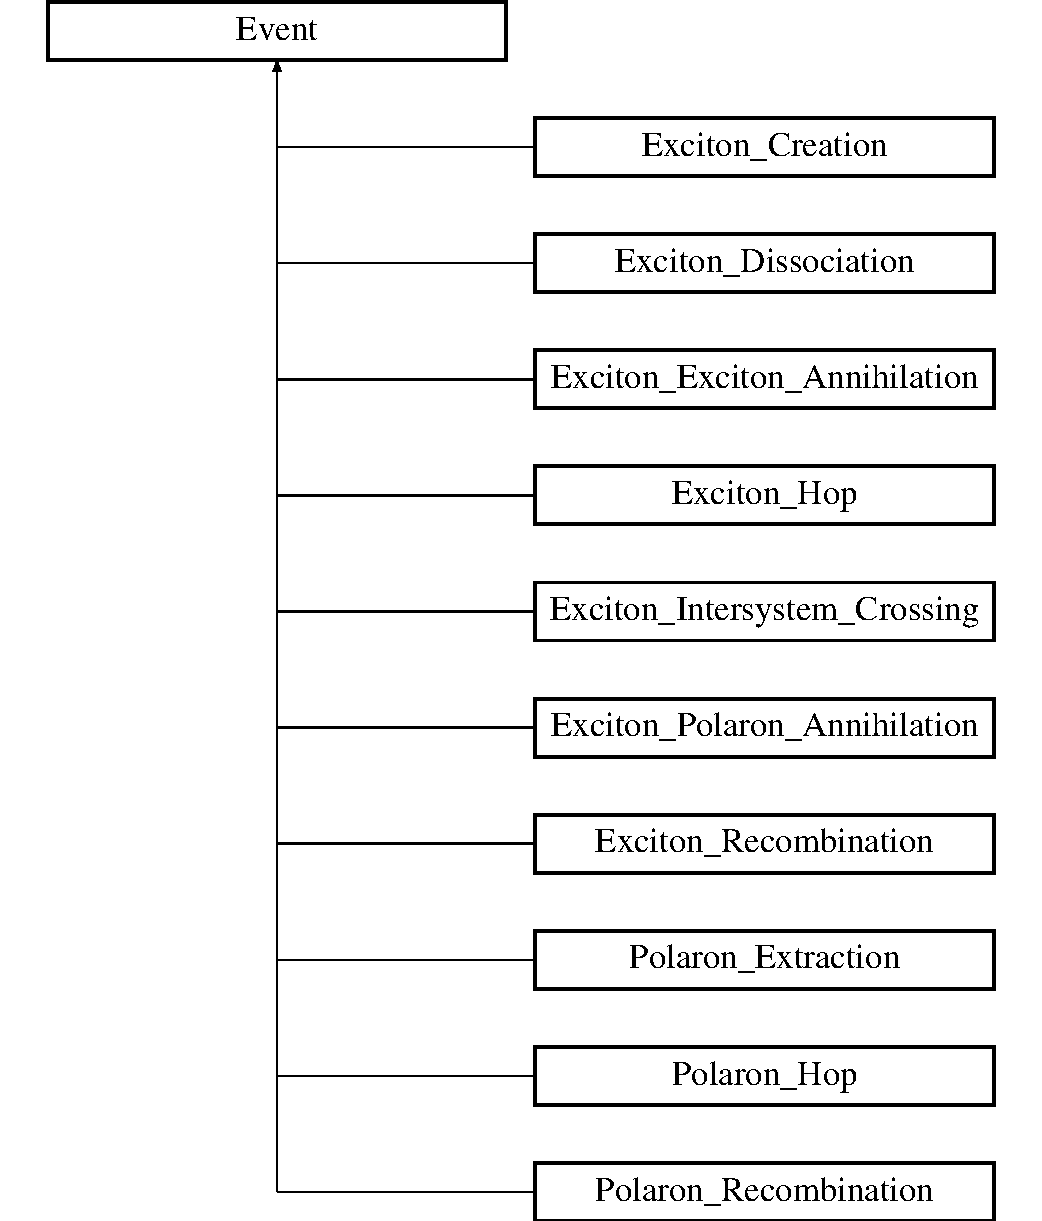
\includegraphics[height=11.000000cm]{class_event}
\end{center}
\end{figure}
\subsection*{Public Member Functions}
\begin{DoxyCompactItemize}
\item 
\mbox{\Hypertarget{class_event_a7704ec01ce91e673885792054214b3d2}\label{class_event_a7704ec01ce91e673885792054214b3d2}} 
virtual \hyperlink{class_event_a7704ec01ce91e673885792054214b3d2}{$\sim$\+Event} ()
\begin{DoxyCompactList}\small\item\em Default virtual destructor needed by the base class. \end{DoxyCompactList}\item 
\mbox{\Hypertarget{class_event_a5a40dd4708297f7031e29b39e039ae10}\label{class_event_a5a40dd4708297f7031e29b39e039ae10}} 
\hyperlink{class_event_a5a40dd4708297f7031e29b39e039ae10}{Event} ()
\begin{DoxyCompactList}\small\item\em Default constructor that creates an empty \hyperlink{class_event}{Event} object. \end{DoxyCompactList}\item 
void \hyperlink{class_event_a14b3f90f4b4d72ab1d0bf70f9b4cc907}{calculate\+Execution\+Time} (const double rate, \hyperlink{class_simulation}{Simulation} $\ast$sim\+\_\+ptr)
\begin{DoxyCompactList}\small\item\em Calculates and sets the execution time of the event. \end{DoxyCompactList}\item 
\hyperlink{struct_coords}{Coords} \hyperlink{class_event_a6b4287971afaca8211f91f361ef55997}{get\+Dest\+Coords} () const
\begin{DoxyCompactList}\small\item\em Gets the coordinates of the event destination site. \end{DoxyCompactList}\item 
virtual std\+::string \hyperlink{class_event_a8c38a406d844d05eac1ef007bad2487f}{get\+Name} () const
\begin{DoxyCompactList}\small\item\em Gets the name of event class. \end{DoxyCompactList}\item 
\hyperlink{class_object}{Object} $\ast$ \hyperlink{class_event_a5317d42bb07d0e75bec0c13bd9bf6de8}{get\+Object\+Ptr} () const
\begin{DoxyCompactList}\small\item\em Gets a pointer to the \hyperlink{class_object}{Object} object that is designated as the subject of the event. \end{DoxyCompactList}\item 
\hyperlink{class_object}{Object} $\ast$ \hyperlink{class_event_ab86f724c3c894faa1d6ccca78c357d24}{get\+Object\+Target\+Ptr} () const
\begin{DoxyCompactList}\small\item\em Gets a pointer to the \hyperlink{class_object}{Object} object that is designated as the target of the event. \end{DoxyCompactList}\item 
double \hyperlink{class_event_a65550d982cdf85d993658cd7070c960c}{get\+Execution\+Time} () const
\begin{DoxyCompactList}\small\item\em Gets the currently planned execution time of the event. \end{DoxyCompactList}\item 
void \hyperlink{class_event_a166ae40f2bf26c1e08097697ca76c884}{set\+Dest\+Coords} (const \hyperlink{struct_coords}{Coords} \&coords)
\begin{DoxyCompactList}\small\item\em Sets the desination coordinates of the event. \end{DoxyCompactList}\item 
bool \hyperlink{class_event_af4282af20bd5b3940ba75c23e6032f18}{set\+Execution\+Time} (const double time)
\begin{DoxyCompactList}\small\item\em Sets the execution time of the event. \end{DoxyCompactList}\item 
void \hyperlink{class_event_a078cadde679fc042486ef065a097c7af}{set\+Object\+Ptr} (\hyperlink{class_object}{Object} $\ast$input\+\_\+ptr)
\begin{DoxyCompactList}\small\item\em Sets the pointer to the \hyperlink{class_object}{Object} object that is designated as the subject of the event. \end{DoxyCompactList}\item 
void \hyperlink{class_event_a2e868dc951b6fec86703dcd7776680e0}{set\+Object\+Target\+Ptr} (\hyperlink{class_object}{Object} $\ast$input\+\_\+ptr)
\begin{DoxyCompactList}\small\item\em Sets the pointer to the \hyperlink{class_object}{Object} object that is designated as the target of the event. \end{DoxyCompactList}\end{DoxyCompactItemize}


\subsection{Detailed Description}
This base class contains the basic properties of a K\+MC simulation event and the functions needed to interact with it. 

This base class is designed to work with the \hyperlink{class_simulation}{Simulation} class to construct a K\+MC simulation. This base class is intended to be extended to create classes that represent specific types of events. \begin{DoxyCopyright}{Copyright}
M\+IT License. For more information, see the L\+I\+C\+E\+N\+SE file that accompanies this software package. 
\end{DoxyCopyright}
\begin{DoxyAuthor}{Author}
Michael C. Heiber 
\end{DoxyAuthor}
\begin{DoxyDate}{Date}
2017 
\end{DoxyDate}


\subsection{Member Function Documentation}
\mbox{\Hypertarget{class_event_a14b3f90f4b4d72ab1d0bf70f9b4cc907}\label{class_event_a14b3f90f4b4d72ab1d0bf70f9b4cc907}} 
\index{Event@{Event}!calculate\+Execution\+Time@{calculate\+Execution\+Time}}
\index{calculate\+Execution\+Time@{calculate\+Execution\+Time}!Event@{Event}}
\subsubsection{\texorpdfstring{calculate\+Execution\+Time()}{calculateExecutionTime()}}
{\footnotesize\ttfamily void Event\+::calculate\+Execution\+Time (\begin{DoxyParamCaption}\item[{const double}]{rate,  }\item[{\hyperlink{class_simulation}{Simulation} $\ast$}]{sim\+\_\+ptr }\end{DoxyParamCaption})}



Calculates and sets the execution time of the event. 

The function accesses the random number generator and current simulation time from the \hyperlink{class_simulation}{Simulation} object in order to calculate the execution time. When creating a new derived event class, one will often write a new calculate\+Execution\+Time function that contains additional factors needed to calculate the rate. This base class function can then be called within the new function to calculate the final execution time. 
\begin{DoxyParams}{Parameters}
{\em rate} & is the rate of the process represented by the event in units of 1/s. \\
\hline
{\em sim\+\_\+ptr} & is a pointer to a \hyperlink{class_simulation}{Simulation} object. \\
\hline
\end{DoxyParams}
\mbox{\Hypertarget{class_event_a6b4287971afaca8211f91f361ef55997}\label{class_event_a6b4287971afaca8211f91f361ef55997}} 
\index{Event@{Event}!get\+Dest\+Coords@{get\+Dest\+Coords}}
\index{get\+Dest\+Coords@{get\+Dest\+Coords}!Event@{Event}}
\subsubsection{\texorpdfstring{get\+Dest\+Coords()}{getDestCoords()}}
{\footnotesize\ttfamily \hyperlink{struct_coords}{Coords} Event\+::get\+Dest\+Coords (\begin{DoxyParamCaption}{ }\end{DoxyParamCaption}) const}



Gets the coordinates of the event destination site. 

\begin{DoxyWarning}{Warning}
Some events may not have a destination site determined until execution and will thus not have a valid set of coordinates defined. 
\end{DoxyWarning}
\begin{DoxyReturn}{Returns}
The coordinates of the destination site if valid coordinates have been set. 

The coordinates (-\/1,-\/1,-\/1) if no valid destination site has been set. 
\end{DoxyReturn}
\mbox{\Hypertarget{class_event_a65550d982cdf85d993658cd7070c960c}\label{class_event_a65550d982cdf85d993658cd7070c960c}} 
\index{Event@{Event}!get\+Execution\+Time@{get\+Execution\+Time}}
\index{get\+Execution\+Time@{get\+Execution\+Time}!Event@{Event}}
\subsubsection{\texorpdfstring{get\+Execution\+Time()}{getExecutionTime()}}
{\footnotesize\ttfamily double Event\+::get\+Execution\+Time (\begin{DoxyParamCaption}{ }\end{DoxyParamCaption}) const}



Gets the currently planned execution time of the event. 

\begin{DoxyReturn}{Returns}
0 if the event execution time has not yet been calculated. 

the currently planned execution time of the event in units of seconds. 
\end{DoxyReturn}
\mbox{\Hypertarget{class_event_a8c38a406d844d05eac1ef007bad2487f}\label{class_event_a8c38a406d844d05eac1ef007bad2487f}} 
\index{Event@{Event}!get\+Name@{get\+Name}}
\index{get\+Name@{get\+Name}!Event@{Event}}
\subsubsection{\texorpdfstring{get\+Name()}{getName()}}
{\footnotesize\ttfamily string Event\+::get\+Name (\begin{DoxyParamCaption}{ }\end{DoxyParamCaption}) const\hspace{0.3cm}{\ttfamily [virtual]}}



Gets the name of event class. 

\begin{DoxyReturn}{Returns}
\char`\"{}\+Event\char`\"{} when called on the base class. 
\end{DoxyReturn}


Reimplemented in \hyperlink{class_exciton___polaron___annihilation_aea3ae0f18ba7743d2183c2c5fbf4d4c4}{Exciton\+\_\+\+Polaron\+\_\+\+Annihilation}, \hyperlink{class_exciton___exciton___annihilation_a7027d2bee875a346e4c7ec4f07c55816}{Exciton\+\_\+\+Exciton\+\_\+\+Annihilation}, \hyperlink{class_exciton___intersystem___crossing_aa9a743fa3ab0ebc24abeaacef0590488}{Exciton\+\_\+\+Intersystem\+\_\+\+Crossing}, \hyperlink{class_exciton___dissociation_a1cfdbcfa3930666e0fddea28cc18ac9e}{Exciton\+\_\+\+Dissociation}, \hyperlink{class_polaron___extraction_a30cc8c9489f69e24feda42c035adc9cf}{Polaron\+\_\+\+Extraction}, \hyperlink{class_polaron___recombination_a0075250a377d6fccb8f64e4d173c9041}{Polaron\+\_\+\+Recombination}, \hyperlink{class_exciton___recombination_ac4142920b4692cdc107b0e877c7c8310}{Exciton\+\_\+\+Recombination}, \hyperlink{class_exciton___hop_a8e08c3992b06fa0efe7db438a381445b}{Exciton\+\_\+\+Hop}, \hyperlink{class_polaron___hop_adbb1a3f86bd6a2dd21849bfec5598d70}{Polaron\+\_\+\+Hop}, and \hyperlink{class_exciton___creation_aba92afc6c2aa48ce15c59c9e7310c636}{Exciton\+\_\+\+Creation}.

\mbox{\Hypertarget{class_event_a5317d42bb07d0e75bec0c13bd9bf6de8}\label{class_event_a5317d42bb07d0e75bec0c13bd9bf6de8}} 
\index{Event@{Event}!get\+Object\+Ptr@{get\+Object\+Ptr}}
\index{get\+Object\+Ptr@{get\+Object\+Ptr}!Event@{Event}}
\subsubsection{\texorpdfstring{get\+Object\+Ptr()}{getObjectPtr()}}
{\footnotesize\ttfamily \hyperlink{class_object}{Object} $\ast$ Event\+::get\+Object\+Ptr (\begin{DoxyParamCaption}{ }\end{DoxyParamCaption}) const}



Gets a pointer to the \hyperlink{class_object}{Object} object that is designated as the subject of the event. 

\begin{DoxyWarning}{Warning}
Some events may not operate on an object and will thus not have a subject object associated with them. 
\end{DoxyWarning}
\begin{DoxyReturn}{Returns}
nullptr if a valid \hyperlink{class_object}{Object} object has not been designated as the subject of the event. 
\end{DoxyReturn}
\mbox{\Hypertarget{class_event_ab86f724c3c894faa1d6ccca78c357d24}\label{class_event_ab86f724c3c894faa1d6ccca78c357d24}} 
\index{Event@{Event}!get\+Object\+Target\+Ptr@{get\+Object\+Target\+Ptr}}
\index{get\+Object\+Target\+Ptr@{get\+Object\+Target\+Ptr}!Event@{Event}}
\subsubsection{\texorpdfstring{get\+Object\+Target\+Ptr()}{getObjectTargetPtr()}}
{\footnotesize\ttfamily \hyperlink{class_object}{Object} $\ast$ Event\+::get\+Object\+Target\+Ptr (\begin{DoxyParamCaption}{ }\end{DoxyParamCaption}) const}



Gets a pointer to the \hyperlink{class_object}{Object} object that is designated as the target of the event. 

\begin{DoxyWarning}{Warning}
Some events may not have a valid target object assigned. A target object will only be defined when the event represent a reaction of some type between two objects. 
\end{DoxyWarning}
\begin{DoxyReturn}{Returns}
nullptr if a valid \hyperlink{class_object}{Object} object has not been designated as the target of the event. 
\end{DoxyReturn}
\mbox{\Hypertarget{class_event_a166ae40f2bf26c1e08097697ca76c884}\label{class_event_a166ae40f2bf26c1e08097697ca76c884}} 
\index{Event@{Event}!set\+Dest\+Coords@{set\+Dest\+Coords}}
\index{set\+Dest\+Coords@{set\+Dest\+Coords}!Event@{Event}}
\subsubsection{\texorpdfstring{set\+Dest\+Coords()}{setDestCoords()}}
{\footnotesize\ttfamily void Event\+::set\+Dest\+Coords (\begin{DoxyParamCaption}\item[{const \hyperlink{struct_coords}{Coords} \&}]{coords }\end{DoxyParamCaption})}



Sets the desination coordinates of the event. 


\begin{DoxyParams}{Parameters}
{\em coords} & is the \hyperlink{struct_coords}{Coords} struct that designates the input coordinates. \\
\hline
\end{DoxyParams}
\mbox{\Hypertarget{class_event_af4282af20bd5b3940ba75c23e6032f18}\label{class_event_af4282af20bd5b3940ba75c23e6032f18}} 
\index{Event@{Event}!set\+Execution\+Time@{set\+Execution\+Time}}
\index{set\+Execution\+Time@{set\+Execution\+Time}!Event@{Event}}
\subsubsection{\texorpdfstring{set\+Execution\+Time()}{setExecutionTime()}}
{\footnotesize\ttfamily bool Event\+::set\+Execution\+Time (\begin{DoxyParamCaption}\item[{const double}]{time }\end{DoxyParamCaption})}



Sets the execution time of the event. 


\begin{DoxyParams}{Parameters}
{\em time} & is the input time. \\
\hline
\end{DoxyParams}
\begin{DoxyReturn}{Returns}
true if the input time non-\/negative. 

false if the input is negative to indicate an error. 
\end{DoxyReturn}
\mbox{\Hypertarget{class_event_a078cadde679fc042486ef065a097c7af}\label{class_event_a078cadde679fc042486ef065a097c7af}} 
\index{Event@{Event}!set\+Object\+Ptr@{set\+Object\+Ptr}}
\index{set\+Object\+Ptr@{set\+Object\+Ptr}!Event@{Event}}
\subsubsection{\texorpdfstring{set\+Object\+Ptr()}{setObjectPtr()}}
{\footnotesize\ttfamily void Event\+::set\+Object\+Ptr (\begin{DoxyParamCaption}\item[{\hyperlink{class_object}{Object} $\ast$}]{input\+\_\+ptr }\end{DoxyParamCaption})}



Sets the pointer to the \hyperlink{class_object}{Object} object that is designated as the subject of the event. 


\begin{DoxyParams}{Parameters}
{\em input\+\_\+ptr} & is the input \hyperlink{class_object}{Object} pointer. \\
\hline
\end{DoxyParams}
\mbox{\Hypertarget{class_event_a2e868dc951b6fec86703dcd7776680e0}\label{class_event_a2e868dc951b6fec86703dcd7776680e0}} 
\index{Event@{Event}!set\+Object\+Target\+Ptr@{set\+Object\+Target\+Ptr}}
\index{set\+Object\+Target\+Ptr@{set\+Object\+Target\+Ptr}!Event@{Event}}
\subsubsection{\texorpdfstring{set\+Object\+Target\+Ptr()}{setObjectTargetPtr()}}
{\footnotesize\ttfamily void Event\+::set\+Object\+Target\+Ptr (\begin{DoxyParamCaption}\item[{\hyperlink{class_object}{Object} $\ast$}]{input\+\_\+ptr }\end{DoxyParamCaption})}



Sets the pointer to the \hyperlink{class_object}{Object} object that is designated as the target of the event. 


\begin{DoxyParams}{Parameters}
{\em input\+\_\+ptr} & is the input \hyperlink{class_object}{Object} pointer. \\
\hline
\end{DoxyParams}


The documentation for this class was generated from the following files\+:\begin{DoxyCompactItemize}
\item 
K\+M\+C\+\_\+\+Lattice/Event.\+h\item 
K\+M\+C\+\_\+\+Lattice/Event.\+cpp\end{DoxyCompactItemize}

\hypertarget{class_exciton}{}\section{Exciton Class Reference}
\label{class_exciton}\index{Exciton@{Exciton}}
Inheritance diagram for Exciton\+:\begin{figure}[H]
\begin{center}
\leavevmode
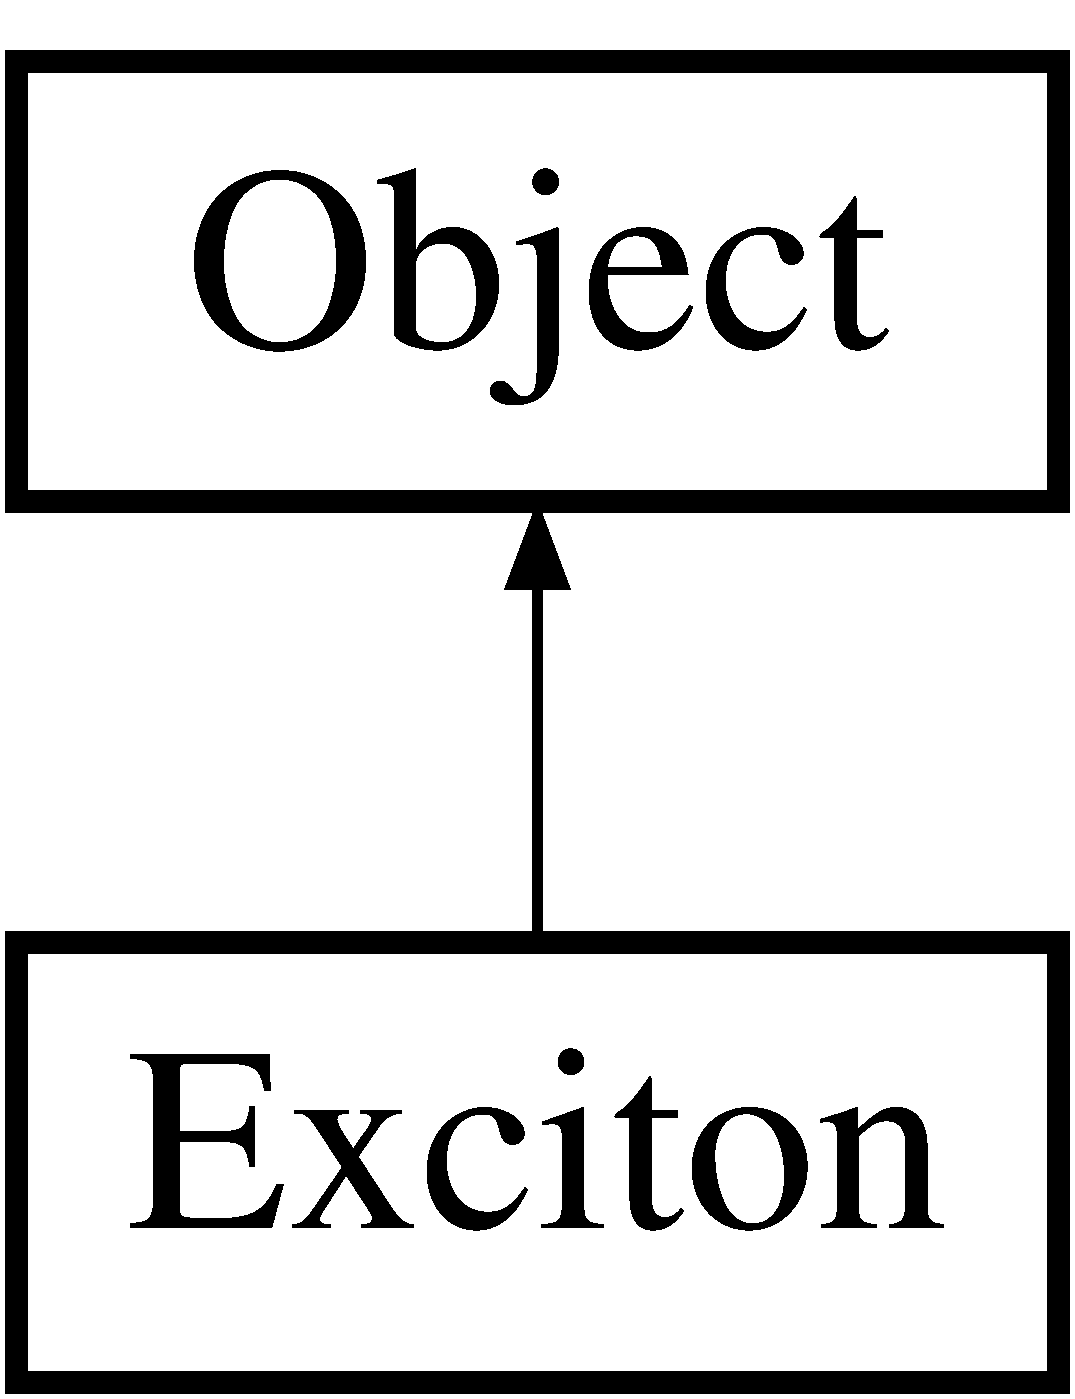
\includegraphics[height=2.000000cm]{class_exciton}
\end{center}
\end{figure}
\subsection*{Public Member Functions}
\begin{DoxyCompactItemize}
\item 
\mbox{\Hypertarget{class_exciton_a105a259c1235f22972cd25d811a750e7}\label{class_exciton_a105a259c1235f22972cd25d811a750e7}} 
{\bfseries Exciton} (const double time, const int tag\+\_\+num, const \hyperlink{struct_coords}{Coords} \&start\+\_\+coords)
\item 
\mbox{\Hypertarget{class_exciton_a85a7b8561f6e294593679e53dd3b91a9}\label{class_exciton_a85a7b8561f6e294593679e53dd3b91a9}} 
void {\bfseries flip\+Spin} ()
\item 
std\+::string \hyperlink{class_exciton_a4db43bd7ca4136e35f9a50b2a5854728}{get\+Name} () const
\begin{DoxyCompactList}\small\item\em Gets the name of the \hyperlink{class_object}{Object} class. \end{DoxyCompactList}\item 
\mbox{\Hypertarget{class_exciton_a91cb4c59b7e7a7fb756aae4c4109dba3}\label{class_exciton_a91cb4c59b7e7a7fb756aae4c4109dba3}} 
bool {\bfseries get\+Spin} () const
\item 
\mbox{\Hypertarget{class_exciton_ac4c632e42b902209de783fde48d74269}\label{class_exciton_ac4c632e42b902209de783fde48d74269}} 
void {\bfseries set\+Spin} (bool spin\+\_\+state)
\end{DoxyCompactItemize}
\subsection*{Static Public Attributes}
\begin{DoxyCompactItemize}
\item 
\mbox{\Hypertarget{class_exciton_a455155f7d0a91a1ada55b64cf25b3405}\label{class_exciton_a455155f7d0a91a1ada55b64cf25b3405}} 
static const std\+::string {\bfseries name} = \char`\"{}Exciton\char`\"{}
\end{DoxyCompactItemize}


\subsection{Member Function Documentation}
\mbox{\Hypertarget{class_exciton_a4db43bd7ca4136e35f9a50b2a5854728}\label{class_exciton_a4db43bd7ca4136e35f9a50b2a5854728}} 
\index{Exciton@{Exciton}!get\+Name@{get\+Name}}
\index{get\+Name@{get\+Name}!Exciton@{Exciton}}
\subsubsection{\texorpdfstring{get\+Name()}{getName()}}
{\footnotesize\ttfamily std\+::string Exciton\+::get\+Name (\begin{DoxyParamCaption}{ }\end{DoxyParamCaption}) const\hspace{0.3cm}{\ttfamily [inline]}, {\ttfamily [virtual]}}



Gets the name of the \hyperlink{class_object}{Object} class. 

\begin{DoxyReturn}{Returns}
\char`\"{}\+Object\char`\"{} when called on the base class. 
\end{DoxyReturn}


Reimplemented from \hyperlink{class_object_ade517616d51cd9ab581ec5afeb37b313}{Object}.



The documentation for this class was generated from the following files\+:\begin{DoxyCompactItemize}
\item 
Exciton.\+h\item 
Exciton.\+cpp\end{DoxyCompactItemize}

\hypertarget{class_exciton___creation}{}\section{Exciton\+\_\+\+Creation Class Reference}
\label{class_exciton___creation}\index{Exciton\+\_\+\+Creation@{Exciton\+\_\+\+Creation}}
Inheritance diagram for Exciton\+\_\+\+Creation\+:\begin{figure}[H]
\begin{center}
\leavevmode
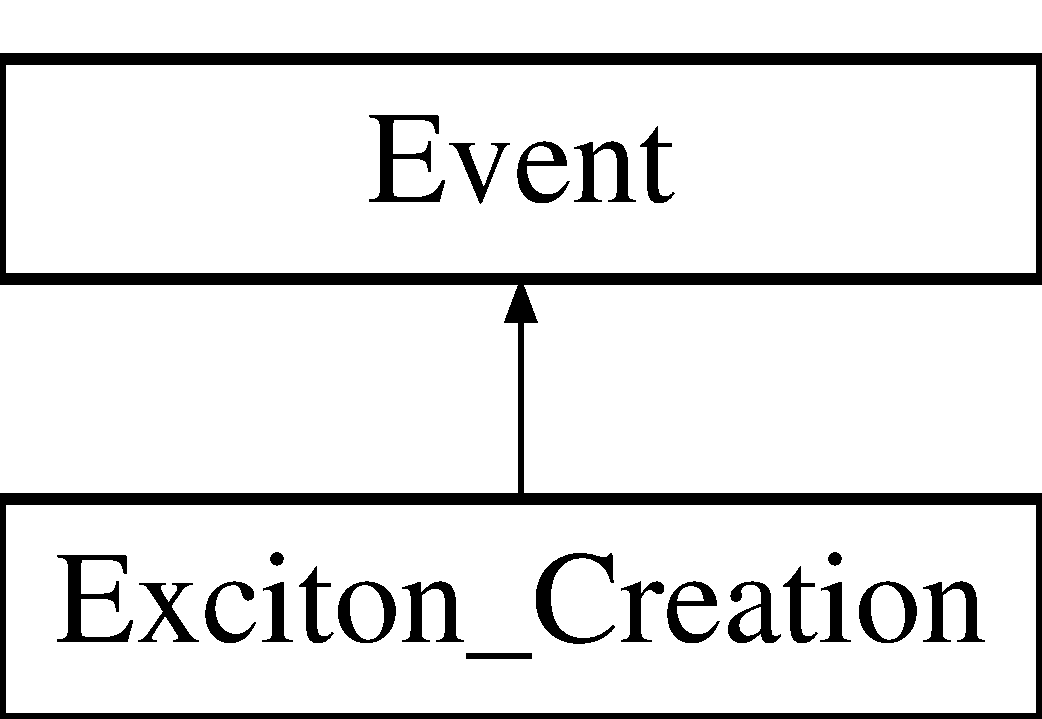
\includegraphics[height=2.000000cm]{class_exciton___creation}
\end{center}
\end{figure}
\subsection*{Public Member Functions}
\begin{DoxyCompactItemize}
\item 
std\+::string \hyperlink{class_exciton___creation_aba92afc6c2aa48ce15c59c9e7310c636}{get\+Name} () const
\begin{DoxyCompactList}\small\item\em Gets the name of event class. \end{DoxyCompactList}\end{DoxyCompactItemize}
\subsection*{Static Public Attributes}
\begin{DoxyCompactItemize}
\item 
\mbox{\Hypertarget{class_exciton___creation_a4e72153bdee28c070e978b871eac7c9c}\label{class_exciton___creation_a4e72153bdee28c070e978b871eac7c9c}} 
static const std\+::string {\bfseries name} = \char`\"{}Exciton Creation\char`\"{}
\end{DoxyCompactItemize}


\subsection{Member Function Documentation}
\mbox{\Hypertarget{class_exciton___creation_aba92afc6c2aa48ce15c59c9e7310c636}\label{class_exciton___creation_aba92afc6c2aa48ce15c59c9e7310c636}} 
\index{Exciton\+\_\+\+Creation@{Exciton\+\_\+\+Creation}!get\+Name@{get\+Name}}
\index{get\+Name@{get\+Name}!Exciton\+\_\+\+Creation@{Exciton\+\_\+\+Creation}}
\subsubsection{\texorpdfstring{get\+Name()}{getName()}}
{\footnotesize\ttfamily std\+::string Exciton\+\_\+\+Creation\+::get\+Name (\begin{DoxyParamCaption}{ }\end{DoxyParamCaption}) const\hspace{0.3cm}{\ttfamily [inline]}, {\ttfamily [virtual]}}



Gets the name of event class. 

\begin{DoxyReturn}{Returns}
\char`\"{}\+Event\char`\"{} when called on the base class. 
\end{DoxyReturn}


Reimplemented from \hyperlink{class_event_a8c38a406d844d05eac1ef007bad2487f}{Event}.



The documentation for this class was generated from the following files\+:\begin{DoxyCompactItemize}
\item 
Exciton.\+h\item 
Exciton.\+cpp\end{DoxyCompactItemize}

\hypertarget{class_exciton___dissociation}{}\section{Exciton\+\_\+\+Dissociation Class Reference}
\label{class_exciton___dissociation}\index{Exciton\+\_\+\+Dissociation@{Exciton\+\_\+\+Dissociation}}
Inheritance diagram for Exciton\+\_\+\+Dissociation\+:\begin{figure}[H]
\begin{center}
\leavevmode
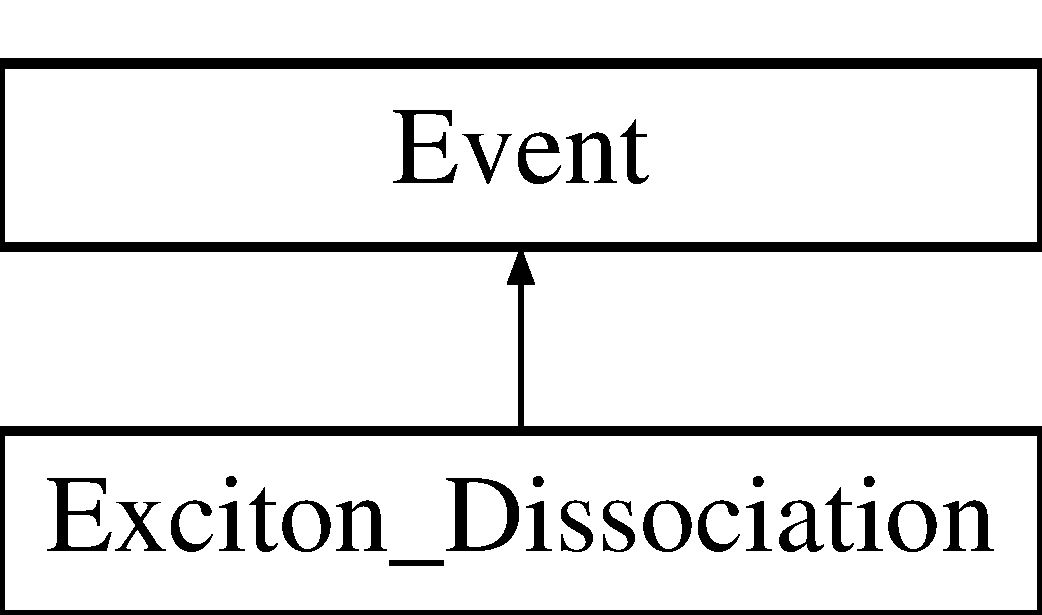
\includegraphics[height=2.000000cm]{class_exciton___dissociation}
\end{center}
\end{figure}
\subsection*{Public Member Functions}
\begin{DoxyCompactItemize}
\item 
\mbox{\Hypertarget{class_exciton___dissociation_a2da846b02c20a7c070567de92762d53b}\label{class_exciton___dissociation_a2da846b02c20a7c070567de92762d53b}} 
void {\bfseries calculate\+Execution\+Time} (const double prefactor, const double localization, const double distance, const double E\+\_\+delta, \hyperlink{class_simulation}{Simulation} $\ast$sim\+\_\+ptr)
\item 
\mbox{\Hypertarget{class_exciton___dissociation_a8637e01b4532ba5442ded098883b64a0}\label{class_exciton___dissociation_a8637e01b4532ba5442ded098883b64a0}} 
void {\bfseries calculate\+Execution\+Time} (const double prefactor, const double localization, const double distance, const double E\+\_\+delta, const double reorganization, \hyperlink{class_simulation}{Simulation} $\ast$sim\+\_\+ptr)
\item 
std\+::string \hyperlink{class_exciton___dissociation_a1cfdbcfa3930666e0fddea28cc18ac9e}{get\+Name} () const
\begin{DoxyCompactList}\small\item\em Gets the name of event class. \end{DoxyCompactList}\end{DoxyCompactItemize}
\subsection*{Static Public Attributes}
\begin{DoxyCompactItemize}
\item 
\mbox{\Hypertarget{class_exciton___dissociation_a16a06165fe1c2468850b2d05243b24cd}\label{class_exciton___dissociation_a16a06165fe1c2468850b2d05243b24cd}} 
static const std\+::string {\bfseries name} = \char`\"{}Exciton Dissociation\char`\"{}
\end{DoxyCompactItemize}


\subsection{Member Function Documentation}
\mbox{\Hypertarget{class_exciton___dissociation_a1cfdbcfa3930666e0fddea28cc18ac9e}\label{class_exciton___dissociation_a1cfdbcfa3930666e0fddea28cc18ac9e}} 
\index{Exciton\+\_\+\+Dissociation@{Exciton\+\_\+\+Dissociation}!get\+Name@{get\+Name}}
\index{get\+Name@{get\+Name}!Exciton\+\_\+\+Dissociation@{Exciton\+\_\+\+Dissociation}}
\subsubsection{\texorpdfstring{get\+Name()}{getName()}}
{\footnotesize\ttfamily std\+::string Exciton\+\_\+\+Dissociation\+::get\+Name (\begin{DoxyParamCaption}{ }\end{DoxyParamCaption}) const\hspace{0.3cm}{\ttfamily [inline]}, {\ttfamily [virtual]}}



Gets the name of event class. 

\begin{DoxyReturn}{Returns}
\char`\"{}\+Event\char`\"{} when called on the base class. 
\end{DoxyReturn}


Reimplemented from \hyperlink{class_event_a8c38a406d844d05eac1ef007bad2487f}{Event}.



The documentation for this class was generated from the following files\+:\begin{DoxyCompactItemize}
\item 
Exciton.\+h\item 
Exciton.\+cpp\end{DoxyCompactItemize}

\hypertarget{class_exciton___exciton___annihilation}{}\section{Exciton\+\_\+\+Exciton\+\_\+\+Annihilation Class Reference}
\label{class_exciton___exciton___annihilation}\index{Exciton\+\_\+\+Exciton\+\_\+\+Annihilation@{Exciton\+\_\+\+Exciton\+\_\+\+Annihilation}}
Inheritance diagram for Exciton\+\_\+\+Exciton\+\_\+\+Annihilation\+:\begin{figure}[H]
\begin{center}
\leavevmode
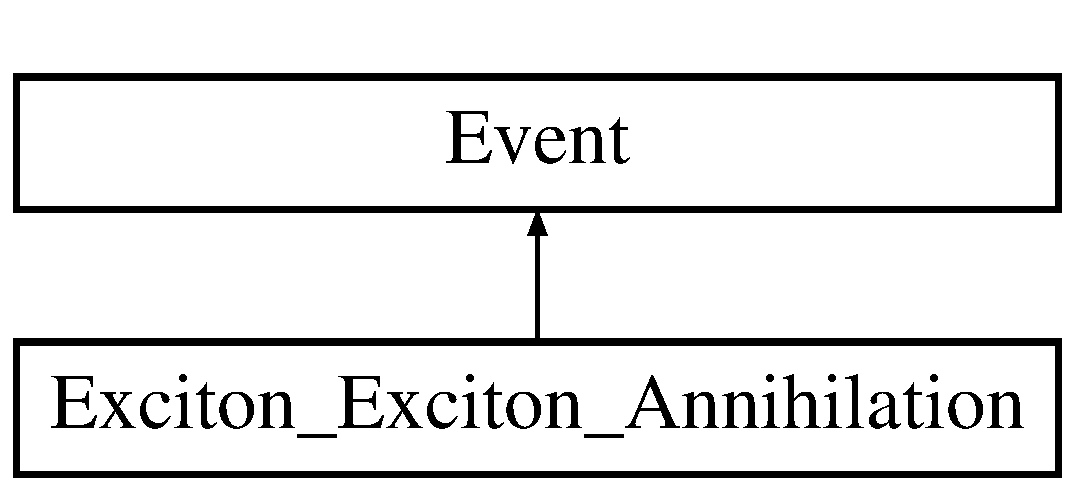
\includegraphics[height=2.000000cm]{class_exciton___exciton___annihilation}
\end{center}
\end{figure}
\subsection*{Public Member Functions}
\begin{DoxyCompactItemize}
\item 
\mbox{\Hypertarget{class_exciton___exciton___annihilation_a46aa32935c16084a6cea854d4350f413}\label{class_exciton___exciton___annihilation_a46aa32935c16084a6cea854d4350f413}} 
void {\bfseries calculate\+Execution\+Time} (const double prefactor, const double distance, \hyperlink{class_simulation}{Simulation} $\ast$sim\+\_\+ptr)
\item 
\mbox{\Hypertarget{class_exciton___exciton___annihilation_a7b5546b124fb9dfda409e48b4f6bc885}\label{class_exciton___exciton___annihilation_a7b5546b124fb9dfda409e48b4f6bc885}} 
void {\bfseries calculate\+Execution\+Time} (const double prefactor, const double localization, const double distance, \hyperlink{class_simulation}{Simulation} $\ast$sim\+\_\+ptr)
\item 
std\+::string \hyperlink{class_exciton___exciton___annihilation_a7027d2bee875a346e4c7ec4f07c55816}{get\+Name} () const
\begin{DoxyCompactList}\small\item\em Gets the name of event class. \end{DoxyCompactList}\end{DoxyCompactItemize}
\subsection*{Static Public Attributes}
\begin{DoxyCompactItemize}
\item 
\mbox{\Hypertarget{class_exciton___exciton___annihilation_a8dee3797f6dc1c50276e06117bee82ac}\label{class_exciton___exciton___annihilation_a8dee3797f6dc1c50276e06117bee82ac}} 
static const std\+::string {\bfseries name} = \char`\"{}Exciton-\/\hyperlink{class_exciton}{Exciton} Annihilation\char`\"{}
\end{DoxyCompactItemize}


\subsection{Member Function Documentation}
\mbox{\Hypertarget{class_exciton___exciton___annihilation_a7027d2bee875a346e4c7ec4f07c55816}\label{class_exciton___exciton___annihilation_a7027d2bee875a346e4c7ec4f07c55816}} 
\index{Exciton\+\_\+\+Exciton\+\_\+\+Annihilation@{Exciton\+\_\+\+Exciton\+\_\+\+Annihilation}!get\+Name@{get\+Name}}
\index{get\+Name@{get\+Name}!Exciton\+\_\+\+Exciton\+\_\+\+Annihilation@{Exciton\+\_\+\+Exciton\+\_\+\+Annihilation}}
\subsubsection{\texorpdfstring{get\+Name()}{getName()}}
{\footnotesize\ttfamily std\+::string Exciton\+\_\+\+Exciton\+\_\+\+Annihilation\+::get\+Name (\begin{DoxyParamCaption}{ }\end{DoxyParamCaption}) const\hspace{0.3cm}{\ttfamily [inline]}, {\ttfamily [virtual]}}



Gets the name of event class. 

\begin{DoxyReturn}{Returns}
\char`\"{}\+Event\char`\"{} when called on the base class. 
\end{DoxyReturn}


Reimplemented from \hyperlink{class_event_a8c38a406d844d05eac1ef007bad2487f}{Event}.



The documentation for this class was generated from the following files\+:\begin{DoxyCompactItemize}
\item 
Exciton.\+h\item 
Exciton.\+cpp\end{DoxyCompactItemize}

\hypertarget{class_exciton___hop}{}\section{Exciton\+\_\+\+Hop Class Reference}
\label{class_exciton___hop}\index{Exciton\+\_\+\+Hop@{Exciton\+\_\+\+Hop}}
Inheritance diagram for Exciton\+\_\+\+Hop\+:\begin{figure}[H]
\begin{center}
\leavevmode
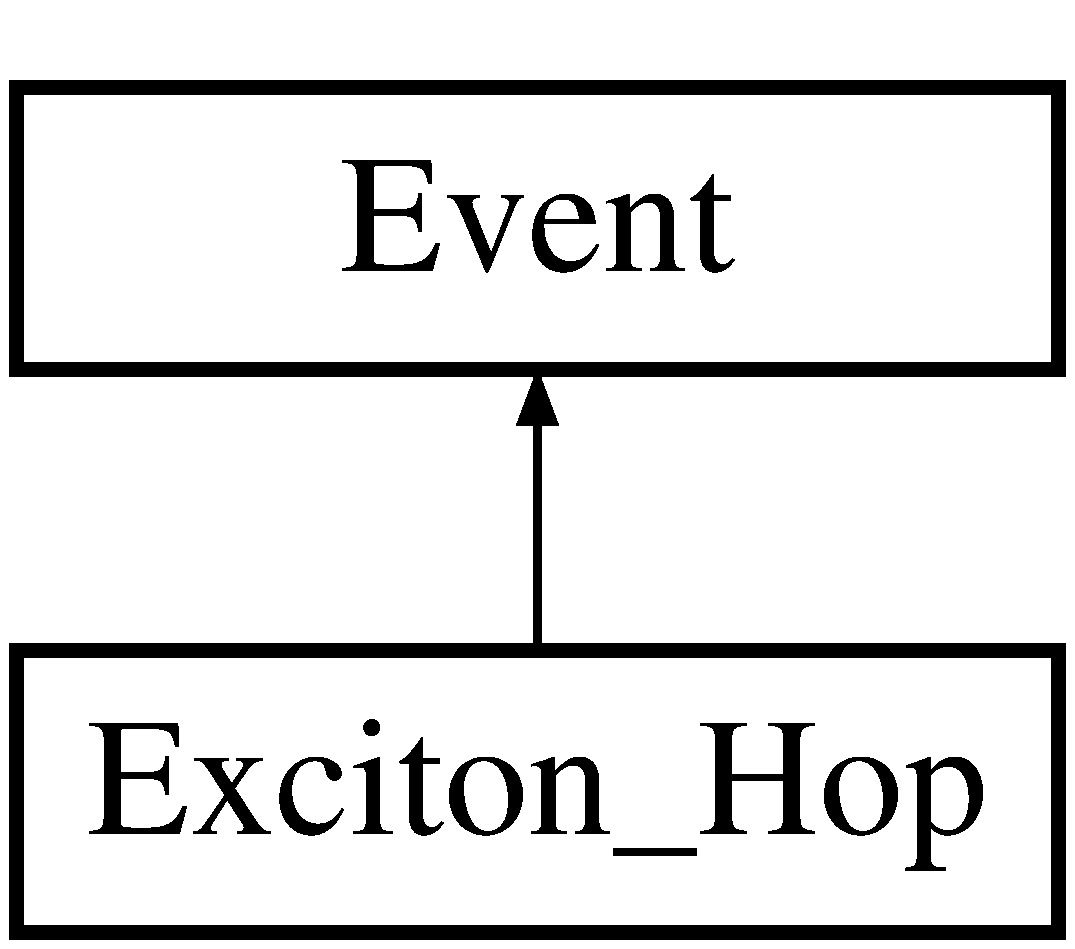
\includegraphics[height=2.000000cm]{class_exciton___hop}
\end{center}
\end{figure}
\subsection*{Public Member Functions}
\begin{DoxyCompactItemize}
\item 
\mbox{\Hypertarget{class_exciton___hop_a592dffe088b974fc5c6e12629c97b4df}\label{class_exciton___hop_a592dffe088b974fc5c6e12629c97b4df}} 
void {\bfseries calculate\+Execution\+Time} (const double prefactor, const double distance, const double E\+\_\+delta, \hyperlink{class_simulation}{Simulation} $\ast$sim\+\_\+ptr)
\item 
\mbox{\Hypertarget{class_exciton___hop_abcdc64e255936380a8437a048a81b75b}\label{class_exciton___hop_abcdc64e255936380a8437a048a81b75b}} 
void {\bfseries calculate\+Execution\+Time} (const double prefactor, const double localization, const double distance, const double E\+\_\+delta, \hyperlink{class_simulation}{Simulation} $\ast$sim\+\_\+ptr)
\item 
std\+::string \hyperlink{class_exciton___hop_a8e08c3992b06fa0efe7db438a381445b}{get\+Name} () const
\begin{DoxyCompactList}\small\item\em Gets the name of event class. \end{DoxyCompactList}\end{DoxyCompactItemize}
\subsection*{Static Public Attributes}
\begin{DoxyCompactItemize}
\item 
\mbox{\Hypertarget{class_exciton___hop_abdb3ad0035448cdb55215a4f641b2150}\label{class_exciton___hop_abdb3ad0035448cdb55215a4f641b2150}} 
static const std\+::string {\bfseries name} = \char`\"{}Exciton Hop\char`\"{}
\end{DoxyCompactItemize}


\subsection{Member Function Documentation}
\mbox{\Hypertarget{class_exciton___hop_a8e08c3992b06fa0efe7db438a381445b}\label{class_exciton___hop_a8e08c3992b06fa0efe7db438a381445b}} 
\index{Exciton\+\_\+\+Hop@{Exciton\+\_\+\+Hop}!get\+Name@{get\+Name}}
\index{get\+Name@{get\+Name}!Exciton\+\_\+\+Hop@{Exciton\+\_\+\+Hop}}
\subsubsection{\texorpdfstring{get\+Name()}{getName()}}
{\footnotesize\ttfamily std\+::string Exciton\+\_\+\+Hop\+::get\+Name (\begin{DoxyParamCaption}{ }\end{DoxyParamCaption}) const\hspace{0.3cm}{\ttfamily [inline]}, {\ttfamily [virtual]}}



Gets the name of event class. 

\begin{DoxyReturn}{Returns}
\char`\"{}\+Event\char`\"{} when called on the base class. 
\end{DoxyReturn}


Reimplemented from \hyperlink{class_event_a8c38a406d844d05eac1ef007bad2487f}{Event}.



The documentation for this class was generated from the following files\+:\begin{DoxyCompactItemize}
\item 
Exciton.\+h\item 
Exciton.\+cpp\end{DoxyCompactItemize}

\hypertarget{class_exciton___intersystem___crossing}{}\section{Exciton\+\_\+\+Intersystem\+\_\+\+Crossing Class Reference}
\label{class_exciton___intersystem___crossing}\index{Exciton\+\_\+\+Intersystem\+\_\+\+Crossing@{Exciton\+\_\+\+Intersystem\+\_\+\+Crossing}}
Inheritance diagram for Exciton\+\_\+\+Intersystem\+\_\+\+Crossing\+:\begin{figure}[H]
\begin{center}
\leavevmode
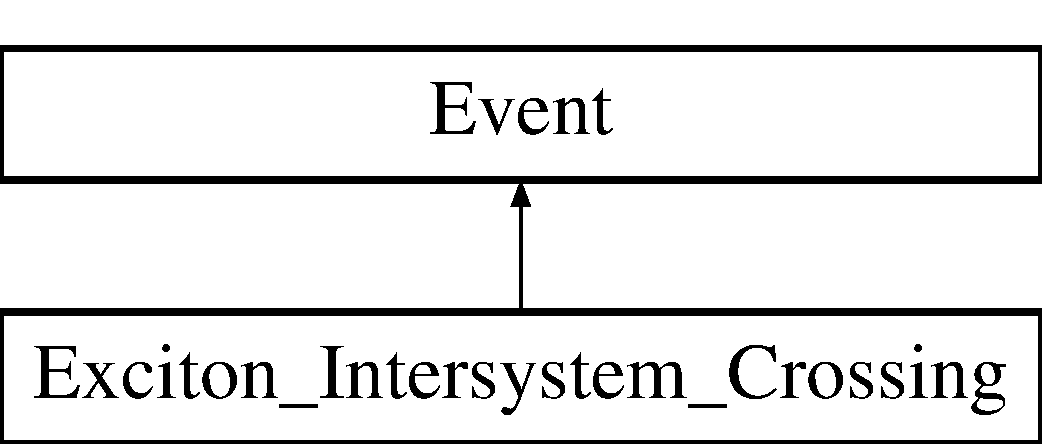
\includegraphics[height=2.000000cm]{class_exciton___intersystem___crossing}
\end{center}
\end{figure}
\subsection*{Public Member Functions}
\begin{DoxyCompactItemize}
\item 
\mbox{\Hypertarget{class_exciton___intersystem___crossing_a7c4cd9f72c1fde140678a8e9bce18d81}\label{class_exciton___intersystem___crossing_a7c4cd9f72c1fde140678a8e9bce18d81}} 
void {\bfseries calculate\+Execution\+Time} (const double prefactor, const double E\+\_\+delta, \hyperlink{class_simulation}{Simulation} $\ast$sim\+\_\+ptr)
\item 
std\+::string \hyperlink{class_exciton___intersystem___crossing_aa9a743fa3ab0ebc24abeaacef0590488}{get\+Name} () const
\begin{DoxyCompactList}\small\item\em Gets the name of event class. \end{DoxyCompactList}\end{DoxyCompactItemize}
\subsection*{Static Public Attributes}
\begin{DoxyCompactItemize}
\item 
\mbox{\Hypertarget{class_exciton___intersystem___crossing_a4c9578265b37f2ab24f1747de3a1f2a2}\label{class_exciton___intersystem___crossing_a4c9578265b37f2ab24f1747de3a1f2a2}} 
static const std\+::string {\bfseries name} = \char`\"{}Exciton Intersystem Crossing\char`\"{}
\end{DoxyCompactItemize}


\subsection{Member Function Documentation}
\mbox{\Hypertarget{class_exciton___intersystem___crossing_aa9a743fa3ab0ebc24abeaacef0590488}\label{class_exciton___intersystem___crossing_aa9a743fa3ab0ebc24abeaacef0590488}} 
\index{Exciton\+\_\+\+Intersystem\+\_\+\+Crossing@{Exciton\+\_\+\+Intersystem\+\_\+\+Crossing}!get\+Name@{get\+Name}}
\index{get\+Name@{get\+Name}!Exciton\+\_\+\+Intersystem\+\_\+\+Crossing@{Exciton\+\_\+\+Intersystem\+\_\+\+Crossing}}
\subsubsection{\texorpdfstring{get\+Name()}{getName()}}
{\footnotesize\ttfamily std\+::string Exciton\+\_\+\+Intersystem\+\_\+\+Crossing\+::get\+Name (\begin{DoxyParamCaption}{ }\end{DoxyParamCaption}) const\hspace{0.3cm}{\ttfamily [inline]}, {\ttfamily [virtual]}}



Gets the name of event class. 

\begin{DoxyReturn}{Returns}
\char`\"{}\+Event\char`\"{} when called on the base class. 
\end{DoxyReturn}


Reimplemented from \hyperlink{class_event_a8c38a406d844d05eac1ef007bad2487f}{Event}.



The documentation for this class was generated from the following files\+:\begin{DoxyCompactItemize}
\item 
Exciton.\+h\item 
Exciton.\+cpp\end{DoxyCompactItemize}

\hypertarget{class_exciton___polaron___annihilation}{}\section{Exciton\+\_\+\+Polaron\+\_\+\+Annihilation Class Reference}
\label{class_exciton___polaron___annihilation}\index{Exciton\+\_\+\+Polaron\+\_\+\+Annihilation@{Exciton\+\_\+\+Polaron\+\_\+\+Annihilation}}
Inheritance diagram for Exciton\+\_\+\+Polaron\+\_\+\+Annihilation\+:\begin{figure}[H]
\begin{center}
\leavevmode
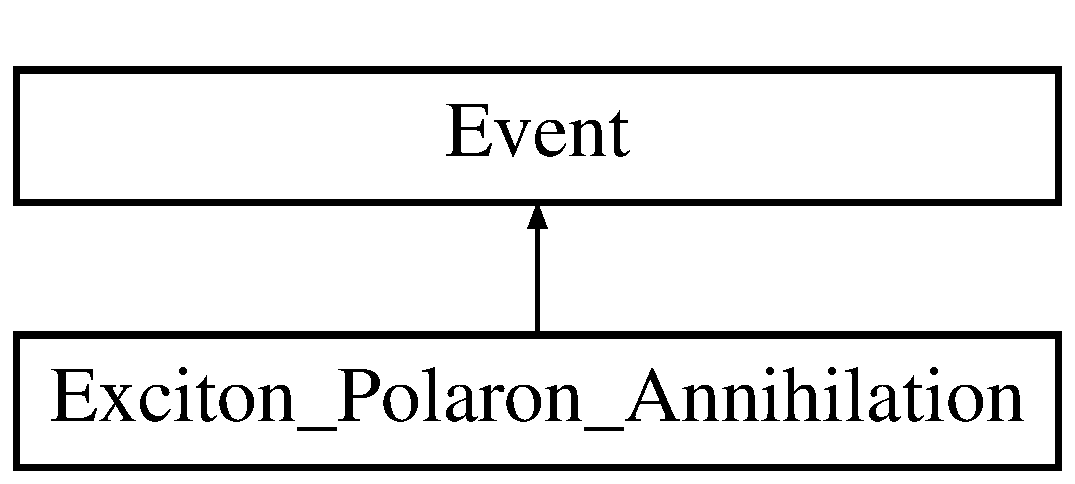
\includegraphics[height=2.000000cm]{class_exciton___polaron___annihilation}
\end{center}
\end{figure}
\subsection*{Public Member Functions}
\begin{DoxyCompactItemize}
\item 
\mbox{\Hypertarget{class_exciton___polaron___annihilation_a7206c9b930c1e1da35dc62e25c127e3c}\label{class_exciton___polaron___annihilation_a7206c9b930c1e1da35dc62e25c127e3c}} 
void {\bfseries calculate\+Execution\+Time} (const double prefactor, const double distance, \hyperlink{class_simulation}{Simulation} $\ast$sim\+\_\+ptr)
\item 
\mbox{\Hypertarget{class_exciton___polaron___annihilation_a5818e1cdc2e6fd3ba744826efd2c40bf}\label{class_exciton___polaron___annihilation_a5818e1cdc2e6fd3ba744826efd2c40bf}} 
void {\bfseries calculate\+Execution\+Time} (const double prefactor, const double localization, const double distance, \hyperlink{class_simulation}{Simulation} $\ast$sim\+\_\+ptr)
\item 
std\+::string \hyperlink{class_exciton___polaron___annihilation_aea3ae0f18ba7743d2183c2c5fbf4d4c4}{get\+Name} () const
\begin{DoxyCompactList}\small\item\em Gets the name of event class. \end{DoxyCompactList}\end{DoxyCompactItemize}
\subsection*{Static Public Attributes}
\begin{DoxyCompactItemize}
\item 
\mbox{\Hypertarget{class_exciton___polaron___annihilation_a49bc9251aed38c5a7249385d9bf93dc9}\label{class_exciton___polaron___annihilation_a49bc9251aed38c5a7249385d9bf93dc9}} 
static const std\+::string {\bfseries name} = \char`\"{}Exciton-\/\hyperlink{class_polaron}{Polaron} Annihilation\char`\"{}
\end{DoxyCompactItemize}


\subsection{Member Function Documentation}
\mbox{\Hypertarget{class_exciton___polaron___annihilation_aea3ae0f18ba7743d2183c2c5fbf4d4c4}\label{class_exciton___polaron___annihilation_aea3ae0f18ba7743d2183c2c5fbf4d4c4}} 
\index{Exciton\+\_\+\+Polaron\+\_\+\+Annihilation@{Exciton\+\_\+\+Polaron\+\_\+\+Annihilation}!get\+Name@{get\+Name}}
\index{get\+Name@{get\+Name}!Exciton\+\_\+\+Polaron\+\_\+\+Annihilation@{Exciton\+\_\+\+Polaron\+\_\+\+Annihilation}}
\subsubsection{\texorpdfstring{get\+Name()}{getName()}}
{\footnotesize\ttfamily std\+::string Exciton\+\_\+\+Polaron\+\_\+\+Annihilation\+::get\+Name (\begin{DoxyParamCaption}{ }\end{DoxyParamCaption}) const\hspace{0.3cm}{\ttfamily [inline]}, {\ttfamily [virtual]}}



Gets the name of event class. 

\begin{DoxyReturn}{Returns}
\char`\"{}\+Event\char`\"{} when called on the base class. 
\end{DoxyReturn}


Reimplemented from \hyperlink{class_event_a8c38a406d844d05eac1ef007bad2487f}{Event}.



The documentation for this class was generated from the following files\+:\begin{DoxyCompactItemize}
\item 
Exciton.\+h\item 
Exciton.\+cpp\end{DoxyCompactItemize}

\hypertarget{class_exciton___recombination}{}\section{Exciton\+\_\+\+Recombination Class Reference}
\label{class_exciton___recombination}\index{Exciton\+\_\+\+Recombination@{Exciton\+\_\+\+Recombination}}
Inheritance diagram for Exciton\+\_\+\+Recombination\+:\begin{figure}[H]
\begin{center}
\leavevmode
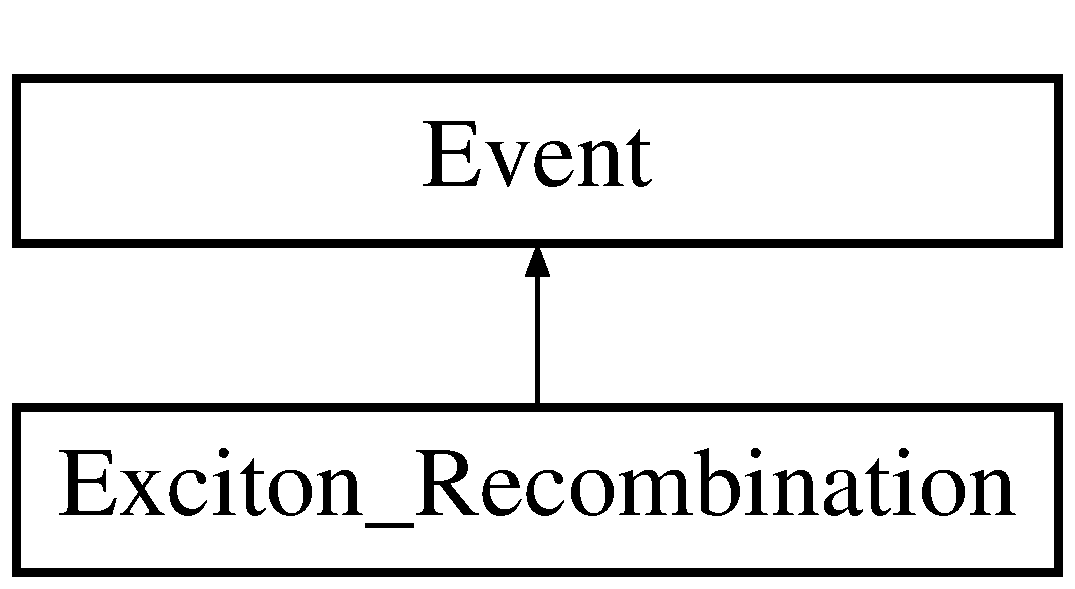
\includegraphics[height=2.000000cm]{class_exciton___recombination}
\end{center}
\end{figure}
\subsection*{Public Member Functions}
\begin{DoxyCompactItemize}
\item 
std\+::string \hyperlink{class_exciton___recombination_ac4142920b4692cdc107b0e877c7c8310}{get\+Name} () const
\begin{DoxyCompactList}\small\item\em Gets the name of event class. \end{DoxyCompactList}\end{DoxyCompactItemize}
\subsection*{Static Public Attributes}
\begin{DoxyCompactItemize}
\item 
\mbox{\Hypertarget{class_exciton___recombination_a601fbd52a90812058cb073fb57b1ad6f}\label{class_exciton___recombination_a601fbd52a90812058cb073fb57b1ad6f}} 
static const std\+::string {\bfseries name} = \char`\"{}Exciton Recombination\char`\"{}
\end{DoxyCompactItemize}


\subsection{Member Function Documentation}
\mbox{\Hypertarget{class_exciton___recombination_ac4142920b4692cdc107b0e877c7c8310}\label{class_exciton___recombination_ac4142920b4692cdc107b0e877c7c8310}} 
\index{Exciton\+\_\+\+Recombination@{Exciton\+\_\+\+Recombination}!get\+Name@{get\+Name}}
\index{get\+Name@{get\+Name}!Exciton\+\_\+\+Recombination@{Exciton\+\_\+\+Recombination}}
\subsubsection{\texorpdfstring{get\+Name()}{getName()}}
{\footnotesize\ttfamily std\+::string Exciton\+\_\+\+Recombination\+::get\+Name (\begin{DoxyParamCaption}{ }\end{DoxyParamCaption}) const\hspace{0.3cm}{\ttfamily [inline]}, {\ttfamily [virtual]}}



Gets the name of event class. 

\begin{DoxyReturn}{Returns}
\char`\"{}\+Event\char`\"{} when called on the base class. 
\end{DoxyReturn}


Reimplemented from \hyperlink{class_event_a8c38a406d844d05eac1ef007bad2487f}{Event}.



The documentation for this class was generated from the following files\+:\begin{DoxyCompactItemize}
\item 
Exciton.\+h\item 
Exciton.\+cpp\end{DoxyCompactItemize}

\hypertarget{class_lattice}{}\section{Lattice Class Reference}
\label{class_lattice}\index{Lattice@{Lattice}}


This class contains the properties of a three-\/dimensional lattice and the functions needed to interact with it.  




{\ttfamily \#include $<$Lattice.\+h$>$}

\subsection*{Public Member Functions}
\begin{DoxyCompactItemize}
\item 
\hyperlink{class_lattice_a70a5cebc3c0c5a0f609be0592e7cc117}{Lattice} ()
\begin{DoxyCompactList}\small\item\em Default constructor that creates an empty \hyperlink{class_lattice}{Lattice} object. \end{DoxyCompactList}\item 
void \hyperlink{class_lattice_a2b0a88048fae662aa71386a3a123a260}{init} (const \hyperlink{struct_parameters___lattice}{Parameters\+\_\+\+Lattice} \&params, std\+::mt19937 $\ast$generator\+\_\+ptr)
\begin{DoxyCompactList}\small\item\em Initializes the \hyperlink{class_lattice}{Lattice} object using the provided \hyperlink{struct_parameters___lattice}{Parameters\+\_\+\+Lattice} input parameter struct. \end{DoxyCompactList}\item 
void \hyperlink{class_lattice_aa6b80d6264bfc23ae5fea39abd2557d5}{calculate\+Destination\+Coords} (const \hyperlink{struct_coords}{Coords} \&coords\+\_\+initial, const int i, const int j, const int k, \hyperlink{struct_coords}{Coords} \&coords\+\_\+dest) const
\begin{DoxyCompactList}\small\item\em Calculates the destination coordinates when given the starting coordinates and the displacement vector (i,j,k). \end{DoxyCompactList}\item 
int \hyperlink{class_lattice_a08adb2f412af409d3ec241e60e687c1a}{calculate\+DX} (const int x, const int i) const
\begin{DoxyCompactList}\small\item\em Calculates a coordinate adjustment factor if the x-\/direction periodic boundary is crossed. \end{DoxyCompactList}\item 
int \hyperlink{class_lattice_ad89c5473dd37339ede9fb3d0c3db4300}{calculate\+DX} (const \hyperlink{struct_coords}{Coords} \&coords\+\_\+initial, const \hyperlink{struct_coords}{Coords} \&coords\+\_\+dest) const
\begin{DoxyCompactList}\small\item\em Calculates a coordinate adjustment factor if the x-\/direction periodic boundary is crossed. \end{DoxyCompactList}\item 
int \hyperlink{class_lattice_acdeca889f7df11fe299f8b7941198c83}{calculate\+DY} (const int y, const int j) const
\begin{DoxyCompactList}\small\item\em Calculates a coordinate adjustment factor if the y-\/direction periodic boundary is crossed. \end{DoxyCompactList}\item 
int \hyperlink{class_lattice_a4e8b3577701ec0cefce595f6956b22e3}{calculate\+DY} (const \hyperlink{struct_coords}{Coords} \&coords\+\_\+initial, const \hyperlink{struct_coords}{Coords} \&coords\+\_\+dest) const
\begin{DoxyCompactList}\small\item\em Calculates a coordinate adjustment factor if the y-\/direction periodic boundary is crossed. \end{DoxyCompactList}\item 
int \hyperlink{class_lattice_a584ff9c528ebe46a6aea6ed652d107f4}{calculate\+DZ} (const int z, const int k) const
\begin{DoxyCompactList}\small\item\em Calculates a coordinate adjustment factor if the z-\/direction periodic boundary is crossed. \end{DoxyCompactList}\item 
int \hyperlink{class_lattice_a76b38079e102e17c79b13a3398a404a0}{calculate\+DZ} (const \hyperlink{struct_coords}{Coords} \&coords\+\_\+initial, const \hyperlink{struct_coords}{Coords} \&coords\+\_\+dest) const
\begin{DoxyCompactList}\small\item\em Calculates a coordinate adjustment factor if the z-\/direction periodic boundary is crossed. \end{DoxyCompactList}\item 
int \hyperlink{class_lattice_a3f51b0b41cf0e43e0469320310494a1e}{calculate\+Lattice\+Distance\+Squared} (const \hyperlink{struct_coords}{Coords} \&coords\+\_\+start, const \hyperlink{struct_coords}{Coords} \&coords\+\_\+dest) const
\begin{DoxyCompactList}\small\item\em Calculates the shortest distance between a pair of coordinates in squared lattice units. \end{DoxyCompactList}\item 
bool \hyperlink{class_lattice_ad0592298c4b92e9e84a768b95cd6d0f0}{check\+Move\+Validity} (const \hyperlink{struct_coords}{Coords} \&coords\+\_\+initial, const int i, const int j, const int k) const
\begin{DoxyCompactList}\small\item\em Checks to see if a generic move operation from the designated initial coordinates to a destination position specified by the displacement vector (i,j,k) is possible. \end{DoxyCompactList}\item 
void \hyperlink{class_lattice_a97a1b4f24cd40b81ed63aa2d7713b63b}{clear\+Occupancy} (const \hyperlink{struct_coords}{Coords} \&coords)
\begin{DoxyCompactList}\small\item\em Clears the occupancy of the site located at the specified coordinates. \end{DoxyCompactList}\item 
\hyperlink{struct_coords}{Coords} \hyperlink{class_lattice_a9fbb3c8bc23999ff685b6837beb62606}{generate\+Random\+Coords} ()
\begin{DoxyCompactList}\small\item\em Generates the coordinates for a randomly selected site in the lattice. \end{DoxyCompactList}\item 
int \hyperlink{class_lattice_ab78435e50e3bf9f376c04fc305785bb4}{generate\+RandomX} ()
\begin{DoxyCompactList}\small\item\em Generates a random x coordinate that lies within the x-\/dimension size of the lattice. \end{DoxyCompactList}\item 
int \hyperlink{class_lattice_a180a9d79a40b1a0a092c8ab489569700}{generate\+RandomY} ()
\begin{DoxyCompactList}\small\item\em Generates a random y coordinate that lies within the y-\/dimension size of the lattice. \end{DoxyCompactList}\item 
int \hyperlink{class_lattice_a96006397a6ab389fb1eee87fde6e2165}{generate\+RandomZ} ()
\begin{DoxyCompactList}\small\item\em Generates a random z coordinate that lies within the z-\/dimension size of the lattice. \end{DoxyCompactList}\item 
int \hyperlink{class_lattice_aaa0cba3ab33ac620d9b9f9508c56d1ac}{get\+Height} () const
\begin{DoxyCompactList}\small\item\em Gets the z-\/direction size of the lattice, the height. \end{DoxyCompactList}\item 
int \hyperlink{class_lattice_a4b43b67a36fcd3dfe62c9eeaffa561d2}{get\+Length} () const
\begin{DoxyCompactList}\small\item\em Gets the x-\/direction size of the lattice, the length. \end{DoxyCompactList}\item 
long int \hyperlink{class_lattice_a4be17e9123f7737387991a9d1a8b87b3}{get\+Num\+Sites} () const
\begin{DoxyCompactList}\small\item\em Gets the number of sites contained in the lattice. \end{DoxyCompactList}\item 
\hyperlink{struct_coords}{Coords} \hyperlink{class_lattice_a74a170b841ad1b74dad43519d37e9eaf}{get\+Site\+Coords} (long int site\+\_\+index)
\begin{DoxyCompactList}\small\item\em Gets the coordinates of the specified site. \end{DoxyCompactList}\item 
long int \hyperlink{class_lattice_a60431f6504a253d47acb0b02f524571c}{get\+Site\+Index} (const \hyperlink{struct_coords}{Coords} \&coords) const
\begin{DoxyCompactList}\small\item\em Gets the vector index for the site corresponding to the input coordinates. \end{DoxyCompactList}\item 
std\+::vector$<$ \hyperlink{class_site}{Site} $\ast$ $>$\+::iterator \hyperlink{class_lattice_a46f7d12855d24e1bdd02814621b0a178}{get\+Site\+It} (const \hyperlink{struct_coords}{Coords} \&coords)
\begin{DoxyCompactList}\small\item\em Gets the vector iterator for the site corresponding to the input coordinates. \end{DoxyCompactList}\item 
double \hyperlink{class_lattice_ac6963a6b2b4b8d96d3417f6e9c2a509d}{get\+Unit\+Size} () const
\begin{DoxyCompactList}\small\item\em Gets the lattice unit size, which is used to convert lattice units into real space units. \end{DoxyCompactList}\item 
int \hyperlink{class_lattice_aeb60d2b8bfb02d9da8bef463f0d41428}{get\+Width} () const
\begin{DoxyCompactList}\small\item\em Gets the y-\/direction size of the lattice, the width. \end{DoxyCompactList}\item 
bool \hyperlink{class_lattice_a4d37afb6ad4c67f4f6462c2f6d5c337d}{is\+Occupied} (const \hyperlink{struct_coords}{Coords} \&coords) const
\begin{DoxyCompactList}\small\item\em Checks whether the site located at the input coordinates is occupied or not. \end{DoxyCompactList}\item 
bool \hyperlink{class_lattice_accf3b995e0d0cb422907728a29b1b523}{is\+X\+Periodic} () const
\begin{DoxyCompactList}\small\item\em Checks whether the x-\/direction periodic boundaries are enabled or not. \end{DoxyCompactList}\item 
bool \hyperlink{class_lattice_ac3192acefb019c5258143a6c758b3e48}{is\+Y\+Periodic} () const
\begin{DoxyCompactList}\small\item\em Checks whether the y-\/direction periodic boundaries are enabled or not. \end{DoxyCompactList}\item 
bool \hyperlink{class_lattice_ad7dd1b12a253e506aba5cedb57bf86ea}{is\+Z\+Periodic} () const
\begin{DoxyCompactList}\small\item\em Checks whether the z-\/direction periodic boundaries are enabled or not. \end{DoxyCompactList}\item 
\mbox{\Hypertarget{class_lattice_aa1f65735ecbd750ec04b6413b4d47316}\label{class_lattice_aa1f65735ecbd750ec04b6413b4d47316}} 
void \hyperlink{class_lattice_aa1f65735ecbd750ec04b6413b4d47316}{output\+Lattice\+Occupancy} () const
\begin{DoxyCompactList}\small\item\em Prints to the command line which sites are occupied. \end{DoxyCompactList}\item 
void \hyperlink{class_lattice_a515b8bc548ef4a87c3495a7352a60399}{set\+Occupied} (const \hyperlink{struct_coords}{Coords} \&coords)
\begin{DoxyCompactList}\small\item\em Sets the site located at the input coordinates to the occupied state. \end{DoxyCompactList}\item 
bool \hyperlink{class_lattice_a59546ec4301871897ba5adfda1126741}{set\+Site\+Pointers} (const std\+::vector$<$ \hyperlink{class_site}{Site} $\ast$$>$ \&input\+\_\+ptrs)
\begin{DoxyCompactList}\small\item\em Sets the member site pointer vector to the input site pointer vector. \end{DoxyCompactList}\end{DoxyCompactItemize}


\subsection{Detailed Description}
This class contains the properties of a three-\/dimensional lattice and the functions needed to interact with it. 

The class makes use of the \hyperlink{struct_parameters___lattice}{Parameters\+\_\+\+Lattice} struct to load the neccessary input parameters, the \hyperlink{struct_coords}{Coords} struct to record the Cartesian coordinates of each lattice site, and the \hyperlink{class_site}{Site} class to assign properties to each site. \begin{DoxyCopyright}{Copyright}
M\+IT License. For more information, see the L\+I\+C\+E\+N\+SE file that accompanies this software package. 
\end{DoxyCopyright}
\begin{DoxyAuthor}{Author}
Michael C. Heiber 
\end{DoxyAuthor}
\begin{DoxyDate}{Date}
2017 
\end{DoxyDate}


\subsection{Constructor \& Destructor Documentation}
\mbox{\Hypertarget{class_lattice_a70a5cebc3c0c5a0f609be0592e7cc117}\label{class_lattice_a70a5cebc3c0c5a0f609be0592e7cc117}} 
\index{Lattice@{Lattice}!Lattice@{Lattice}}
\index{Lattice@{Lattice}!Lattice@{Lattice}}
\subsubsection{\texorpdfstring{Lattice()}{Lattice()}}
{\footnotesize\ttfamily Lattice\+::\+Lattice (\begin{DoxyParamCaption}{ }\end{DoxyParamCaption})}



Default constructor that creates an empty \hyperlink{class_lattice}{Lattice} object. 

\begin{DoxyWarning}{Warning}
An empty lattice object should not be used until initialized using the init function. 
\end{DoxyWarning}


\subsection{Member Function Documentation}
\mbox{\Hypertarget{class_lattice_aa6b80d6264bfc23ae5fea39abd2557d5}\label{class_lattice_aa6b80d6264bfc23ae5fea39abd2557d5}} 
\index{Lattice@{Lattice}!calculate\+Destination\+Coords@{calculate\+Destination\+Coords}}
\index{calculate\+Destination\+Coords@{calculate\+Destination\+Coords}!Lattice@{Lattice}}
\subsubsection{\texorpdfstring{calculate\+Destination\+Coords()}{calculateDestinationCoords()}}
{\footnotesize\ttfamily void Lattice\+::calculate\+Destination\+Coords (\begin{DoxyParamCaption}\item[{const \hyperlink{struct_coords}{Coords} \&}]{coords\+\_\+initial,  }\item[{const int}]{i,  }\item[{const int}]{j,  }\item[{const int}]{k,  }\item[{\hyperlink{struct_coords}{Coords} \&}]{coords\+\_\+dest }\end{DoxyParamCaption}) const}



Calculates the destination coordinates when given the starting coordinates and the displacement vector (i,j,k). 

When the starting coordinates are near one or more of the lattice boundaries and periodic boundary conditions are enabled, the function detemines the destination coordinates across the periodic boundary and assigns the calculated \hyperlink{struct_coords}{Coords} struct to the input coords\+\_\+dest argument. 
\begin{DoxyParams}{Parameters}
{\em coords\+\_\+initial} & is the \hyperlink{struct_coords}{Coords} struct tht designates the starting coordinates. \\
\hline
{\em i} & is the displacement in the x-\/direction. \\
\hline
{\em j} & is the displacement in the y-\/direction. \\
\hline
{\em k} & is the displacement in the z-\/direction. \\
\hline
{\em coords\+\_\+dest} & is \hyperlink{struct_coords}{Coords} struct that indicates the output destination coordinates. \\
\hline
\end{DoxyParams}
\mbox{\Hypertarget{class_lattice_a08adb2f412af409d3ec241e60e687c1a}\label{class_lattice_a08adb2f412af409d3ec241e60e687c1a}} 
\index{Lattice@{Lattice}!calculate\+DX@{calculate\+DX}}
\index{calculate\+DX@{calculate\+DX}!Lattice@{Lattice}}
\subsubsection{\texorpdfstring{calculate\+D\+X()}{calculateDX()}\hspace{0.1cm}{\footnotesize\ttfamily [1/2]}}
{\footnotesize\ttfamily int Lattice\+::calculate\+DX (\begin{DoxyParamCaption}\item[{const int}]{x,  }\item[{const int}]{i }\end{DoxyParamCaption}) const}



Calculates a coordinate adjustment factor if the x-\/direction periodic boundary is crossed. 


\begin{DoxyParams}{Parameters}
{\em x} & is the starting x coordinate. \\
\hline
{\em i} & is the displacement in the x-\/direction. \\
\hline
\end{DoxyParams}
\begin{DoxyReturn}{Returns}
Length (the x-\/direction size of the lattice) if the x periodic boundary is crossed in the negative direction. 

-\/\+Length if the x periodic boundary is crossed in the positive direction. 

0 if the x periodic boundary is not enabled or if the x periodic boundary is not crossed. 
\end{DoxyReturn}
\mbox{\Hypertarget{class_lattice_ad89c5473dd37339ede9fb3d0c3db4300}\label{class_lattice_ad89c5473dd37339ede9fb3d0c3db4300}} 
\index{Lattice@{Lattice}!calculate\+DX@{calculate\+DX}}
\index{calculate\+DX@{calculate\+DX}!Lattice@{Lattice}}
\subsubsection{\texorpdfstring{calculate\+D\+X()}{calculateDX()}\hspace{0.1cm}{\footnotesize\ttfamily [2/2]}}
{\footnotesize\ttfamily int Lattice\+::calculate\+DX (\begin{DoxyParamCaption}\item[{const \hyperlink{struct_coords}{Coords} \&}]{coords\+\_\+initial,  }\item[{const \hyperlink{struct_coords}{Coords} \&}]{coords\+\_\+dest }\end{DoxyParamCaption}) const}



Calculates a coordinate adjustment factor if the x-\/direction periodic boundary is crossed. 


\begin{DoxyParams}{Parameters}
{\em coords\+\_\+initial} & is the \hyperlink{struct_coords}{Coords} struct that represents the starting coordinates. \\
\hline
{\em coords\+\_\+dest} & is the \hyperlink{struct_coords}{Coords} struct that represents the destination coordinates. \\
\hline
\end{DoxyParams}
\begin{DoxyReturn}{Returns}
Length (the x-\/direction size of the lattice) if the x periodic boundary is crossed in the negative direction. 

-\/\+Length if the x periodic boundary is crossed in the positive direction. 

0 if the x periodic boundary is not enabled or if the x periodic boundary is not crossed. 
\end{DoxyReturn}
\mbox{\Hypertarget{class_lattice_acdeca889f7df11fe299f8b7941198c83}\label{class_lattice_acdeca889f7df11fe299f8b7941198c83}} 
\index{Lattice@{Lattice}!calculate\+DY@{calculate\+DY}}
\index{calculate\+DY@{calculate\+DY}!Lattice@{Lattice}}
\subsubsection{\texorpdfstring{calculate\+D\+Y()}{calculateDY()}\hspace{0.1cm}{\footnotesize\ttfamily [1/2]}}
{\footnotesize\ttfamily int Lattice\+::calculate\+DY (\begin{DoxyParamCaption}\item[{const int}]{y,  }\item[{const int}]{j }\end{DoxyParamCaption}) const}



Calculates a coordinate adjustment factor if the y-\/direction periodic boundary is crossed. 


\begin{DoxyParams}{Parameters}
{\em y} & is the starting y coordinate. \\
\hline
{\em j} & is the displacement in the y-\/direction. \\
\hline
\end{DoxyParams}
\begin{DoxyReturn}{Returns}
Width (the y-\/direction size of the lattice) if the y periodic boundary is crossed in the negative direction. 

-\/\+Width if the y periodic boundary is crossed in the positive direction. 

0 if the y periodic boundary is not enabled or if the y periodic boundary is not crossed. 
\end{DoxyReturn}
\mbox{\Hypertarget{class_lattice_a4e8b3577701ec0cefce595f6956b22e3}\label{class_lattice_a4e8b3577701ec0cefce595f6956b22e3}} 
\index{Lattice@{Lattice}!calculate\+DY@{calculate\+DY}}
\index{calculate\+DY@{calculate\+DY}!Lattice@{Lattice}}
\subsubsection{\texorpdfstring{calculate\+D\+Y()}{calculateDY()}\hspace{0.1cm}{\footnotesize\ttfamily [2/2]}}
{\footnotesize\ttfamily int Lattice\+::calculate\+DY (\begin{DoxyParamCaption}\item[{const \hyperlink{struct_coords}{Coords} \&}]{coords\+\_\+initial,  }\item[{const \hyperlink{struct_coords}{Coords} \&}]{coords\+\_\+dest }\end{DoxyParamCaption}) const}



Calculates a coordinate adjustment factor if the y-\/direction periodic boundary is crossed. 


\begin{DoxyParams}{Parameters}
{\em coords\+\_\+initial} & is the \hyperlink{struct_coords}{Coords} struct that represents the starting coordinates. \\
\hline
{\em coords\+\_\+dest} & is the \hyperlink{struct_coords}{Coords} struct that represents the destination coordinates. \\
\hline
\end{DoxyParams}
\begin{DoxyReturn}{Returns}
Width (the y-\/direction size of the lattice) if the y periodic boundary is crossed in the negative direction. 

-\/\+Width if the y periodic boundary is crossed in the positive direction. 

0 if the y periodic boundary is not enabled or if the y periodic boundary is not crossed. 
\end{DoxyReturn}
\mbox{\Hypertarget{class_lattice_a584ff9c528ebe46a6aea6ed652d107f4}\label{class_lattice_a584ff9c528ebe46a6aea6ed652d107f4}} 
\index{Lattice@{Lattice}!calculate\+DZ@{calculate\+DZ}}
\index{calculate\+DZ@{calculate\+DZ}!Lattice@{Lattice}}
\subsubsection{\texorpdfstring{calculate\+D\+Z()}{calculateDZ()}\hspace{0.1cm}{\footnotesize\ttfamily [1/2]}}
{\footnotesize\ttfamily int Lattice\+::calculate\+DZ (\begin{DoxyParamCaption}\item[{const int}]{z,  }\item[{const int}]{k }\end{DoxyParamCaption}) const}



Calculates a coordinate adjustment factor if the z-\/direction periodic boundary is crossed. 


\begin{DoxyParams}{Parameters}
{\em z} & is the starting z coordinate. \\
\hline
{\em k} & is the displacement in the z-\/direction. \\
\hline
\end{DoxyParams}
\begin{DoxyReturn}{Returns}
Height (the z-\/direction size of the lattice) if the z periodic boundary is crossed in the negative direction. 

-\/\+Height if the z periodic boundary is crossed in the positive direction. 

0 if the z periodic boundary is not enabled or if the z periodic boundary is not crossed. 
\end{DoxyReturn}
\mbox{\Hypertarget{class_lattice_a76b38079e102e17c79b13a3398a404a0}\label{class_lattice_a76b38079e102e17c79b13a3398a404a0}} 
\index{Lattice@{Lattice}!calculate\+DZ@{calculate\+DZ}}
\index{calculate\+DZ@{calculate\+DZ}!Lattice@{Lattice}}
\subsubsection{\texorpdfstring{calculate\+D\+Z()}{calculateDZ()}\hspace{0.1cm}{\footnotesize\ttfamily [2/2]}}
{\footnotesize\ttfamily int Lattice\+::calculate\+DZ (\begin{DoxyParamCaption}\item[{const \hyperlink{struct_coords}{Coords} \&}]{coords\+\_\+initial,  }\item[{const \hyperlink{struct_coords}{Coords} \&}]{coords\+\_\+dest }\end{DoxyParamCaption}) const}



Calculates a coordinate adjustment factor if the z-\/direction periodic boundary is crossed. 


\begin{DoxyParams}{Parameters}
{\em coords\+\_\+initial} & is the \hyperlink{struct_coords}{Coords} struct that represents the starting coordinates. \\
\hline
{\em coords\+\_\+dest} & is the \hyperlink{struct_coords}{Coords} struct that represents the destination coordinates. \\
\hline
\end{DoxyParams}
\begin{DoxyReturn}{Returns}
Height (the z-\/direction size of the lattice) if the z periodic boundary is crossed in the negative direction. 

-\/\+Height if the z periodic boundary is crossed in the positive direction. 

0 if the z periodic boundary is not enabled or if the z periodic boundary is not crossed. 
\end{DoxyReturn}
\mbox{\Hypertarget{class_lattice_a3f51b0b41cf0e43e0469320310494a1e}\label{class_lattice_a3f51b0b41cf0e43e0469320310494a1e}} 
\index{Lattice@{Lattice}!calculate\+Lattice\+Distance\+Squared@{calculate\+Lattice\+Distance\+Squared}}
\index{calculate\+Lattice\+Distance\+Squared@{calculate\+Lattice\+Distance\+Squared}!Lattice@{Lattice}}
\subsubsection{\texorpdfstring{calculate\+Lattice\+Distance\+Squared()}{calculateLatticeDistanceSquared()}}
{\footnotesize\ttfamily int Lattice\+::calculate\+Lattice\+Distance\+Squared (\begin{DoxyParamCaption}\item[{const \hyperlink{struct_coords}{Coords} \&}]{coords\+\_\+start,  }\item[{const \hyperlink{struct_coords}{Coords} \&}]{coords\+\_\+dest }\end{DoxyParamCaption}) const}



Calculates the shortest distance between a pair of coordinates in squared lattice units. 


\begin{DoxyParams}{Parameters}
{\em coords\+\_\+start} & is the \hyperlink{struct_coords}{Coords} struct that represents the starting coordinates. \\
\hline
{\em coords\+\_\+dest} & is the \hyperlink{struct_coords}{Coords} struct that represents the destination coordinates. \\
\hline
\end{DoxyParams}
\begin{DoxyReturn}{Returns}
The distance between the two sets of coordinates in squared lattice units. 
\end{DoxyReturn}
\mbox{\Hypertarget{class_lattice_ad0592298c4b92e9e84a768b95cd6d0f0}\label{class_lattice_ad0592298c4b92e9e84a768b95cd6d0f0}} 
\index{Lattice@{Lattice}!check\+Move\+Validity@{check\+Move\+Validity}}
\index{check\+Move\+Validity@{check\+Move\+Validity}!Lattice@{Lattice}}
\subsubsection{\texorpdfstring{check\+Move\+Validity()}{checkMoveValidity()}}
{\footnotesize\ttfamily bool Lattice\+::check\+Move\+Validity (\begin{DoxyParamCaption}\item[{const \hyperlink{struct_coords}{Coords} \&}]{coords\+\_\+initial,  }\item[{const int}]{i,  }\item[{const int}]{j,  }\item[{const int}]{k }\end{DoxyParamCaption}) const}



Checks to see if a generic move operation from the designated initial coordinates to a destination position specified by the displacement vector (i,j,k) is possible. 

The main use of this function is used to check if a proposed move event crosses a non-\/periodic boundary. 
\begin{DoxyParams}{Parameters}
{\em coords\+\_\+initial} & is the \hyperlink{struct_coords}{Coords} struct that represents the starting coordinates. \\
\hline
{\em i} & is the displacement in the x-\/direction. \\
\hline
{\em j} & is the displacement in the y-\/direction. \\
\hline
{\em k} & is the displacement in the z-\/direction. \\
\hline
\end{DoxyParams}
\begin{DoxyReturn}{Returns}
true if a move event is possible. 

false if a move event is not possible. 
\end{DoxyReturn}
\mbox{\Hypertarget{class_lattice_a97a1b4f24cd40b81ed63aa2d7713b63b}\label{class_lattice_a97a1b4f24cd40b81ed63aa2d7713b63b}} 
\index{Lattice@{Lattice}!clear\+Occupancy@{clear\+Occupancy}}
\index{clear\+Occupancy@{clear\+Occupancy}!Lattice@{Lattice}}
\subsubsection{\texorpdfstring{clear\+Occupancy()}{clearOccupancy()}}
{\footnotesize\ttfamily void Lattice\+::clear\+Occupancy (\begin{DoxyParamCaption}\item[{const \hyperlink{struct_coords}{Coords} \&}]{coords }\end{DoxyParamCaption})}



Clears the occupancy of the site located at the specified coordinates. 


\begin{DoxyParams}{Parameters}
{\em coords} & is the \hyperlink{struct_coords}{Coords} struct that represents the coordinates of the site to be cleared. \\
\hline
\end{DoxyParams}
\mbox{\Hypertarget{class_lattice_a9fbb3c8bc23999ff685b6837beb62606}\label{class_lattice_a9fbb3c8bc23999ff685b6837beb62606}} 
\index{Lattice@{Lattice}!generate\+Random\+Coords@{generate\+Random\+Coords}}
\index{generate\+Random\+Coords@{generate\+Random\+Coords}!Lattice@{Lattice}}
\subsubsection{\texorpdfstring{generate\+Random\+Coords()}{generateRandomCoords()}}
{\footnotesize\ttfamily \hyperlink{struct_coords}{Coords} Lattice\+::generate\+Random\+Coords (\begin{DoxyParamCaption}{ }\end{DoxyParamCaption})}



Generates the coordinates for a randomly selected site in the lattice. 

\begin{DoxyReturn}{Returns}
A \hyperlink{struct_coords}{Coords} struct containing the coordinates of a randomly selected site from the lattice. 
\end{DoxyReturn}
\mbox{\Hypertarget{class_lattice_ab78435e50e3bf9f376c04fc305785bb4}\label{class_lattice_ab78435e50e3bf9f376c04fc305785bb4}} 
\index{Lattice@{Lattice}!generate\+RandomX@{generate\+RandomX}}
\index{generate\+RandomX@{generate\+RandomX}!Lattice@{Lattice}}
\subsubsection{\texorpdfstring{generate\+Random\+X()}{generateRandomX()}}
{\footnotesize\ttfamily int Lattice\+::generate\+RandomX (\begin{DoxyParamCaption}{ }\end{DoxyParamCaption})}



Generates a random x coordinate that lies within the x-\/dimension size of the lattice. 

\begin{DoxyReturn}{Returns}
A randomly selected x coordinate value from in the range from to 0 to Length-\/1. 
\end{DoxyReturn}
\mbox{\Hypertarget{class_lattice_a180a9d79a40b1a0a092c8ab489569700}\label{class_lattice_a180a9d79a40b1a0a092c8ab489569700}} 
\index{Lattice@{Lattice}!generate\+RandomY@{generate\+RandomY}}
\index{generate\+RandomY@{generate\+RandomY}!Lattice@{Lattice}}
\subsubsection{\texorpdfstring{generate\+Random\+Y()}{generateRandomY()}}
{\footnotesize\ttfamily int Lattice\+::generate\+RandomY (\begin{DoxyParamCaption}{ }\end{DoxyParamCaption})}



Generates a random y coordinate that lies within the y-\/dimension size of the lattice. 

\begin{DoxyReturn}{Returns}
A randomly selected y coordinate value in the range from 0 to Width-\/1. 
\end{DoxyReturn}
\mbox{\Hypertarget{class_lattice_a96006397a6ab389fb1eee87fde6e2165}\label{class_lattice_a96006397a6ab389fb1eee87fde6e2165}} 
\index{Lattice@{Lattice}!generate\+RandomZ@{generate\+RandomZ}}
\index{generate\+RandomZ@{generate\+RandomZ}!Lattice@{Lattice}}
\subsubsection{\texorpdfstring{generate\+Random\+Z()}{generateRandomZ()}}
{\footnotesize\ttfamily int Lattice\+::generate\+RandomZ (\begin{DoxyParamCaption}{ }\end{DoxyParamCaption})}



Generates a random z coordinate that lies within the z-\/dimension size of the lattice. 

\begin{DoxyReturn}{Returns}
A randomly selected z coordinate value in the range from 0 to Height-\/1. 
\end{DoxyReturn}
\mbox{\Hypertarget{class_lattice_aaa0cba3ab33ac620d9b9f9508c56d1ac}\label{class_lattice_aaa0cba3ab33ac620d9b9f9508c56d1ac}} 
\index{Lattice@{Lattice}!get\+Height@{get\+Height}}
\index{get\+Height@{get\+Height}!Lattice@{Lattice}}
\subsubsection{\texorpdfstring{get\+Height()}{getHeight()}}
{\footnotesize\ttfamily int Lattice\+::get\+Height (\begin{DoxyParamCaption}{ }\end{DoxyParamCaption}) const}



Gets the z-\/direction size of the lattice, the height. 

\begin{DoxyReturn}{Returns}
The Height property of the lattice, which is the z-\/direction size. 
\end{DoxyReturn}
\mbox{\Hypertarget{class_lattice_a4b43b67a36fcd3dfe62c9eeaffa561d2}\label{class_lattice_a4b43b67a36fcd3dfe62c9eeaffa561d2}} 
\index{Lattice@{Lattice}!get\+Length@{get\+Length}}
\index{get\+Length@{get\+Length}!Lattice@{Lattice}}
\subsubsection{\texorpdfstring{get\+Length()}{getLength()}}
{\footnotesize\ttfamily int Lattice\+::get\+Length (\begin{DoxyParamCaption}{ }\end{DoxyParamCaption}) const}



Gets the x-\/direction size of the lattice, the length. 

\begin{DoxyReturn}{Returns}
The Length property of the lattice, which is the x-\/direction size. 
\end{DoxyReturn}
\mbox{\Hypertarget{class_lattice_a4be17e9123f7737387991a9d1a8b87b3}\label{class_lattice_a4be17e9123f7737387991a9d1a8b87b3}} 
\index{Lattice@{Lattice}!get\+Num\+Sites@{get\+Num\+Sites}}
\index{get\+Num\+Sites@{get\+Num\+Sites}!Lattice@{Lattice}}
\subsubsection{\texorpdfstring{get\+Num\+Sites()}{getNumSites()}}
{\footnotesize\ttfamily long int Lattice\+::get\+Num\+Sites (\begin{DoxyParamCaption}{ }\end{DoxyParamCaption}) const}



Gets the number of sites contained in the lattice. 

\begin{DoxyReturn}{Returns}
The number of sites in the lattice. 
\end{DoxyReturn}
\mbox{\Hypertarget{class_lattice_a74a170b841ad1b74dad43519d37e9eaf}\label{class_lattice_a74a170b841ad1b74dad43519d37e9eaf}} 
\index{Lattice@{Lattice}!get\+Site\+Coords@{get\+Site\+Coords}}
\index{get\+Site\+Coords@{get\+Site\+Coords}!Lattice@{Lattice}}
\subsubsection{\texorpdfstring{get\+Site\+Coords()}{getSiteCoords()}}
{\footnotesize\ttfamily \hyperlink{struct_coords}{Coords} Lattice\+::get\+Site\+Coords (\begin{DoxyParamCaption}\item[{long int}]{site\+\_\+index }\end{DoxyParamCaption})}



Gets the coordinates of the specified site. 


\begin{DoxyParams}{Parameters}
{\em site\+\_\+index} & is the vector index of the input site \\
\hline
\end{DoxyParams}
\begin{DoxyReturn}{Returns}
a \hyperlink{struct_coords}{Coords} object that contains the coordinates of the site specified by the site index. 
\end{DoxyReturn}
\mbox{\Hypertarget{class_lattice_a60431f6504a253d47acb0b02f524571c}\label{class_lattice_a60431f6504a253d47acb0b02f524571c}} 
\index{Lattice@{Lattice}!get\+Site\+Index@{get\+Site\+Index}}
\index{get\+Site\+Index@{get\+Site\+Index}!Lattice@{Lattice}}
\subsubsection{\texorpdfstring{get\+Site\+Index()}{getSiteIndex()}}
{\footnotesize\ttfamily long int Lattice\+::get\+Site\+Index (\begin{DoxyParamCaption}\item[{const \hyperlink{struct_coords}{Coords} \&}]{coords }\end{DoxyParamCaption}) const}



Gets the vector index for the site corresponding to the input coordinates. 


\begin{DoxyParams}{Parameters}
{\em coords} & is the \hyperlink{struct_coords}{Coords} struct that represents the input coordinates. \\
\hline
\end{DoxyParams}
\begin{DoxyReturn}{Returns}
The vector index for the sites vector that is associated with the site located at the input coordinates. 

-\/1 if the coordinates are not located in the lattice. 
\end{DoxyReturn}
\mbox{\Hypertarget{class_lattice_a46f7d12855d24e1bdd02814621b0a178}\label{class_lattice_a46f7d12855d24e1bdd02814621b0a178}} 
\index{Lattice@{Lattice}!get\+Site\+It@{get\+Site\+It}}
\index{get\+Site\+It@{get\+Site\+It}!Lattice@{Lattice}}
\subsubsection{\texorpdfstring{get\+Site\+It()}{getSiteIt()}}
{\footnotesize\ttfamily vector$<$ \hyperlink{class_site}{Site} $\ast$ $>$\+::iterator Lattice\+::get\+Site\+It (\begin{DoxyParamCaption}\item[{const \hyperlink{struct_coords}{Coords} \&}]{coords }\end{DoxyParamCaption})}



Gets the vector iterator for the site corresponding to the input coordinates. 


\begin{DoxyParams}{Parameters}
{\em coords} & is the \hyperlink{struct_coords}{Coords} struct that represents the input coordinates. \\
\hline
\end{DoxyParams}
\begin{DoxyReturn}{Returns}
The vector iterator for the sites vector that is associated with the site located at the input coordinates. 
\end{DoxyReturn}
\mbox{\Hypertarget{class_lattice_ac6963a6b2b4b8d96d3417f6e9c2a509d}\label{class_lattice_ac6963a6b2b4b8d96d3417f6e9c2a509d}} 
\index{Lattice@{Lattice}!get\+Unit\+Size@{get\+Unit\+Size}}
\index{get\+Unit\+Size@{get\+Unit\+Size}!Lattice@{Lattice}}
\subsubsection{\texorpdfstring{get\+Unit\+Size()}{getUnitSize()}}
{\footnotesize\ttfamily double Lattice\+::get\+Unit\+Size (\begin{DoxyParamCaption}{ }\end{DoxyParamCaption}) const}



Gets the lattice unit size, which is used to convert lattice units into real space units. 

\begin{DoxyReturn}{Returns}
The unit size property of the lattice. 
\end{DoxyReturn}
\mbox{\Hypertarget{class_lattice_aeb60d2b8bfb02d9da8bef463f0d41428}\label{class_lattice_aeb60d2b8bfb02d9da8bef463f0d41428}} 
\index{Lattice@{Lattice}!get\+Width@{get\+Width}}
\index{get\+Width@{get\+Width}!Lattice@{Lattice}}
\subsubsection{\texorpdfstring{get\+Width()}{getWidth()}}
{\footnotesize\ttfamily int Lattice\+::get\+Width (\begin{DoxyParamCaption}{ }\end{DoxyParamCaption}) const}



Gets the y-\/direction size of the lattice, the width. 

\begin{DoxyReturn}{Returns}
The Width property of the lattice, which is the y-\/direction size. 
\end{DoxyReturn}
\mbox{\Hypertarget{class_lattice_a2b0a88048fae662aa71386a3a123a260}\label{class_lattice_a2b0a88048fae662aa71386a3a123a260}} 
\index{Lattice@{Lattice}!init@{init}}
\index{init@{init}!Lattice@{Lattice}}
\subsubsection{\texorpdfstring{init()}{init()}}
{\footnotesize\ttfamily void Lattice\+::init (\begin{DoxyParamCaption}\item[{const \hyperlink{struct_parameters___lattice}{Parameters\+\_\+\+Lattice} \&}]{params,  }\item[{std\+::mt19937 $\ast$}]{generator\+\_\+ptr }\end{DoxyParamCaption})}



Initializes the \hyperlink{class_lattice}{Lattice} object using the provided \hyperlink{struct_parameters___lattice}{Parameters\+\_\+\+Lattice} input parameter struct. 


\begin{DoxyParams}{Parameters}
{\em params} & is a \hyperlink{struct_parameters___lattice}{Parameters\+\_\+\+Lattice} struct that contains all of the required parameters to initialize the \hyperlink{class_lattice}{Lattice} object. \\
\hline
{\em generator\+\_\+ptr} & is a pointer to a Mersenne twister number generator. \\
\hline
\end{DoxyParams}
\mbox{\Hypertarget{class_lattice_a4d37afb6ad4c67f4f6462c2f6d5c337d}\label{class_lattice_a4d37afb6ad4c67f4f6462c2f6d5c337d}} 
\index{Lattice@{Lattice}!is\+Occupied@{is\+Occupied}}
\index{is\+Occupied@{is\+Occupied}!Lattice@{Lattice}}
\subsubsection{\texorpdfstring{is\+Occupied()}{isOccupied()}}
{\footnotesize\ttfamily bool Lattice\+::is\+Occupied (\begin{DoxyParamCaption}\item[{const \hyperlink{struct_coords}{Coords} \&}]{coords }\end{DoxyParamCaption}) const}



Checks whether the site located at the input coordinates is occupied or not. 


\begin{DoxyParams}{Parameters}
{\em coords} & is a \hyperlink{struct_coords}{Coords} struct that represents the input coordinates. \\
\hline
\end{DoxyParams}
\begin{DoxyReturn}{Returns}
true if the specificed site is occupied 

false if the specified site is unoccupied 
\end{DoxyReturn}
\mbox{\Hypertarget{class_lattice_accf3b995e0d0cb422907728a29b1b523}\label{class_lattice_accf3b995e0d0cb422907728a29b1b523}} 
\index{Lattice@{Lattice}!is\+X\+Periodic@{is\+X\+Periodic}}
\index{is\+X\+Periodic@{is\+X\+Periodic}!Lattice@{Lattice}}
\subsubsection{\texorpdfstring{is\+X\+Periodic()}{isXPeriodic()}}
{\footnotesize\ttfamily bool Lattice\+::is\+X\+Periodic (\begin{DoxyParamCaption}{ }\end{DoxyParamCaption}) const}



Checks whether the x-\/direction periodic boundaries are enabled or not. 

\begin{DoxyReturn}{Returns}
true if periodic boundaries are enabled in the x-\/direction. 

false if periodic boundaries are disabled in the x-\/direction. 
\end{DoxyReturn}
\mbox{\Hypertarget{class_lattice_ac3192acefb019c5258143a6c758b3e48}\label{class_lattice_ac3192acefb019c5258143a6c758b3e48}} 
\index{Lattice@{Lattice}!is\+Y\+Periodic@{is\+Y\+Periodic}}
\index{is\+Y\+Periodic@{is\+Y\+Periodic}!Lattice@{Lattice}}
\subsubsection{\texorpdfstring{is\+Y\+Periodic()}{isYPeriodic()}}
{\footnotesize\ttfamily bool Lattice\+::is\+Y\+Periodic (\begin{DoxyParamCaption}{ }\end{DoxyParamCaption}) const}



Checks whether the y-\/direction periodic boundaries are enabled or not. 

\begin{DoxyReturn}{Returns}
true if periodic boundaries are enabled in the y-\/direction. 

false if periodic boundaries are disabled in the y-\/direction. 
\end{DoxyReturn}
\mbox{\Hypertarget{class_lattice_ad7dd1b12a253e506aba5cedb57bf86ea}\label{class_lattice_ad7dd1b12a253e506aba5cedb57bf86ea}} 
\index{Lattice@{Lattice}!is\+Z\+Periodic@{is\+Z\+Periodic}}
\index{is\+Z\+Periodic@{is\+Z\+Periodic}!Lattice@{Lattice}}
\subsubsection{\texorpdfstring{is\+Z\+Periodic()}{isZPeriodic()}}
{\footnotesize\ttfamily bool Lattice\+::is\+Z\+Periodic (\begin{DoxyParamCaption}{ }\end{DoxyParamCaption}) const}



Checks whether the z-\/direction periodic boundaries are enabled or not. 

\begin{DoxyReturn}{Returns}
true if periodic boundaries are enabled in the z-\/direction. 

false if periodic boundaries are disabled in the z-\/direction. 
\end{DoxyReturn}
\mbox{\Hypertarget{class_lattice_a515b8bc548ef4a87c3495a7352a60399}\label{class_lattice_a515b8bc548ef4a87c3495a7352a60399}} 
\index{Lattice@{Lattice}!set\+Occupied@{set\+Occupied}}
\index{set\+Occupied@{set\+Occupied}!Lattice@{Lattice}}
\subsubsection{\texorpdfstring{set\+Occupied()}{setOccupied()}}
{\footnotesize\ttfamily void Lattice\+::set\+Occupied (\begin{DoxyParamCaption}\item[{const \hyperlink{struct_coords}{Coords} \&}]{coords }\end{DoxyParamCaption})}



Sets the site located at the input coordinates to the occupied state. 


\begin{DoxyParams}{Parameters}
{\em coords} & is the \hyperlink{struct_coords}{Coords} struct that represents the input coordinates. \\
\hline
\end{DoxyParams}
\mbox{\Hypertarget{class_lattice_a59546ec4301871897ba5adfda1126741}\label{class_lattice_a59546ec4301871897ba5adfda1126741}} 
\index{Lattice@{Lattice}!set\+Site\+Pointers@{set\+Site\+Pointers}}
\index{set\+Site\+Pointers@{set\+Site\+Pointers}!Lattice@{Lattice}}
\subsubsection{\texorpdfstring{set\+Site\+Pointers()}{setSitePointers()}}
{\footnotesize\ttfamily bool Lattice\+::set\+Site\+Pointers (\begin{DoxyParamCaption}\item[{const std\+::vector$<$ \hyperlink{class_site}{Site} $\ast$$>$ \&}]{input\+\_\+ptrs }\end{DoxyParamCaption})}



Sets the member site pointer vector to the input site pointer vector. 


\begin{DoxyParams}{Parameters}
{\em input\+\_\+ptrs} & is the input site pointer vector \\
\hline
\end{DoxyParams}
\begin{DoxyReturn}{Returns}
false to indicate an error when the sizes of the input site pointer vector and the member site pointer vector are not equal. 

true when no error occurs. 
\end{DoxyReturn}


The documentation for this class was generated from the following files\+:\begin{DoxyCompactItemize}
\item 
K\+M\+C\+\_\+\+Lattice/Lattice.\+h\item 
K\+M\+C\+\_\+\+Lattice/Lattice.\+cpp\end{DoxyCompactItemize}

\hypertarget{class_object}{}\section{Object Class Reference}
\label{class_object}\index{Object@{Object}}


This base class contains the basic properties of a K\+MC simulation object and the functions needed to interact with it.  




{\ttfamily \#include $<$Object.\+h$>$}

Inheritance diagram for Object\+:\begin{figure}[H]
\begin{center}
\leavevmode
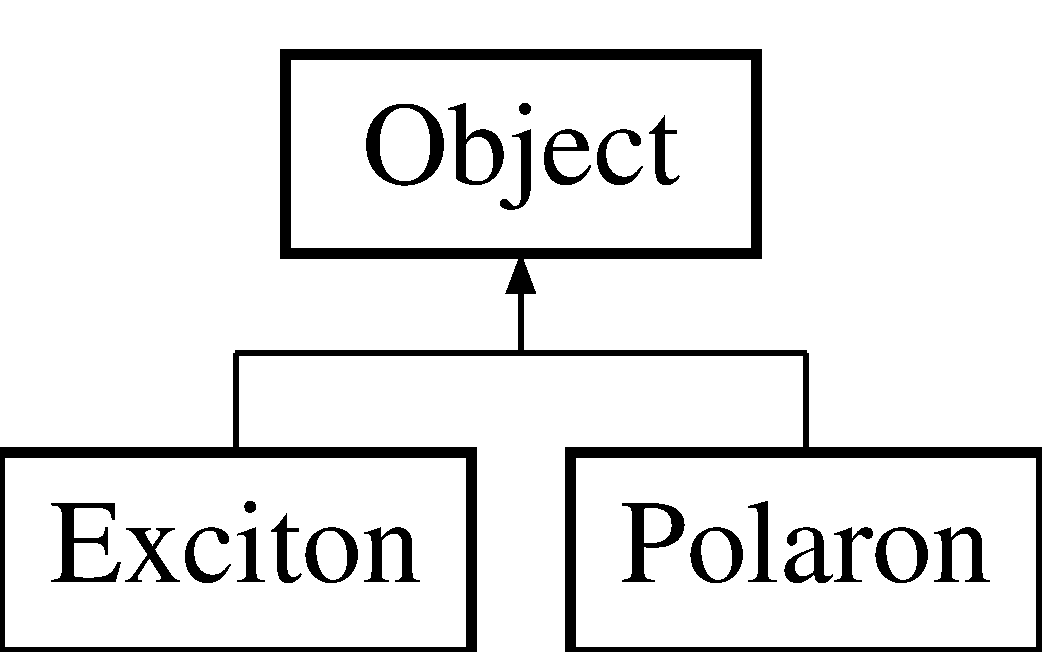
\includegraphics[height=2.000000cm]{class_object}
\end{center}
\end{figure}
\subsection*{Public Member Functions}
\begin{DoxyCompactItemize}
\item 
\mbox{\Hypertarget{class_object_ae8f5483f459e46687bd01e6f9977afd3}\label{class_object_ae8f5483f459e46687bd01e6f9977afd3}} 
virtual \hyperlink{class_object_ae8f5483f459e46687bd01e6f9977afd3}{$\sim$\+Object} ()
\begin{DoxyCompactList}\small\item\em Default virtual destructor needed by the base class. \end{DoxyCompactList}\item 
\mbox{\Hypertarget{class_object_a40860402e64d8008fb42329df7097cdb}\label{class_object_a40860402e64d8008fb42329df7097cdb}} 
\hyperlink{class_object_a40860402e64d8008fb42329df7097cdb}{Object} ()
\begin{DoxyCompactList}\small\item\em Default constructor that creates an empty \hyperlink{class_object}{Object} object. \end{DoxyCompactList}\item 
\hyperlink{class_object_aff050a622272cc7667251c7315f09fd7}{Object} (const double time, const int tag\+\_\+num, const \hyperlink{struct_coords}{Coords} \&start\+\_\+coords)
\begin{DoxyCompactList}\small\item\em Constructor that creates and initializes a usable \hyperlink{class_object}{Object} object. \end{DoxyCompactList}\item 
double \hyperlink{class_object_a02643ea0804dec3e43f60c788855c03b}{calculate\+Displacement} () const
\begin{DoxyCompactList}\small\item\em Calculates the displacement of the object from its starting coordinates in lattice units. \end{DoxyCompactList}\item 
\hyperlink{struct_coords}{Coords} \hyperlink{class_object_a08df08943dc634609fa69b356a37d73f}{get\+Coords} () const
\begin{DoxyCompactList}\small\item\em Gets the current coordinates of the \hyperlink{class_object}{Object}. \end{DoxyCompactList}\item 
double \hyperlink{class_object_a6f91c3f8b61cb9c9a8db662ac07d92e9}{get\+Creation\+Time} () const
\begin{DoxyCompactList}\small\item\em Gets the simulation creation time of the \hyperlink{class_object}{Object}. \end{DoxyCompactList}\item 
std\+::list$<$ \hyperlink{class_event}{Event} $\ast$ $>$\+::iterator \hyperlink{class_object_aa7c58e0319b7715c8d36f38ca7acf03e}{get\+Event\+It} () const
\begin{DoxyCompactList}\small\item\em Gets the event list iterator for the event that is associated with the object. \end{DoxyCompactList}\item 
virtual std\+::string \hyperlink{class_object_ade517616d51cd9ab581ec5afeb37b313}{get\+Name} () const
\begin{DoxyCompactList}\small\item\em Gets the name of the \hyperlink{class_object}{Object} class. \end{DoxyCompactList}\item 
int \hyperlink{class_object_aa9653577e8d0ac4b7b86d23d12f8b31b}{get\+Tag} () const
\begin{DoxyCompactList}\small\item\em Gets the tag id number of the \hyperlink{class_object}{Object}. \end{DoxyCompactList}\item 
void \hyperlink{class_object_a3d7c877f4aa179d9a56050c5faddc18d}{increment\+DX} (const int num)
\begin{DoxyCompactList}\small\item\em Increments the dx parameter, which is to be used when the \hyperlink{class_object}{Object} crosses an x-\/direction periodic boundary. \end{DoxyCompactList}\item 
void \hyperlink{class_object_a9df010818be72d15bad7985bf8a89ba0}{increment\+DY} (const int num)
\begin{DoxyCompactList}\small\item\em Increments the dy parameter, which is to be used when the \hyperlink{class_object}{Object} crosses a y-\/direction periodic boundary. \end{DoxyCompactList}\item 
void \hyperlink{class_object_a440b267c478f5d63db1954bdbd543408}{increment\+DZ} (const int num)
\begin{DoxyCompactList}\small\item\em Increments the dz parameter, which is to be used when the \hyperlink{class_object}{Object} crosses a z-\/direction periodic boundary. \end{DoxyCompactList}\item 
void \hyperlink{class_object_a34a164e4709e5daaba7a38c3d61ae617}{set\+Coords} (const \hyperlink{struct_coords}{Coords} \&input\+\_\+coords)
\begin{DoxyCompactList}\small\item\em Sets the coordinates of the \hyperlink{class_object}{Object}. \end{DoxyCompactList}\item 
void \hyperlink{class_object_ad5025bd84ae91d6426f458f32e582293}{set\+Event\+It} (const std\+::list$<$ \hyperlink{class_event}{Event} $\ast$$>$\+::iterator input\+\_\+it)
\begin{DoxyCompactList}\small\item\em Sets the iterator that points to a specific entry in the events list within the \hyperlink{class_simulation}{Simulation} class. \end{DoxyCompactList}\end{DoxyCompactItemize}


\subsection{Detailed Description}
This base class contains the basic properties of a K\+MC simulation object and the functions needed to interact with it. 

This base class is designed to work with the \hyperlink{class_simulation}{Simulation} class to construct a K\+MC simulation. This base class is intended to be extended to create classes that represent specific types of objects. \begin{DoxyCopyright}{Copyright}
M\+IT License. For more information, see the L\+I\+C\+E\+N\+SE file that accompanies this software package. 
\end{DoxyCopyright}
\begin{DoxyAuthor}{Author}
Michael C. Heiber 
\end{DoxyAuthor}
\begin{DoxyDate}{Date}
2017 
\end{DoxyDate}


\subsection{Constructor \& Destructor Documentation}
\mbox{\Hypertarget{class_object_aff050a622272cc7667251c7315f09fd7}\label{class_object_aff050a622272cc7667251c7315f09fd7}} 
\index{Object@{Object}!Object@{Object}}
\index{Object@{Object}!Object@{Object}}
\subsubsection{\texorpdfstring{Object()}{Object()}}
{\footnotesize\ttfamily Object\+::\+Object (\begin{DoxyParamCaption}\item[{const double}]{time,  }\item[{const int}]{tag\+\_\+num,  }\item[{const \hyperlink{struct_coords}{Coords} \&}]{start\+\_\+coords }\end{DoxyParamCaption})}



Constructor that creates and initializes a usable \hyperlink{class_object}{Object} object. 


\begin{DoxyParams}{Parameters}
{\em time} & is the current simulation time. \\
\hline
{\em tag\+\_\+num} & is the specified tag ID number that will be used to label the \hyperlink{class_object}{Object}. \\
\hline
{\em start\+\_\+coords} & is the \hyperlink{struct_coords}{Coords} struct that defines the starting coordinates of the \hyperlink{class_object}{Object}. \\
\hline
\end{DoxyParams}


\subsection{Member Function Documentation}
\mbox{\Hypertarget{class_object_a02643ea0804dec3e43f60c788855c03b}\label{class_object_a02643ea0804dec3e43f60c788855c03b}} 
\index{Object@{Object}!calculate\+Displacement@{calculate\+Displacement}}
\index{calculate\+Displacement@{calculate\+Displacement}!Object@{Object}}
\subsubsection{\texorpdfstring{calculate\+Displacement()}{calculateDisplacement()}}
{\footnotesize\ttfamily double Object\+::calculate\+Displacement (\begin{DoxyParamCaption}{ }\end{DoxyParamCaption}) const}



Calculates the displacement of the object from its starting coordinates in lattice units. 

The function accounts for when periodic boundaries are crossed to determine the real displacement distance. \mbox{\Hypertarget{class_object_a08df08943dc634609fa69b356a37d73f}\label{class_object_a08df08943dc634609fa69b356a37d73f}} 
\index{Object@{Object}!get\+Coords@{get\+Coords}}
\index{get\+Coords@{get\+Coords}!Object@{Object}}
\subsubsection{\texorpdfstring{get\+Coords()}{getCoords()}}
{\footnotesize\ttfamily \hyperlink{struct_coords}{Coords} Object\+::get\+Coords (\begin{DoxyParamCaption}{ }\end{DoxyParamCaption}) const}



Gets the current coordinates of the \hyperlink{class_object}{Object}. 

\begin{DoxyReturn}{Returns}
a \hyperlink{struct_coords}{Coords} struct that represents the coordinates of the object. 
\end{DoxyReturn}
\mbox{\Hypertarget{class_object_a6f91c3f8b61cb9c9a8db662ac07d92e9}\label{class_object_a6f91c3f8b61cb9c9a8db662ac07d92e9}} 
\index{Object@{Object}!get\+Creation\+Time@{get\+Creation\+Time}}
\index{get\+Creation\+Time@{get\+Creation\+Time}!Object@{Object}}
\subsubsection{\texorpdfstring{get\+Creation\+Time()}{getCreationTime()}}
{\footnotesize\ttfamily double Object\+::get\+Creation\+Time (\begin{DoxyParamCaption}{ }\end{DoxyParamCaption}) const}



Gets the simulation creation time of the \hyperlink{class_object}{Object}. 

\begin{DoxyReturn}{Returns}
The simulation time value at which the object was created in units of seconds. 
\end{DoxyReturn}
\mbox{\Hypertarget{class_object_aa7c58e0319b7715c8d36f38ca7acf03e}\label{class_object_aa7c58e0319b7715c8d36f38ca7acf03e}} 
\index{Object@{Object}!get\+Event\+It@{get\+Event\+It}}
\index{get\+Event\+It@{get\+Event\+It}!Object@{Object}}
\subsubsection{\texorpdfstring{get\+Event\+It()}{getEventIt()}}
{\footnotesize\ttfamily list$<$ \hyperlink{class_event}{Event} $\ast$ $>$\+::iterator Object\+::get\+Event\+It (\begin{DoxyParamCaption}{ }\end{DoxyParamCaption}) const}



Gets the event list iterator for the event that is associated with the object. 

The event list iterator points to an \hyperlink{class_event}{Event} pointer in the events list within the \hyperlink{class_simulation}{Simulation} class, and the \hyperlink{class_event}{Event} pointer points to a specific derived \hyperlink{class_event}{Event} class stored in the derived \hyperlink{class_simulation}{Simulation} class. \mbox{\Hypertarget{class_object_ade517616d51cd9ab581ec5afeb37b313}\label{class_object_ade517616d51cd9ab581ec5afeb37b313}} 
\index{Object@{Object}!get\+Name@{get\+Name}}
\index{get\+Name@{get\+Name}!Object@{Object}}
\subsubsection{\texorpdfstring{get\+Name()}{getName()}}
{\footnotesize\ttfamily string Object\+::get\+Name (\begin{DoxyParamCaption}{ }\end{DoxyParamCaption}) const\hspace{0.3cm}{\ttfamily [virtual]}}



Gets the name of the \hyperlink{class_object}{Object} class. 

\begin{DoxyReturn}{Returns}
\char`\"{}\+Object\char`\"{} when called on the base class. 
\end{DoxyReturn}


Reimplemented in \hyperlink{class_exciton_a4db43bd7ca4136e35f9a50b2a5854728}{Exciton}, and \hyperlink{class_polaron_ab30575f6248183c9dab4d257df2f91fc}{Polaron}.

\mbox{\Hypertarget{class_object_aa9653577e8d0ac4b7b86d23d12f8b31b}\label{class_object_aa9653577e8d0ac4b7b86d23d12f8b31b}} 
\index{Object@{Object}!get\+Tag@{get\+Tag}}
\index{get\+Tag@{get\+Tag}!Object@{Object}}
\subsubsection{\texorpdfstring{get\+Tag()}{getTag()}}
{\footnotesize\ttfamily int Object\+::get\+Tag (\begin{DoxyParamCaption}{ }\end{DoxyParamCaption}) const}



Gets the tag id number of the \hyperlink{class_object}{Object}. 

\begin{DoxyWarning}{Warning}
This tag id number may not be unique between objects that are of different derived object classes. 
\end{DoxyWarning}
\mbox{\Hypertarget{class_object_a3d7c877f4aa179d9a56050c5faddc18d}\label{class_object_a3d7c877f4aa179d9a56050c5faddc18d}} 
\index{Object@{Object}!increment\+DX@{increment\+DX}}
\index{increment\+DX@{increment\+DX}!Object@{Object}}
\subsubsection{\texorpdfstring{increment\+D\+X()}{incrementDX()}}
{\footnotesize\ttfamily void Object\+::increment\+DX (\begin{DoxyParamCaption}\item[{const int}]{num }\end{DoxyParamCaption})}



Increments the dx parameter, which is to be used when the \hyperlink{class_object}{Object} crosses an x-\/direction periodic boundary. 


\begin{DoxyParams}{Parameters}
{\em num} & is the input increment amount. \\
\hline
\end{DoxyParams}
\mbox{\Hypertarget{class_object_a9df010818be72d15bad7985bf8a89ba0}\label{class_object_a9df010818be72d15bad7985bf8a89ba0}} 
\index{Object@{Object}!increment\+DY@{increment\+DY}}
\index{increment\+DY@{increment\+DY}!Object@{Object}}
\subsubsection{\texorpdfstring{increment\+D\+Y()}{incrementDY()}}
{\footnotesize\ttfamily void Object\+::increment\+DY (\begin{DoxyParamCaption}\item[{const int}]{num }\end{DoxyParamCaption})}



Increments the dy parameter, which is to be used when the \hyperlink{class_object}{Object} crosses a y-\/direction periodic boundary. 


\begin{DoxyParams}{Parameters}
{\em num} & is the input increment amount. \\
\hline
\end{DoxyParams}
\mbox{\Hypertarget{class_object_a440b267c478f5d63db1954bdbd543408}\label{class_object_a440b267c478f5d63db1954bdbd543408}} 
\index{Object@{Object}!increment\+DZ@{increment\+DZ}}
\index{increment\+DZ@{increment\+DZ}!Object@{Object}}
\subsubsection{\texorpdfstring{increment\+D\+Z()}{incrementDZ()}}
{\footnotesize\ttfamily void Object\+::increment\+DZ (\begin{DoxyParamCaption}\item[{const int}]{num }\end{DoxyParamCaption})}



Increments the dz parameter, which is to be used when the \hyperlink{class_object}{Object} crosses a z-\/direction periodic boundary. 


\begin{DoxyParams}{Parameters}
{\em num} & is the input increment amount. \\
\hline
\end{DoxyParams}
\mbox{\Hypertarget{class_object_a34a164e4709e5daaba7a38c3d61ae617}\label{class_object_a34a164e4709e5daaba7a38c3d61ae617}} 
\index{Object@{Object}!set\+Coords@{set\+Coords}}
\index{set\+Coords@{set\+Coords}!Object@{Object}}
\subsubsection{\texorpdfstring{set\+Coords()}{setCoords()}}
{\footnotesize\ttfamily void Object\+::set\+Coords (\begin{DoxyParamCaption}\item[{const \hyperlink{struct_coords}{Coords} \&}]{input\+\_\+coords }\end{DoxyParamCaption})}



Sets the coordinates of the \hyperlink{class_object}{Object}. 


\begin{DoxyParams}{Parameters}
{\em input\+\_\+coords} & is the \hyperlink{struct_coords}{Coords} struct that designates the input coordinates. \\
\hline
\end{DoxyParams}
\mbox{\Hypertarget{class_object_ad5025bd84ae91d6426f458f32e582293}\label{class_object_ad5025bd84ae91d6426f458f32e582293}} 
\index{Object@{Object}!set\+Event\+It@{set\+Event\+It}}
\index{set\+Event\+It@{set\+Event\+It}!Object@{Object}}
\subsubsection{\texorpdfstring{set\+Event\+It()}{setEventIt()}}
{\footnotesize\ttfamily void Object\+::set\+Event\+It (\begin{DoxyParamCaption}\item[{const std\+::list$<$ \hyperlink{class_event}{Event} $\ast$$>$\+::iterator}]{input\+\_\+it }\end{DoxyParamCaption})}



Sets the iterator that points to a specific entry in the events list within the \hyperlink{class_simulation}{Simulation} class. 


\begin{DoxyParams}{Parameters}
{\em input\+\_\+it} & is the input event list iterator. \\
\hline
\end{DoxyParams}


The documentation for this class was generated from the following files\+:\begin{DoxyCompactItemize}
\item 
K\+M\+C\+\_\+\+Lattice/Object.\+h\item 
K\+M\+C\+\_\+\+Lattice/Object.\+cpp\end{DoxyCompactItemize}

\hypertarget{class_o_s_c___sim}{}\section{O\+S\+C\+\_\+\+Sim Class Reference}
\label{class_o_s_c___sim}\index{O\+S\+C\+\_\+\+Sim@{O\+S\+C\+\_\+\+Sim}}
Inheritance diagram for O\+S\+C\+\_\+\+Sim\+:\begin{figure}[H]
\begin{center}
\leavevmode
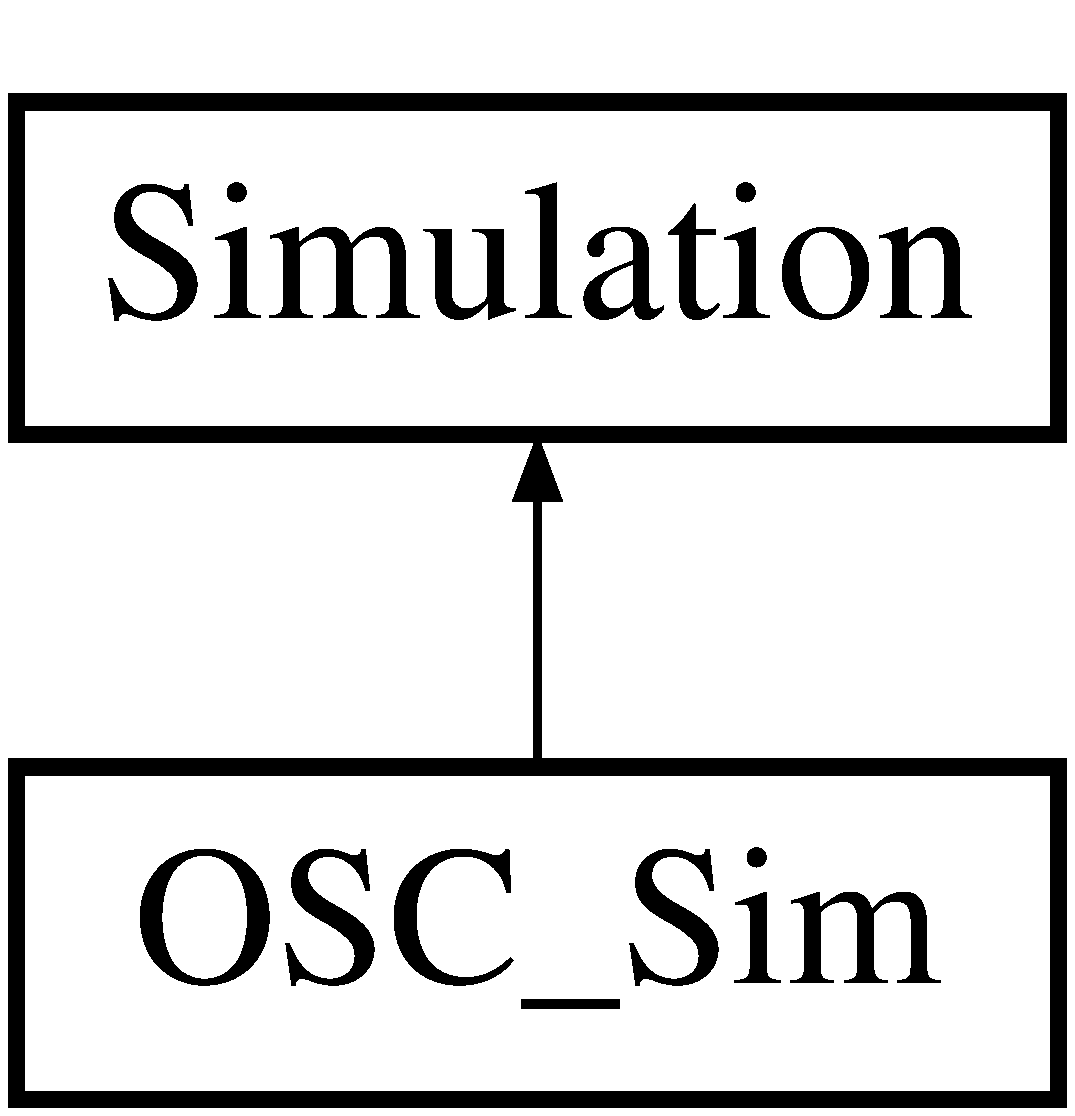
\includegraphics[height=2.000000cm]{class_o_s_c___sim}
\end{center}
\end{figure}
\subsection*{Public Member Functions}
\begin{DoxyCompactItemize}
\item 
\mbox{\Hypertarget{class_o_s_c___sim_a7c6cce40287a60c271509c1f3d8eef9a}\label{class_o_s_c___sim_a7c6cce40287a60c271509c1f3d8eef9a}} 
bool {\bfseries init} (const \hyperlink{struct_parameters___o_p_v}{Parameters\+\_\+\+O\+PV} \&params, const int id)
\item 
\mbox{\Hypertarget{class_o_s_c___sim_a62aa25ac6740cea4efab1dcc7f88c5d5}\label{class_o_s_c___sim_a62aa25ac6740cea4efab1dcc7f88c5d5}} 
double {\bfseries calculate\+Diffusion\+Length\+\_\+avg} () const
\item 
\mbox{\Hypertarget{class_o_s_c___sim_a858300b2a76f1a1b24747d11869a1f4a}\label{class_o_s_c___sim_a858300b2a76f1a1b24747d11869a1f4a}} 
double {\bfseries calculate\+Diffusion\+Length\+\_\+stdev} () const
\item 
\mbox{\Hypertarget{class_o_s_c___sim_afdd01fa07d004b0c37ce86ee171a60b8}\label{class_o_s_c___sim_afdd01fa07d004b0c37ce86ee171a60b8}} 
std\+::vector$<$ std\+::pair$<$ double, double $>$ $>$ {\bfseries calculate\+D\+O\+S\+Correlation} (const double cutoff\+\_\+radius)
\item 
\mbox{\Hypertarget{class_o_s_c___sim_a176ab132e314dfd509e8feb89687f163}\label{class_o_s_c___sim_a176ab132e314dfd509e8feb89687f163}} 
std\+::vector$<$ double $>$ {\bfseries calculate\+Transit\+Time\+Dist} (const std\+::vector$<$ double $>$ \&data, const int counts) const
\item 
\mbox{\Hypertarget{class_o_s_c___sim_a99e37cc427f843a92d58c6fa9b13fffe}\label{class_o_s_c___sim_a99e37cc427f843a92d58c6fa9b13fffe}} 
double {\bfseries calculate\+Transit\+Time\+\_\+avg} () const
\item 
\mbox{\Hypertarget{class_o_s_c___sim_a7e7da89362449d58373a31c255a27d8f}\label{class_o_s_c___sim_a7e7da89362449d58373a31c255a27d8f}} 
double {\bfseries calculate\+Transit\+Time\+\_\+stdev} () const
\item 
\mbox{\Hypertarget{class_o_s_c___sim_a8cbaab921f75c2b1ccc85b42ed698c58}\label{class_o_s_c___sim_a8cbaab921f75c2b1ccc85b42ed698c58}} 
std\+::vector$<$ double $>$ {\bfseries calculate\+Mobilities} (const std\+::vector$<$ double $>$ \&transit\+\_\+times) const
\item 
\mbox{\Hypertarget{class_o_s_c___sim_aef139f85af869c000b362b2a17e46cff}\label{class_o_s_c___sim_aef139f85af869c000b362b2a17e46cff}} 
double {\bfseries calculate\+Mobility\+\_\+avg} () const
\item 
\mbox{\Hypertarget{class_o_s_c___sim_a7cbca947933286e632d3d76dfed403bf}\label{class_o_s_c___sim_a7cbca947933286e632d3d76dfed403bf}} 
double {\bfseries calculate\+Mobility\+\_\+stdev} () const
\item 
bool \hyperlink{class_o_s_c___sim_ab3e4258c850b48ec02e4d3a88b583115}{check\+Finished} () const
\begin{DoxyCompactList}\small\item\em Checks whether or not the simulation has finished. \end{DoxyCompactList}\item 
\mbox{\Hypertarget{class_o_s_c___sim_a92f8e2ae6bcd3e0755feb2419849c8e9}\label{class_o_s_c___sim_a92f8e2ae6bcd3e0755feb2419849c8e9}} 
bool {\bfseries check\+Parameters} (const \hyperlink{struct_parameters___o_p_v}{Parameters\+\_\+\+O\+PV} \&params) const
\item 
bool \hyperlink{class_o_s_c___sim_a41bdb6368c71e1a3cb0efdc2a55d7869}{execute\+Next\+Event} ()
\begin{DoxyCompactList}\small\item\em Executes the next event in the simulation. \end{DoxyCompactList}\item 
\mbox{\Hypertarget{class_o_s_c___sim_a97f04719b91c90ac64dd8186476aa5f5}\label{class_o_s_c___sim_a97f04719b91c90ac64dd8186476aa5f5}} 
std\+::vector$<$ double $>$ {\bfseries get\+Diffusion\+Data} () const
\item 
\mbox{\Hypertarget{class_o_s_c___sim_a804f8facf0f5ee86d0234662a0719571}\label{class_o_s_c___sim_a804f8facf0f5ee86d0234662a0719571}} 
std\+::vector$<$ std\+::pair$<$ double, double $>$ $>$ {\bfseries get\+D\+O\+S\+Correlation\+Data} () const
\item 
\mbox{\Hypertarget{class_o_s_c___sim_a16f5ce34d8cb54220ce09998e6dff46f}\label{class_o_s_c___sim_a16f5ce34d8cb54220ce09998e6dff46f}} 
std\+::vector$<$ int $>$ {\bfseries get\+Dynamics\+Transient\+Excitons} () const
\item 
\mbox{\Hypertarget{class_o_s_c___sim_a53be32d48cc8319af6143fe858b3840f}\label{class_o_s_c___sim_a53be32d48cc8319af6143fe858b3840f}} 
std\+::vector$<$ int $>$ {\bfseries get\+Dynamics\+Transient\+Electrons} () const
\item 
\mbox{\Hypertarget{class_o_s_c___sim_ad6bffe074bd5e2c5b2f08561fa8bf117}\label{class_o_s_c___sim_ad6bffe074bd5e2c5b2f08561fa8bf117}} 
std\+::vector$<$ int $>$ {\bfseries get\+Dynamics\+Transient\+Holes} () const
\item 
\mbox{\Hypertarget{class_o_s_c___sim_acde6068549f59f813d2faed73f6fedc9}\label{class_o_s_c___sim_acde6068549f59f813d2faed73f6fedc9}} 
std\+::vector$<$ double $>$ {\bfseries get\+Dynamics\+Transient\+Times} () const
\item 
\mbox{\Hypertarget{class_o_s_c___sim_aae233390486c4db28a72936dd7d398f1}\label{class_o_s_c___sim_aae233390486c4db28a72936dd7d398f1}} 
std\+::vector$<$ double $>$ {\bfseries get\+Site\+Energies} (const short site\+\_\+type) const
\item 
\mbox{\Hypertarget{class_o_s_c___sim_a6ce1e72c2a7d1161f844ebd46231c961}\label{class_o_s_c___sim_a6ce1e72c2a7d1161f844ebd46231c961}} 
std\+::vector$<$ std\+::string $>$ {\bfseries get\+Charge\+Extraction\+Map} (const bool charge) const
\item 
\mbox{\Hypertarget{class_o_s_c___sim_aa3e0342b2a8c7dc5a62211dd6161027f}\label{class_o_s_c___sim_aa3e0342b2a8c7dc5a62211dd6161027f}} 
std\+::vector$<$ int $>$ {\bfseries get\+To\+F\+Transient\+Counts} () const
\item 
\mbox{\Hypertarget{class_o_s_c___sim_a03028810d8edc276ed7ab0a8228feaaa}\label{class_o_s_c___sim_a03028810d8edc276ed7ab0a8228feaaa}} 
std\+::vector$<$ double $>$ {\bfseries get\+To\+F\+Transient\+Energies} () const
\item 
\mbox{\Hypertarget{class_o_s_c___sim_a01a190017bc7a7e04c6af824fa47dbce}\label{class_o_s_c___sim_a01a190017bc7a7e04c6af824fa47dbce}} 
std\+::vector$<$ double $>$ {\bfseries get\+To\+F\+Transient\+Times} () const
\item 
\mbox{\Hypertarget{class_o_s_c___sim_a15a47ed6657c8301eac0c938f8887324}\label{class_o_s_c___sim_a15a47ed6657c8301eac0c938f8887324}} 
std\+::vector$<$ double $>$ {\bfseries get\+To\+F\+Transient\+Velocities} () const
\item 
\mbox{\Hypertarget{class_o_s_c___sim_ac5a6b2ae37d49b9114fe032f533e41c6}\label{class_o_s_c___sim_ac5a6b2ae37d49b9114fe032f533e41c6}} 
std\+::vector$<$ double $>$ {\bfseries get\+Transit\+Time\+Data} () const
\item 
\mbox{\Hypertarget{class_o_s_c___sim_ad38ee5ecfdd65fe4d162763842a2a4b6}\label{class_o_s_c___sim_ad38ee5ecfdd65fe4d162763842a2a4b6}} 
int {\bfseries get\+N\+\_\+excitons\+\_\+created} () const
\item 
\mbox{\Hypertarget{class_o_s_c___sim_a3159c7445f114390c7fb52fa73d559ef}\label{class_o_s_c___sim_a3159c7445f114390c7fb52fa73d559ef}} 
int {\bfseries get\+N\+\_\+excitons\+\_\+created} (const short site\+\_\+type) const
\item 
\mbox{\Hypertarget{class_o_s_c___sim_ad4e1d01074aa99ab83a86caf102ed1f0}\label{class_o_s_c___sim_ad4e1d01074aa99ab83a86caf102ed1f0}} 
int {\bfseries get\+N\+\_\+excitons\+\_\+dissociated} () const
\item 
\mbox{\Hypertarget{class_o_s_c___sim_af4b5988d7867fd1d6d297768c758d984}\label{class_o_s_c___sim_af4b5988d7867fd1d6d297768c758d984}} 
int {\bfseries get\+N\+\_\+excitons\+\_\+recombined} () const
\item 
\mbox{\Hypertarget{class_o_s_c___sim_aadb3c72821bac6153f0f848ce1a87c2b}\label{class_o_s_c___sim_aadb3c72821bac6153f0f848ce1a87c2b}} 
int {\bfseries get\+N\+\_\+electrons\+\_\+created} () const
\item 
\mbox{\Hypertarget{class_o_s_c___sim_abb8a9aefba0cb189fbaeba0f9bdff180}\label{class_o_s_c___sim_abb8a9aefba0cb189fbaeba0f9bdff180}} 
int {\bfseries get\+N\+\_\+electrons\+\_\+collected} () const
\item 
\mbox{\Hypertarget{class_o_s_c___sim_a15b6b1af56c4285252c6102b3672481c}\label{class_o_s_c___sim_a15b6b1af56c4285252c6102b3672481c}} 
int {\bfseries get\+N\+\_\+electrons\+\_\+recombined} () const
\item 
\mbox{\Hypertarget{class_o_s_c___sim_ae6bc3f06e216d922075039c6e3f900c9}\label{class_o_s_c___sim_ae6bc3f06e216d922075039c6e3f900c9}} 
int {\bfseries get\+N\+\_\+holes\+\_\+created} () const
\item 
\mbox{\Hypertarget{class_o_s_c___sim_a6809c1bc0b9fd7852621a86eb49457e0}\label{class_o_s_c___sim_a6809c1bc0b9fd7852621a86eb49457e0}} 
int {\bfseries get\+N\+\_\+holes\+\_\+collected} () const
\item 
\mbox{\Hypertarget{class_o_s_c___sim_aa6a8cfccbe629cba8ed137e3c205affe}\label{class_o_s_c___sim_aa6a8cfccbe629cba8ed137e3c205affe}} 
int {\bfseries get\+N\+\_\+holes\+\_\+recombined} () const
\item 
\mbox{\Hypertarget{class_o_s_c___sim_a152520ae80b5f879578c01c25b9b4a7f}\label{class_o_s_c___sim_a152520ae80b5f879578c01c25b9b4a7f}} 
int {\bfseries get\+N\+\_\+geminate\+\_\+recombinations} () const
\item 
\mbox{\Hypertarget{class_o_s_c___sim_afa814164790477d643fe04fca021483d}\label{class_o_s_c___sim_afa814164790477d643fe04fca021483d}} 
int {\bfseries get\+N\+\_\+bimolecular\+\_\+recombinations} () const
\item 
\mbox{\Hypertarget{class_o_s_c___sim_a0b14455856a684c59ba7d496782b0941}\label{class_o_s_c___sim_a0b14455856a684c59ba7d496782b0941}} 
int {\bfseries get\+N\+\_\+transient\+\_\+cycles} () const
\item 
\mbox{\Hypertarget{class_o_s_c___sim_a78aa9badec9d28169b7b71b29e90c265}\label{class_o_s_c___sim_a78aa9badec9d28169b7b71b29e90c265}} 
void {\bfseries output\+Status} ()
\item 
\mbox{\Hypertarget{class_o_s_c___sim_a75f8094106ced73efaec99cc302f2aa9}\label{class_o_s_c___sim_a75f8094106ced73efaec99cc302f2aa9}} 
void {\bfseries reassign\+Site\+Energies} ()
\end{DoxyCompactItemize}
\subsection*{Additional Inherited Members}


\subsection{Member Function Documentation}
\mbox{\Hypertarget{class_o_s_c___sim_ab3e4258c850b48ec02e4d3a88b583115}\label{class_o_s_c___sim_ab3e4258c850b48ec02e4d3a88b583115}} 
\index{O\+S\+C\+\_\+\+Sim@{O\+S\+C\+\_\+\+Sim}!check\+Finished@{check\+Finished}}
\index{check\+Finished@{check\+Finished}!O\+S\+C\+\_\+\+Sim@{O\+S\+C\+\_\+\+Sim}}
\subsubsection{\texorpdfstring{check\+Finished()}{checkFinished()}}
{\footnotesize\ttfamily bool O\+S\+C\+\_\+\+Sim\+::check\+Finished (\begin{DoxyParamCaption}{ }\end{DoxyParamCaption}) const\hspace{0.3cm}{\ttfamily [virtual]}}



Checks whether or not the simulation has finished. 

This is a pure virtual function in the base class that must be defined by any derived class. \begin{DoxyReturn}{Returns}
true if the simulation is finished. 

false if the simulation is not finished. 
\end{DoxyReturn}


Implements \hyperlink{class_simulation_af69bb46977a3a0084214a194c888e16c}{Simulation}.

\mbox{\Hypertarget{class_o_s_c___sim_a41bdb6368c71e1a3cb0efdc2a55d7869}\label{class_o_s_c___sim_a41bdb6368c71e1a3cb0efdc2a55d7869}} 
\index{O\+S\+C\+\_\+\+Sim@{O\+S\+C\+\_\+\+Sim}!execute\+Next\+Event@{execute\+Next\+Event}}
\index{execute\+Next\+Event@{execute\+Next\+Event}!O\+S\+C\+\_\+\+Sim@{O\+S\+C\+\_\+\+Sim}}
\subsubsection{\texorpdfstring{execute\+Next\+Event()}{executeNextEvent()}}
{\footnotesize\ttfamily bool O\+S\+C\+\_\+\+Sim\+::execute\+Next\+Event (\begin{DoxyParamCaption}{ }\end{DoxyParamCaption})\hspace{0.3cm}{\ttfamily [virtual]}}



Executes the next event in the simulation. 

This is a pure virtual function in the base class that must be defined by any derived class. \begin{DoxyReturn}{Returns}
true if the next event is succesfully executed. 

false if execution of the next event is unsuccessful. 
\end{DoxyReturn}


Implements \hyperlink{class_simulation_a48e9e82f9dac1acec5d063a9f6f6115e}{Simulation}.



The documentation for this class was generated from the following files\+:\begin{DoxyCompactItemize}
\item 
O\+S\+C\+\_\+\+Sim.\+h\item 
O\+S\+C\+\_\+\+Sim.\+cpp\end{DoxyCompactItemize}

\hypertarget{struct_parameters___lattice}{}\section{Parameters\+\_\+\+Lattice Struct Reference}
\label{struct_parameters___lattice}\index{Parameters\+\_\+\+Lattice@{Parameters\+\_\+\+Lattice}}


This struct contains all of the main input parameters needed by the \hyperlink{class_lattice}{Lattice} class.  




{\ttfamily \#include $<$Lattice.\+h$>$}

\subsection*{Public Attributes}
\begin{DoxyCompactItemize}
\item 
\mbox{\Hypertarget{struct_parameters___lattice_a922f7e39f7debc0bd06ec1f0f1ca8257}\label{struct_parameters___lattice_a922f7e39f7debc0bd06ec1f0f1ca8257}} 
bool \hyperlink{struct_parameters___lattice_a922f7e39f7debc0bd06ec1f0f1ca8257}{Enable\+\_\+periodic\+\_\+x}
\begin{DoxyCompactList}\small\item\em Determines whether the x-\/direction periodic boundaries will be enabled. \end{DoxyCompactList}\item 
\mbox{\Hypertarget{struct_parameters___lattice_a9ee9c54330f7cd0bc32fd80e27ee87ff}\label{struct_parameters___lattice_a9ee9c54330f7cd0bc32fd80e27ee87ff}} 
bool \hyperlink{struct_parameters___lattice_a9ee9c54330f7cd0bc32fd80e27ee87ff}{Enable\+\_\+periodic\+\_\+y}
\begin{DoxyCompactList}\small\item\em Determines whether the y-\/direction periodic boundaries will be enabled. \end{DoxyCompactList}\item 
\mbox{\Hypertarget{struct_parameters___lattice_aff375c434a37560067d9cc677cff8052}\label{struct_parameters___lattice_aff375c434a37560067d9cc677cff8052}} 
bool \hyperlink{struct_parameters___lattice_aff375c434a37560067d9cc677cff8052}{Enable\+\_\+periodic\+\_\+z}
\begin{DoxyCompactList}\small\item\em Determines whether the z-\/direction periodic boundaries will be enabled. \end{DoxyCompactList}\item 
\mbox{\Hypertarget{struct_parameters___lattice_a99c7d553111bb660032bb7ca6f592da6}\label{struct_parameters___lattice_a99c7d553111bb660032bb7ca6f592da6}} 
int \hyperlink{struct_parameters___lattice_a99c7d553111bb660032bb7ca6f592da6}{Length}
\begin{DoxyCompactList}\small\item\em Defines the desired x-\/direction size of the lattice. \end{DoxyCompactList}\item 
\mbox{\Hypertarget{struct_parameters___lattice_a40f8633b47d204f471d041a0d8216e5b}\label{struct_parameters___lattice_a40f8633b47d204f471d041a0d8216e5b}} 
int \hyperlink{struct_parameters___lattice_a40f8633b47d204f471d041a0d8216e5b}{Width}
\begin{DoxyCompactList}\small\item\em Defines the desired y-\/direction size of the lattice. \end{DoxyCompactList}\item 
\mbox{\Hypertarget{struct_parameters___lattice_a1b59e1a307ad945fb86f44b68354f605}\label{struct_parameters___lattice_a1b59e1a307ad945fb86f44b68354f605}} 
int \hyperlink{struct_parameters___lattice_a1b59e1a307ad945fb86f44b68354f605}{Height}
\begin{DoxyCompactList}\small\item\em Defines the desired z-\/direction size of the lattice. \end{DoxyCompactList}\item 
\mbox{\Hypertarget{struct_parameters___lattice_a5f9628b968ba4206a7650c774827b1f0}\label{struct_parameters___lattice_a5f9628b968ba4206a7650c774827b1f0}} 
double \hyperlink{struct_parameters___lattice_a5f9628b968ba4206a7650c774827b1f0}{Unit\+\_\+size}
\begin{DoxyCompactList}\small\item\em Defines the desired lattice unit size, which is used to convert lattice units into real space units. \end{DoxyCompactList}\end{DoxyCompactItemize}


\subsection{Detailed Description}
This struct contains all of the main input parameters needed by the \hyperlink{class_lattice}{Lattice} class. 

\begin{DoxyCopyright}{Copyright}
M\+IT License. For more information, see the L\+I\+C\+E\+N\+SE file that accompanies this software package. 
\end{DoxyCopyright}
\begin{DoxyAuthor}{Author}
Michael C. Heiber 
\end{DoxyAuthor}
\begin{DoxyDate}{Date}
2017 
\end{DoxyDate}


The documentation for this struct was generated from the following file\+:\begin{DoxyCompactItemize}
\item 
K\+M\+C\+\_\+\+Lattice/Lattice.\+h\end{DoxyCompactItemize}

\hypertarget{struct_parameters__main}{}\section{Parameters\+\_\+main Struct Reference}
\label{struct_parameters__main}\index{Parameters\+\_\+main@{Parameters\+\_\+main}}
\subsection*{Public Attributes}
\begin{DoxyCompactItemize}
\item 
\mbox{\Hypertarget{struct_parameters__main_a619e840588f49eeba1c9d8757798c30e}\label{struct_parameters__main_a619e840588f49eeba1c9d8757798c30e}} 
bool {\bfseries Enable\+\_\+mpi}
\item 
\mbox{\Hypertarget{struct_parameters__main_a433c8fa80ee6c02fe5613d4eb2075546}\label{struct_parameters__main_a433c8fa80ee6c02fe5613d4eb2075546}} 
bool {\bfseries Enable\+\_\+import\+\_\+morphology\+\_\+single}
\item 
\mbox{\Hypertarget{struct_parameters__main_afa70eb9e8a4c918f678a26fa202650b1}\label{struct_parameters__main_afa70eb9e8a4c918f678a26fa202650b1}} 
string {\bfseries Morphology\+\_\+filename}
\item 
\mbox{\Hypertarget{struct_parameters__main_a8aa74759fabf23d020278b8b98a2d155}\label{struct_parameters__main_a8aa74759fabf23d020278b8b98a2d155}} 
bool {\bfseries Enable\+\_\+import\+\_\+morphology\+\_\+set}
\item 
\mbox{\Hypertarget{struct_parameters__main_afecfab3c5afbb2bc04ef3d5e8064c4a5}\label{struct_parameters__main_afecfab3c5afbb2bc04ef3d5e8064c4a5}} 
string {\bfseries Morphology\+\_\+set\+\_\+format}
\item 
\mbox{\Hypertarget{struct_parameters__main_a14e42c0e58188c19f860de2046cf796b}\label{struct_parameters__main_a14e42c0e58188c19f860de2046cf796b}} 
int {\bfseries N\+\_\+test\+\_\+morphologies}
\item 
\mbox{\Hypertarget{struct_parameters__main_a60ee2e45a155f2bef0681753e877bc5f}\label{struct_parameters__main_a60ee2e45a155f2bef0681753e877bc5f}} 
int {\bfseries N\+\_\+morphology\+\_\+set\+\_\+size}
\end{DoxyCompactItemize}


The documentation for this struct was generated from the following file\+:\begin{DoxyCompactItemize}
\item 
main.\+cpp\end{DoxyCompactItemize}

\hypertarget{struct_parameters___o_p_v}{}\section{Parameters\+\_\+\+O\+PV Struct Reference}
\label{struct_parameters___o_p_v}\index{Parameters\+\_\+\+O\+PV@{Parameters\+\_\+\+O\+PV}}
Inheritance diagram for Parameters\+\_\+\+O\+PV\+:\begin{figure}[H]
\begin{center}
\leavevmode
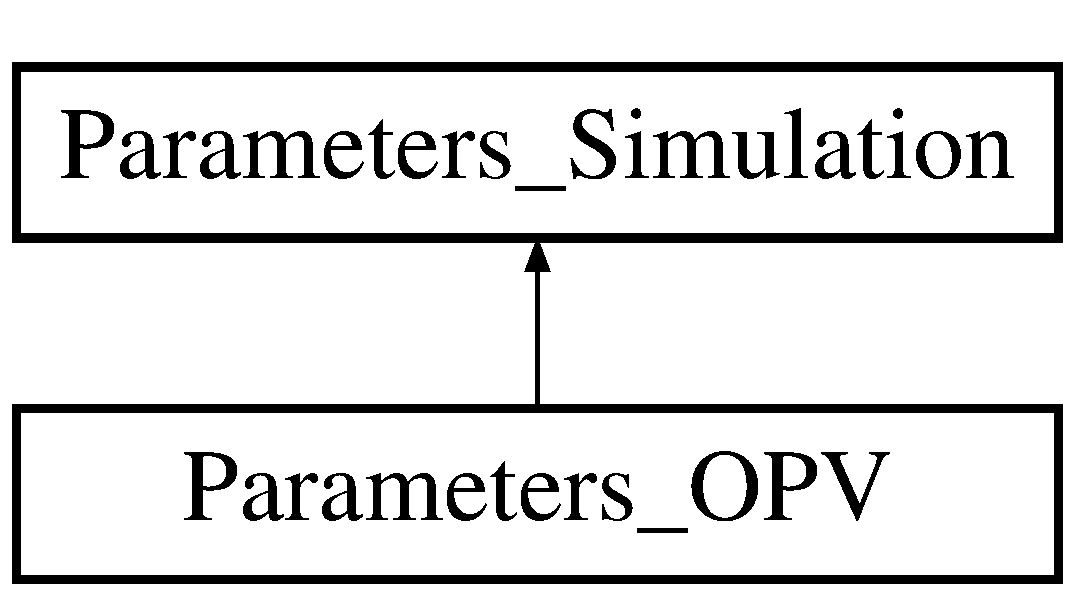
\includegraphics[height=2.000000cm]{struct_parameters___o_p_v}
\end{center}
\end{figure}
\subsection*{Public Attributes}
\begin{DoxyCompactItemize}
\item 
\mbox{\Hypertarget{struct_parameters___o_p_v_ac88bf3fcfbd5dbd502a05709e47d6540}\label{struct_parameters___o_p_v_ac88bf3fcfbd5dbd502a05709e47d6540}} 
double {\bfseries Bias}
\item 
\mbox{\Hypertarget{struct_parameters___o_p_v_ab935c4ae52bebea687d925e997fc8218}\label{struct_parameters___o_p_v_ab935c4ae52bebea687d925e997fc8218}} 
bool {\bfseries Enable\+\_\+neat}
\item 
\mbox{\Hypertarget{struct_parameters___o_p_v_a79f3ca42bb1073fac803ff8e74faabc0}\label{struct_parameters___o_p_v_a79f3ca42bb1073fac803ff8e74faabc0}} 
bool {\bfseries Enable\+\_\+bilayer}
\item 
\mbox{\Hypertarget{struct_parameters___o_p_v_a4c49f81e20e235e52f943003f0c14fa3}\label{struct_parameters___o_p_v_a4c49f81e20e235e52f943003f0c14fa3}} 
int {\bfseries Thickness\+\_\+donor}
\item 
\mbox{\Hypertarget{struct_parameters___o_p_v_afa28203f6b02b27ac415491bf1cb4f8a}\label{struct_parameters___o_p_v_afa28203f6b02b27ac415491bf1cb4f8a}} 
int {\bfseries Thickness\+\_\+acceptor}
\item 
\mbox{\Hypertarget{struct_parameters___o_p_v_a7d9cc030e67893f064dfb45b674f1d0e}\label{struct_parameters___o_p_v_a7d9cc030e67893f064dfb45b674f1d0e}} 
bool {\bfseries Enable\+\_\+random\+\_\+blend}
\item 
\mbox{\Hypertarget{struct_parameters___o_p_v_a21c46734660f2b2a55dbac798f6ea74b}\label{struct_parameters___o_p_v_a21c46734660f2b2a55dbac798f6ea74b}} 
double {\bfseries Acceptor\+\_\+conc}
\item 
\mbox{\Hypertarget{struct_parameters___o_p_v_aec3dc43adde4450252b30c2c705544cd}\label{struct_parameters___o_p_v_aec3dc43adde4450252b30c2c705544cd}} 
bool {\bfseries Enable\+\_\+import\+\_\+morphology}
\item 
\mbox{\Hypertarget{struct_parameters___o_p_v_a388e0f507abb6742efa33b1ca765ee13}\label{struct_parameters___o_p_v_a388e0f507abb6742efa33b1ca765ee13}} 
std\+::ifstream $\ast$ {\bfseries Morphology\+\_\+file}
\item 
\mbox{\Hypertarget{struct_parameters___o_p_v_a502f1711127656c15e78c7f1db168e0f}\label{struct_parameters___o_p_v_a502f1711127656c15e78c7f1db168e0f}} 
int {\bfseries N\+\_\+tests}
\item 
\mbox{\Hypertarget{struct_parameters___o_p_v_a12fc2fc3f18679ec9c9705085f89365a}\label{struct_parameters___o_p_v_a12fc2fc3f18679ec9c9705085f89365a}} 
bool {\bfseries Enable\+\_\+exciton\+\_\+diffusion\+\_\+test}
\item 
\mbox{\Hypertarget{struct_parameters___o_p_v_a323fbbb8b40716209cedf5b7c5c3a3e5}\label{struct_parameters___o_p_v_a323fbbb8b40716209cedf5b7c5c3a3e5}} 
bool {\bfseries Enable\+\_\+\+To\+F\+\_\+test}
\item 
\mbox{\Hypertarget{struct_parameters___o_p_v_a0a65769f9018d42e76e57244b20c4165}\label{struct_parameters___o_p_v_a0a65769f9018d42e76e57244b20c4165}} 
bool {\bfseries To\+F\+\_\+polaron\+\_\+type}
\item 
\mbox{\Hypertarget{struct_parameters___o_p_v_aa8d1f06c2e6e94b0b6bbf419d7b838aa}\label{struct_parameters___o_p_v_aa8d1f06c2e6e94b0b6bbf419d7b838aa}} 
int {\bfseries To\+F\+\_\+initial\+\_\+polarons}
\item 
\mbox{\Hypertarget{struct_parameters___o_p_v_af5e99b212ed3ece698fb032dd347af63}\label{struct_parameters___o_p_v_af5e99b212ed3ece698fb032dd347af63}} 
double {\bfseries To\+F\+\_\+transient\+\_\+start}
\item 
\mbox{\Hypertarget{struct_parameters___o_p_v_a6e17e68edee042fbcc30ccb06161dfb1}\label{struct_parameters___o_p_v_a6e17e68edee042fbcc30ccb06161dfb1}} 
double {\bfseries To\+F\+\_\+transient\+\_\+end}
\item 
\mbox{\Hypertarget{struct_parameters___o_p_v_ae89162ef61b8288b28e96ea1fe527da7}\label{struct_parameters___o_p_v_ae89162ef61b8288b28e96ea1fe527da7}} 
int {\bfseries To\+F\+\_\+pnts\+\_\+per\+\_\+decade}
\item 
\mbox{\Hypertarget{struct_parameters___o_p_v_ad3bc54415641c1f4c376fd3a4f30fdb4}\label{struct_parameters___o_p_v_ad3bc54415641c1f4c376fd3a4f30fdb4}} 
bool {\bfseries Enable\+\_\+\+I\+Q\+E\+\_\+test}
\item 
\mbox{\Hypertarget{struct_parameters___o_p_v_a03f47eeffc8a2984c03208ca2f84717d}\label{struct_parameters___o_p_v_a03f47eeffc8a2984c03208ca2f84717d}} 
double {\bfseries I\+Q\+E\+\_\+time\+\_\+cutoff}
\item 
\mbox{\Hypertarget{struct_parameters___o_p_v_ad634f90dda7176c038d14a81d07e272c}\label{struct_parameters___o_p_v_ad634f90dda7176c038d14a81d07e272c}} 
bool {\bfseries Enable\+\_\+dynamics\+\_\+test}
\item 
\mbox{\Hypertarget{struct_parameters___o_p_v_a14211060789d372a2c86e0bd859ca785}\label{struct_parameters___o_p_v_a14211060789d372a2c86e0bd859ca785}} 
bool {\bfseries Enable\+\_\+dynamics\+\_\+extraction}
\item 
\mbox{\Hypertarget{struct_parameters___o_p_v_a23e65440f36e8f28070c2392b01dd6b6}\label{struct_parameters___o_p_v_a23e65440f36e8f28070c2392b01dd6b6}} 
double {\bfseries Dynamics\+\_\+initial\+\_\+exciton\+\_\+conc}
\item 
\mbox{\Hypertarget{struct_parameters___o_p_v_a7cbc42f3e445821afb335f249b9dd680}\label{struct_parameters___o_p_v_a7cbc42f3e445821afb335f249b9dd680}} 
double {\bfseries Dynamics\+\_\+transient\+\_\+start}
\item 
\mbox{\Hypertarget{struct_parameters___o_p_v_a7964f93d211ecaa30c0b6b3e7397003d}\label{struct_parameters___o_p_v_a7964f93d211ecaa30c0b6b3e7397003d}} 
double {\bfseries Dynamics\+\_\+transient\+\_\+end}
\item 
\mbox{\Hypertarget{struct_parameters___o_p_v_a2506d3838ff71aac4853d7708f3ef74c}\label{struct_parameters___o_p_v_a2506d3838ff71aac4853d7708f3ef74c}} 
int {\bfseries Dynamics\+\_\+pnts\+\_\+per\+\_\+decade}
\item 
\mbox{\Hypertarget{struct_parameters___o_p_v_a4ceac22ea3ecbe7a6edab19e80d0783c}\label{struct_parameters___o_p_v_a4ceac22ea3ecbe7a6edab19e80d0783c}} 
double {\bfseries Exciton\+\_\+generation\+\_\+rate\+\_\+donor}
\item 
\mbox{\Hypertarget{struct_parameters___o_p_v_a33f99679368b91dcc39f305a658d793b}\label{struct_parameters___o_p_v_a33f99679368b91dcc39f305a658d793b}} 
double {\bfseries Exciton\+\_\+generation\+\_\+rate\+\_\+acceptor}
\item 
\mbox{\Hypertarget{struct_parameters___o_p_v_a4d772923d973c80fbd4b8fe18fec9f16}\label{struct_parameters___o_p_v_a4d772923d973c80fbd4b8fe18fec9f16}} 
double {\bfseries Singlet\+\_\+lifetime\+\_\+donor}
\item 
\mbox{\Hypertarget{struct_parameters___o_p_v_ab8ebcc4989f4b0fd5bfcd0ae59fb3ee6}\label{struct_parameters___o_p_v_ab8ebcc4989f4b0fd5bfcd0ae59fb3ee6}} 
double {\bfseries Singlet\+\_\+lifetime\+\_\+acceptor}
\item 
\mbox{\Hypertarget{struct_parameters___o_p_v_acb3f6fce76263baa95b6a20c7aeb5c4b}\label{struct_parameters___o_p_v_acb3f6fce76263baa95b6a20c7aeb5c4b}} 
double {\bfseries Triplet\+\_\+lifetime\+\_\+donor}
\item 
\mbox{\Hypertarget{struct_parameters___o_p_v_a4149a095d01c62295865a9064fccb637}\label{struct_parameters___o_p_v_a4149a095d01c62295865a9064fccb637}} 
double {\bfseries Triplet\+\_\+lifetime\+\_\+acceptor}
\item 
\mbox{\Hypertarget{struct_parameters___o_p_v_a292a5caeb412ff44bb829d06f22eebac}\label{struct_parameters___o_p_v_a292a5caeb412ff44bb829d06f22eebac}} 
double {\bfseries R\+\_\+singlet\+\_\+hopping\+\_\+donor}
\item 
\mbox{\Hypertarget{struct_parameters___o_p_v_addf89db7c365dc9c1c0ed5ac405c6e79}\label{struct_parameters___o_p_v_addf89db7c365dc9c1c0ed5ac405c6e79}} 
double {\bfseries R\+\_\+singlet\+\_\+hopping\+\_\+acceptor}
\item 
\mbox{\Hypertarget{struct_parameters___o_p_v_a8de2d7b5eac87daa32ece5ff4ec81917}\label{struct_parameters___o_p_v_a8de2d7b5eac87daa32ece5ff4ec81917}} 
double {\bfseries R\+\_\+triplet\+\_\+hopping\+\_\+donor}
\item 
\mbox{\Hypertarget{struct_parameters___o_p_v_a6e99571da45591efb83182cd95b72884}\label{struct_parameters___o_p_v_a6e99571da45591efb83182cd95b72884}} 
double {\bfseries R\+\_\+triplet\+\_\+hopping\+\_\+acceptor}
\item 
\mbox{\Hypertarget{struct_parameters___o_p_v_a5b7e58b86bfd90243849862f074ebf51}\label{struct_parameters___o_p_v_a5b7e58b86bfd90243849862f074ebf51}} 
double {\bfseries Triplet\+\_\+localization\+\_\+donor}
\item 
\mbox{\Hypertarget{struct_parameters___o_p_v_aac11d663f53039160f936a5c670151ed}\label{struct_parameters___o_p_v_aac11d663f53039160f936a5c670151ed}} 
double {\bfseries Triplet\+\_\+localization\+\_\+acceptor}
\item 
\mbox{\Hypertarget{struct_parameters___o_p_v_a2d31dc44f632afe90ee6218ac3509a5d}\label{struct_parameters___o_p_v_a2d31dc44f632afe90ee6218ac3509a5d}} 
bool {\bfseries Enable\+\_\+\+F\+R\+E\+T\+\_\+triplet\+\_\+annihilation}
\item 
\mbox{\Hypertarget{struct_parameters___o_p_v_a66580234d20375c017a3e9bad303062d}\label{struct_parameters___o_p_v_a66580234d20375c017a3e9bad303062d}} 
double {\bfseries R\+\_\+exciton\+\_\+exciton\+\_\+annihilation\+\_\+donor}
\item 
\mbox{\Hypertarget{struct_parameters___o_p_v_ad6159c82da14b1d66e1afd03d6e4bc00}\label{struct_parameters___o_p_v_ad6159c82da14b1d66e1afd03d6e4bc00}} 
double {\bfseries R\+\_\+exciton\+\_\+exciton\+\_\+annihilation\+\_\+acceptor}
\item 
\mbox{\Hypertarget{struct_parameters___o_p_v_ad4e469469b09cf493dc46a4ca1f60705}\label{struct_parameters___o_p_v_ad4e469469b09cf493dc46a4ca1f60705}} 
double {\bfseries R\+\_\+exciton\+\_\+polaron\+\_\+annihilation\+\_\+donor}
\item 
\mbox{\Hypertarget{struct_parameters___o_p_v_a8ce8b281ba79d02867f60e22142cf7c8}\label{struct_parameters___o_p_v_a8ce8b281ba79d02867f60e22142cf7c8}} 
double {\bfseries R\+\_\+exciton\+\_\+polaron\+\_\+annihilation\+\_\+acceptor}
\item 
\mbox{\Hypertarget{struct_parameters___o_p_v_a5fc92d26c86f41eb905da56629d483ef}\label{struct_parameters___o_p_v_a5fc92d26c86f41eb905da56629d483ef}} 
int {\bfseries F\+R\+E\+T\+\_\+cutoff}
\item 
\mbox{\Hypertarget{struct_parameters___o_p_v_ad23850399d27e4d8c6c3c803243e2712}\label{struct_parameters___o_p_v_ad23850399d27e4d8c6c3c803243e2712}} 
double {\bfseries E\+\_\+exciton\+\_\+binding\+\_\+donor}
\item 
\mbox{\Hypertarget{struct_parameters___o_p_v_a28998663eb890458a662eefc8f9ea0c9}\label{struct_parameters___o_p_v_a28998663eb890458a662eefc8f9ea0c9}} 
double {\bfseries E\+\_\+exciton\+\_\+binding\+\_\+acceptor}
\item 
\mbox{\Hypertarget{struct_parameters___o_p_v_ad021801a526f21ae43037f3e573d50e7}\label{struct_parameters___o_p_v_ad021801a526f21ae43037f3e573d50e7}} 
double {\bfseries R\+\_\+exciton\+\_\+dissociation\+\_\+donor}
\item 
\mbox{\Hypertarget{struct_parameters___o_p_v_aa52d0a4c9795976b4516e214104dd815}\label{struct_parameters___o_p_v_aa52d0a4c9795976b4516e214104dd815}} 
double {\bfseries R\+\_\+exciton\+\_\+dissociation\+\_\+acceptor}
\item 
\mbox{\Hypertarget{struct_parameters___o_p_v_ad4aaf3f56fe842bc998b3608c5b5b40b}\label{struct_parameters___o_p_v_ad4aaf3f56fe842bc998b3608c5b5b40b}} 
int {\bfseries Exciton\+\_\+dissociation\+\_\+cutoff}
\item 
\mbox{\Hypertarget{struct_parameters___o_p_v_a424ec76e06337bddcdd68550e448792f}\label{struct_parameters___o_p_v_a424ec76e06337bddcdd68550e448792f}} 
double {\bfseries R\+\_\+exciton\+\_\+isc\+\_\+donor}
\item 
\mbox{\Hypertarget{struct_parameters___o_p_v_a9ebd4980c4aa28e62f725e39f93fbc3b}\label{struct_parameters___o_p_v_a9ebd4980c4aa28e62f725e39f93fbc3b}} 
double {\bfseries R\+\_\+exciton\+\_\+isc\+\_\+acceptor}
\item 
\mbox{\Hypertarget{struct_parameters___o_p_v_ace6d9ab02c79ca3483988089e4c1b9a3}\label{struct_parameters___o_p_v_ace6d9ab02c79ca3483988089e4c1b9a3}} 
double {\bfseries R\+\_\+exciton\+\_\+risc\+\_\+donor}
\item 
\mbox{\Hypertarget{struct_parameters___o_p_v_ad6198eb075e56b1e69880d8323d7bf65}\label{struct_parameters___o_p_v_ad6198eb075e56b1e69880d8323d7bf65}} 
double {\bfseries R\+\_\+exciton\+\_\+risc\+\_\+acceptor}
\item 
\mbox{\Hypertarget{struct_parameters___o_p_v_a7f64bb8c308383c43240bd1e874239f8}\label{struct_parameters___o_p_v_a7f64bb8c308383c43240bd1e874239f8}} 
double {\bfseries E\+\_\+exciton\+\_\+\+S\+T\+\_\+donor}
\item 
\mbox{\Hypertarget{struct_parameters___o_p_v_a6731133a6dfb067c11a2073a2d6d748b}\label{struct_parameters___o_p_v_a6731133a6dfb067c11a2073a2d6d748b}} 
double {\bfseries E\+\_\+exciton\+\_\+\+S\+T\+\_\+acceptor}
\item 
\mbox{\Hypertarget{struct_parameters___o_p_v_ac43d697cf3102e9da550b62d7dc5c84c}\label{struct_parameters___o_p_v_ac43d697cf3102e9da550b62d7dc5c84c}} 
bool {\bfseries Enable\+\_\+phase\+\_\+restriction}
\item 
\mbox{\Hypertarget{struct_parameters___o_p_v_a8938dab01474122541123c605a25c56b}\label{struct_parameters___o_p_v_a8938dab01474122541123c605a25c56b}} 
double {\bfseries R\+\_\+polaron\+\_\+hopping\+\_\+donor}
\item 
\mbox{\Hypertarget{struct_parameters___o_p_v_ad84bb0a0fe56bb1f5157304f63d1503c}\label{struct_parameters___o_p_v_ad84bb0a0fe56bb1f5157304f63d1503c}} 
double {\bfseries R\+\_\+polaron\+\_\+hopping\+\_\+acceptor}
\item 
\mbox{\Hypertarget{struct_parameters___o_p_v_ac9f152101e3970f62d321eb02d211020}\label{struct_parameters___o_p_v_ac9f152101e3970f62d321eb02d211020}} 
double {\bfseries Polaron\+\_\+localization\+\_\+donor}
\item 
\mbox{\Hypertarget{struct_parameters___o_p_v_a794d79e512c2c161ab6242f5d372faef}\label{struct_parameters___o_p_v_a794d79e512c2c161ab6242f5d372faef}} 
double {\bfseries Polaron\+\_\+localization\+\_\+acceptor}
\item 
\mbox{\Hypertarget{struct_parameters___o_p_v_afeee51274483a1167c3dc3ca35c4de52}\label{struct_parameters___o_p_v_afeee51274483a1167c3dc3ca35c4de52}} 
bool {\bfseries Enable\+\_\+miller\+\_\+abrahams}
\item 
\mbox{\Hypertarget{struct_parameters___o_p_v_a3b4cef2f21e25714c83300b942f7daee}\label{struct_parameters___o_p_v_a3b4cef2f21e25714c83300b942f7daee}} 
bool {\bfseries Enable\+\_\+marcus}
\item 
\mbox{\Hypertarget{struct_parameters___o_p_v_a05158466d7973c098d8b6b5b4b43143c}\label{struct_parameters___o_p_v_a05158466d7973c098d8b6b5b4b43143c}} 
double {\bfseries Reorganization\+\_\+donor}
\item 
\mbox{\Hypertarget{struct_parameters___o_p_v_ab0a52db3d6358562603083f6839cf8ad}\label{struct_parameters___o_p_v_ab0a52db3d6358562603083f6839cf8ad}} 
double {\bfseries Reorganization\+\_\+acceptor}
\item 
\mbox{\Hypertarget{struct_parameters___o_p_v_a0e55f779bf42b42e399c86914c759140}\label{struct_parameters___o_p_v_a0e55f779bf42b42e399c86914c759140}} 
double {\bfseries R\+\_\+polaron\+\_\+recombination}
\item 
\mbox{\Hypertarget{struct_parameters___o_p_v_a5955354f2f5aa71d3e2fc6380b508c88}\label{struct_parameters___o_p_v_a5955354f2f5aa71d3e2fc6380b508c88}} 
int {\bfseries Polaron\+\_\+hopping\+\_\+cutoff}
\item 
\mbox{\Hypertarget{struct_parameters___o_p_v_ad39e7b00fa98521b41ced155411c04cc}\label{struct_parameters___o_p_v_ad39e7b00fa98521b41ced155411c04cc}} 
bool {\bfseries Enable\+\_\+gaussian\+\_\+polaron\+\_\+delocalization}
\item 
\mbox{\Hypertarget{struct_parameters___o_p_v_a837c9091cc25ab63dccc75e79e286f9e}\label{struct_parameters___o_p_v_a837c9091cc25ab63dccc75e79e286f9e}} 
double {\bfseries Polaron\+\_\+delocalization\+\_\+length}
\item 
\mbox{\Hypertarget{struct_parameters___o_p_v_ad46868a18b99d4bcd71dd1d69a51663d}\label{struct_parameters___o_p_v_ad46868a18b99d4bcd71dd1d69a51663d}} 
double {\bfseries Homo\+\_\+donor}
\item 
\mbox{\Hypertarget{struct_parameters___o_p_v_a20bbec19017e73934b1cf68909c9171c}\label{struct_parameters___o_p_v_a20bbec19017e73934b1cf68909c9171c}} 
double {\bfseries Lumo\+\_\+donor}
\item 
\mbox{\Hypertarget{struct_parameters___o_p_v_ab0c38a77995655ced34190093ac1143c}\label{struct_parameters___o_p_v_ab0c38a77995655ced34190093ac1143c}} 
double {\bfseries Homo\+\_\+acceptor}
\item 
\mbox{\Hypertarget{struct_parameters___o_p_v_a6fb516e12ab3e48294e13fdde4fb006c}\label{struct_parameters___o_p_v_a6fb516e12ab3e48294e13fdde4fb006c}} 
double {\bfseries Lumo\+\_\+acceptor}
\item 
\mbox{\Hypertarget{struct_parameters___o_p_v_a24ccb55ce844f78e86285b10f0b1ec3a}\label{struct_parameters___o_p_v_a24ccb55ce844f78e86285b10f0b1ec3a}} 
bool {\bfseries Enable\+\_\+gaussian\+\_\+dos}
\item 
\mbox{\Hypertarget{struct_parameters___o_p_v_a3eb760b9191be8648c7a45998be875a4}\label{struct_parameters___o_p_v_a3eb760b9191be8648c7a45998be875a4}} 
double {\bfseries Energy\+\_\+stdev\+\_\+donor}
\item 
\mbox{\Hypertarget{struct_parameters___o_p_v_ad61e54053c0644fca200f803197a4550}\label{struct_parameters___o_p_v_ad61e54053c0644fca200f803197a4550}} 
double {\bfseries Energy\+\_\+stdev\+\_\+acceptor}
\item 
\mbox{\Hypertarget{struct_parameters___o_p_v_a9692bc03df03c19811fb493cc3fe29b4}\label{struct_parameters___o_p_v_a9692bc03df03c19811fb493cc3fe29b4}} 
bool {\bfseries Enable\+\_\+exponential\+\_\+dos}
\item 
\mbox{\Hypertarget{struct_parameters___o_p_v_ae8e499e0d565d7ac48fa7be42494af4f}\label{struct_parameters___o_p_v_ae8e499e0d565d7ac48fa7be42494af4f}} 
double {\bfseries Energy\+\_\+urbach\+\_\+donor}
\item 
\mbox{\Hypertarget{struct_parameters___o_p_v_a5863aeb083dd3856ed971e0203530cb1}\label{struct_parameters___o_p_v_a5863aeb083dd3856ed971e0203530cb1}} 
double {\bfseries Energy\+\_\+urbach\+\_\+acceptor}
\item 
\mbox{\Hypertarget{struct_parameters___o_p_v_a1087de977ebab3341104535fb7c43a88}\label{struct_parameters___o_p_v_a1087de977ebab3341104535fb7c43a88}} 
bool {\bfseries Enable\+\_\+correlated\+\_\+disorder}
\item 
\mbox{\Hypertarget{struct_parameters___o_p_v_a9ffdced0457945542964e8af3f70007d}\label{struct_parameters___o_p_v_a9ffdced0457945542964e8af3f70007d}} 
double {\bfseries Disorder\+\_\+correlation\+\_\+length}
\item 
\mbox{\Hypertarget{struct_parameters___o_p_v_a6388c89e616d7a9b46cb2b6434d78d64}\label{struct_parameters___o_p_v_a6388c89e616d7a9b46cb2b6434d78d64}} 
bool {\bfseries Enable\+\_\+gaussian\+\_\+kernel}
\item 
\mbox{\Hypertarget{struct_parameters___o_p_v_a01b94b4373991c4fc0fd66a7bcdb1e20}\label{struct_parameters___o_p_v_a01b94b4373991c4fc0fd66a7bcdb1e20}} 
bool {\bfseries Enable\+\_\+power\+\_\+kernel}
\item 
\mbox{\Hypertarget{struct_parameters___o_p_v_adbae25d923c165c2dbc0785c68fccf92}\label{struct_parameters___o_p_v_adbae25d923c165c2dbc0785c68fccf92}} 
int {\bfseries Power\+\_\+kernel\+\_\+exponent}
\item 
\mbox{\Hypertarget{struct_parameters___o_p_v_a0c61716c4f210645b188a55d89645d04}\label{struct_parameters___o_p_v_a0c61716c4f210645b188a55d89645d04}} 
double {\bfseries Dielectric\+\_\+donor}
\item 
\mbox{\Hypertarget{struct_parameters___o_p_v_a73a3db08abc5bc8b3b6e478cc4373769}\label{struct_parameters___o_p_v_a73a3db08abc5bc8b3b6e478cc4373769}} 
double {\bfseries Dielectric\+\_\+acceptor}
\item 
\mbox{\Hypertarget{struct_parameters___o_p_v_ac5388c27ae33a5c648404cfce065a873}\label{struct_parameters___o_p_v_ac5388c27ae33a5c648404cfce065a873}} 
int {\bfseries Coulomb\+\_\+cutoff}
\end{DoxyCompactItemize}


The documentation for this struct was generated from the following file\+:\begin{DoxyCompactItemize}
\item 
O\+S\+C\+\_\+\+Sim.\+h\end{DoxyCompactItemize}

\hypertarget{struct_parameters___simulation}{}\section{Parameters\+\_\+\+Simulation Struct Reference}
\label{struct_parameters___simulation}\index{Parameters\+\_\+\+Simulation@{Parameters\+\_\+\+Simulation}}


This struct contains all of the main input parameters needed by the \hyperlink{class_simulation}{Simulation} class.  




{\ttfamily \#include $<$Simulation.\+h$>$}

Inheritance diagram for Parameters\+\_\+\+Simulation\+:\begin{figure}[H]
\begin{center}
\leavevmode
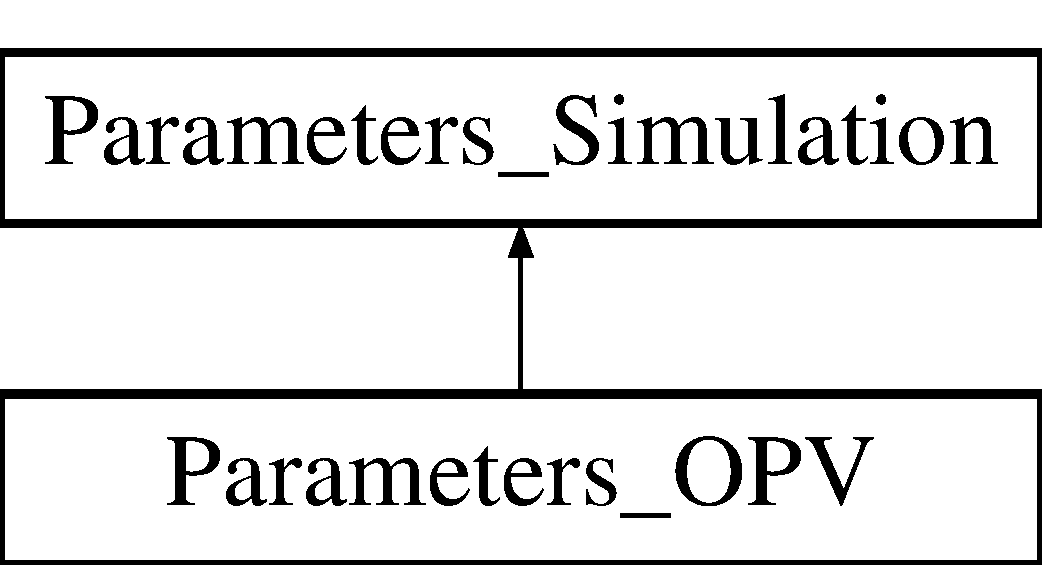
\includegraphics[height=2.000000cm]{struct_parameters___simulation}
\end{center}
\end{figure}
\subsection*{Public Attributes}
\begin{DoxyCompactItemize}
\item 
\mbox{\Hypertarget{struct_parameters___simulation_afde5aaac6f3cd226249cb9646a4c8a4b}\label{struct_parameters___simulation_afde5aaac6f3cd226249cb9646a4c8a4b}} 
bool \hyperlink{struct_parameters___simulation_afde5aaac6f3cd226249cb9646a4c8a4b}{Enable\+\_\+logging}
\begin{DoxyCompactList}\small\item\em Determines whether logging to a logfile during the simulation will be enabled or not. \end{DoxyCompactList}\item 
\mbox{\Hypertarget{struct_parameters___simulation_a5624782454dd99271ad94923f53866b4}\label{struct_parameters___simulation_a5624782454dd99271ad94923f53866b4}} 
bool \hyperlink{struct_parameters___simulation_a5624782454dd99271ad94923f53866b4}{Enable\+\_\+periodic\+\_\+x}
\begin{DoxyCompactList}\small\item\em Determines whether the x-\/direction periodic boundary conditions will be enabled or not in the \hyperlink{class_lattice}{Lattice}. \end{DoxyCompactList}\item 
\mbox{\Hypertarget{struct_parameters___simulation_a1c3d79a4dcf194f884e8a3d346c2261a}\label{struct_parameters___simulation_a1c3d79a4dcf194f884e8a3d346c2261a}} 
bool \hyperlink{struct_parameters___simulation_a1c3d79a4dcf194f884e8a3d346c2261a}{Enable\+\_\+periodic\+\_\+y}
\begin{DoxyCompactList}\small\item\em Determines whether the y-\/direction periodic boundary conditions will be enabled or not in the \hyperlink{class_lattice}{Lattice}. \end{DoxyCompactList}\item 
\mbox{\Hypertarget{struct_parameters___simulation_a0d318f1a9eb75fa909b4ae8266696be1}\label{struct_parameters___simulation_a0d318f1a9eb75fa909b4ae8266696be1}} 
bool \hyperlink{struct_parameters___simulation_a0d318f1a9eb75fa909b4ae8266696be1}{Enable\+\_\+periodic\+\_\+z}
\begin{DoxyCompactList}\small\item\em Determines whether the z-\/direction periodic boundary conditions will be enabled or not in the \hyperlink{class_lattice}{Lattice}. \end{DoxyCompactList}\item 
\mbox{\Hypertarget{struct_parameters___simulation_a038f418e1b2e4fec3fc6a8336f8b23de}\label{struct_parameters___simulation_a038f418e1b2e4fec3fc6a8336f8b23de}} 
int \hyperlink{struct_parameters___simulation_a038f418e1b2e4fec3fc6a8336f8b23de}{Length}
\begin{DoxyCompactList}\small\item\em Defines the desired x-\/direction size of the \hyperlink{class_lattice}{Lattice}. \end{DoxyCompactList}\item 
\mbox{\Hypertarget{struct_parameters___simulation_aab42f7eb6b5ec1916475d9022ed5165f}\label{struct_parameters___simulation_aab42f7eb6b5ec1916475d9022ed5165f}} 
int \hyperlink{struct_parameters___simulation_aab42f7eb6b5ec1916475d9022ed5165f}{Width}
\begin{DoxyCompactList}\small\item\em Defines the desired y-\/direction size of the \hyperlink{class_lattice}{Lattice}. \end{DoxyCompactList}\item 
\mbox{\Hypertarget{struct_parameters___simulation_aa1ffb86ac22065dbbb58196db95b3199}\label{struct_parameters___simulation_aa1ffb86ac22065dbbb58196db95b3199}} 
int \hyperlink{struct_parameters___simulation_aa1ffb86ac22065dbbb58196db95b3199}{Height}
\begin{DoxyCompactList}\small\item\em Defines the desired z-\/direction size of the \hyperlink{class_lattice}{Lattice}. \end{DoxyCompactList}\item 
\mbox{\Hypertarget{struct_parameters___simulation_ab5dda6868bc9359d97a614f027734349}\label{struct_parameters___simulation_ab5dda6868bc9359d97a614f027734349}} 
double \hyperlink{struct_parameters___simulation_ab5dda6868bc9359d97a614f027734349}{Unit\+\_\+size}
\begin{DoxyCompactList}\small\item\em Defines the desired resolution of the \hyperlink{class_lattice}{Lattice} in units of nm. \end{DoxyCompactList}\item 
\mbox{\Hypertarget{struct_parameters___simulation_aad5bdf64239620d1b214c49532dba743}\label{struct_parameters___simulation_aad5bdf64239620d1b214c49532dba743}} 
int \hyperlink{struct_parameters___simulation_aad5bdf64239620d1b214c49532dba743}{Temperature}
\begin{DoxyCompactList}\small\item\em Defines the desired temperature of the simulation in Kelvin. \end{DoxyCompactList}\item 
\mbox{\Hypertarget{struct_parameters___simulation_af55371ca9e7027e799f5be46e40eacc1}\label{struct_parameters___simulation_af55371ca9e7027e799f5be46e40eacc1}} 
int \hyperlink{struct_parameters___simulation_af55371ca9e7027e799f5be46e40eacc1}{Recalc\+\_\+cutoff}
\begin{DoxyCompactList}\small\item\em Defines the desired event recalculation cutoff radius for the simulation in nm. \end{DoxyCompactList}\item 
\mbox{\Hypertarget{struct_parameters___simulation_aa491c1f8ca5045b4cc9c8bbfcb930024}\label{struct_parameters___simulation_aa491c1f8ca5045b4cc9c8bbfcb930024}} 
std\+::ofstream $\ast$ \hyperlink{struct_parameters___simulation_aa491c1f8ca5045b4cc9c8bbfcb930024}{Logfile}
\begin{DoxyCompactList}\small\item\em Defines the desired output file stream pointer to the logfile. \end{DoxyCompactList}\end{DoxyCompactItemize}


\subsection{Detailed Description}
This struct contains all of the main input parameters needed by the \hyperlink{class_simulation}{Simulation} class. 

\begin{DoxyCopyright}{Copyright}
M\+IT License. For more information, see the L\+I\+C\+E\+N\+SE file that accompanies this software package. 
\end{DoxyCopyright}
\begin{DoxyAuthor}{Author}
Michael C. Heiber 
\end{DoxyAuthor}
\begin{DoxyDate}{Date}
2017 
\end{DoxyDate}


The documentation for this struct was generated from the following file\+:\begin{DoxyCompactItemize}
\item 
K\+M\+C\+\_\+\+Lattice/Simulation.\+h\end{DoxyCompactItemize}

\hypertarget{class_polaron}{}\section{Polaron Class Reference}
\label{class_polaron}\index{Polaron@{Polaron}}
Inheritance diagram for Polaron\+:\begin{figure}[H]
\begin{center}
\leavevmode
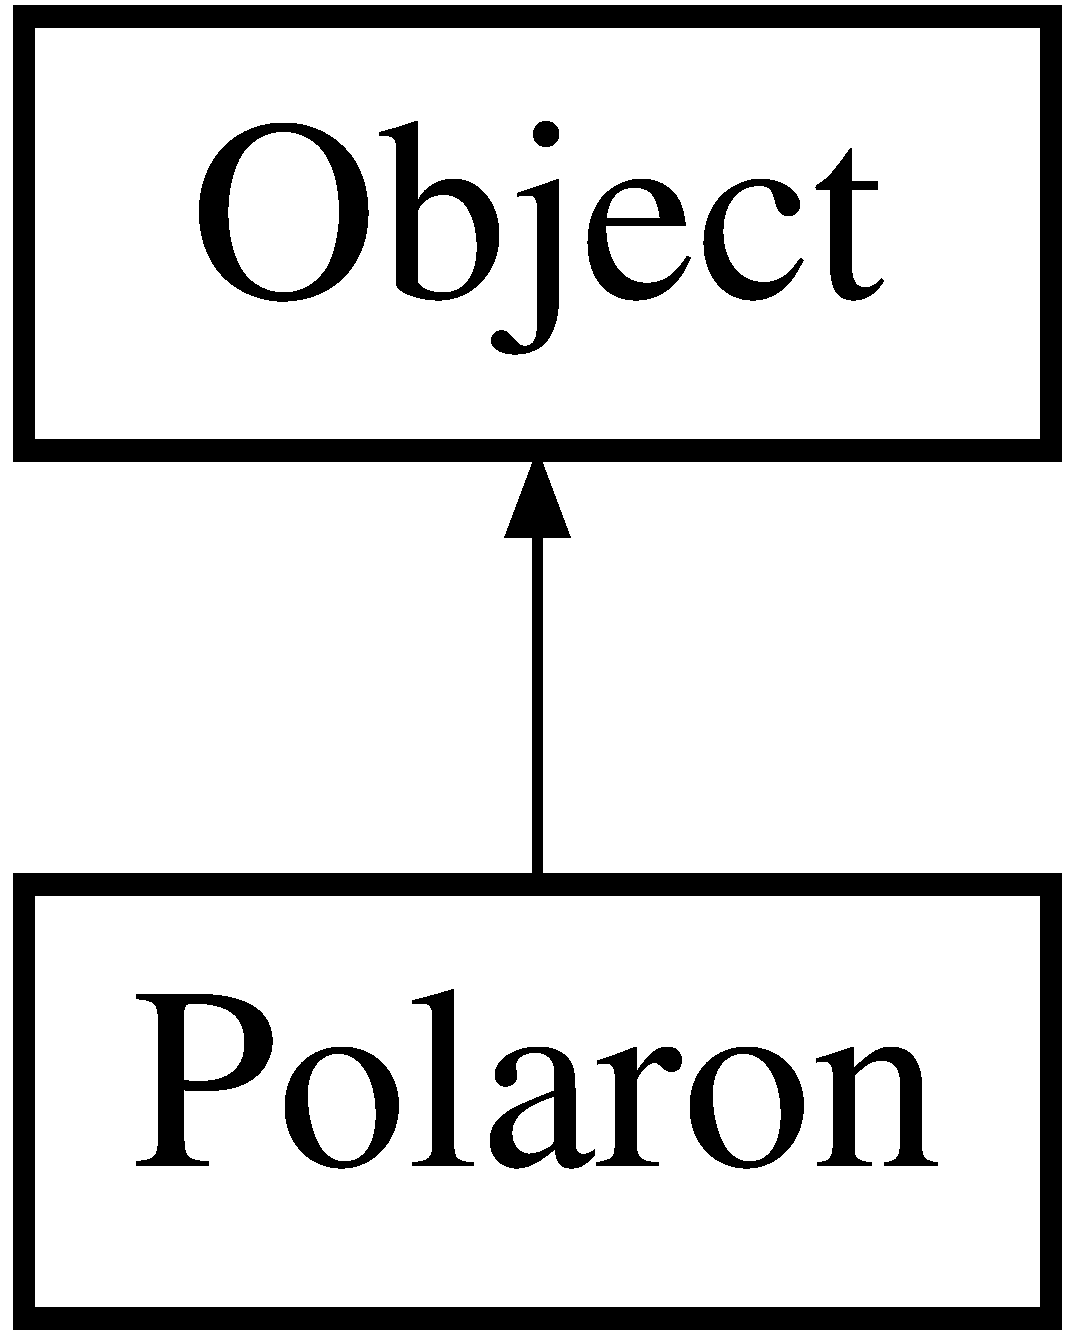
\includegraphics[height=2.000000cm]{class_polaron}
\end{center}
\end{figure}
\subsection*{Public Member Functions}
\begin{DoxyCompactItemize}
\item 
\mbox{\Hypertarget{class_polaron_a7392b742eec8c5bf4438198901c570a9}\label{class_polaron_a7392b742eec8c5bf4438198901c570a9}} 
{\bfseries Polaron} (const double time, const int tag\+\_\+num, const \hyperlink{struct_coords}{Coords} \&start\+\_\+coords, const bool polaron\+\_\+charge)
\item 
\mbox{\Hypertarget{class_polaron_a41c1a9b0b23a35e6ff765c8168a9fb6f}\label{class_polaron_a41c1a9b0b23a35e6ff765c8168a9fb6f}} 
bool {\bfseries get\+Charge} () const
\item 
std\+::string \hyperlink{class_polaron_ab30575f6248183c9dab4d257df2f91fc}{get\+Name} () const
\begin{DoxyCompactList}\small\item\em Gets the name of the \hyperlink{class_object}{Object} class. \end{DoxyCompactList}\end{DoxyCompactItemize}
\subsection*{Static Public Attributes}
\begin{DoxyCompactItemize}
\item 
\mbox{\Hypertarget{class_polaron_aee580c6a3921395abe02c3be1b55339a}\label{class_polaron_aee580c6a3921395abe02c3be1b55339a}} 
static const std\+::string {\bfseries name} = \char`\"{}Polaron\char`\"{}
\end{DoxyCompactItemize}


\subsection{Member Function Documentation}
\mbox{\Hypertarget{class_polaron_ab30575f6248183c9dab4d257df2f91fc}\label{class_polaron_ab30575f6248183c9dab4d257df2f91fc}} 
\index{Polaron@{Polaron}!get\+Name@{get\+Name}}
\index{get\+Name@{get\+Name}!Polaron@{Polaron}}
\subsubsection{\texorpdfstring{get\+Name()}{getName()}}
{\footnotesize\ttfamily std\+::string Polaron\+::get\+Name (\begin{DoxyParamCaption}{ }\end{DoxyParamCaption}) const\hspace{0.3cm}{\ttfamily [inline]}, {\ttfamily [virtual]}}



Gets the name of the \hyperlink{class_object}{Object} class. 

\begin{DoxyReturn}{Returns}
\char`\"{}\+Object\char`\"{} when called on the base class. 
\end{DoxyReturn}


Reimplemented from \hyperlink{class_object_ade517616d51cd9ab581ec5afeb37b313}{Object}.



The documentation for this class was generated from the following files\+:\begin{DoxyCompactItemize}
\item 
Polaron.\+h\item 
Polaron.\+cpp\end{DoxyCompactItemize}

\hypertarget{class_polaron___extraction}{}\section{Polaron\+\_\+\+Extraction Class Reference}
\label{class_polaron___extraction}\index{Polaron\+\_\+\+Extraction@{Polaron\+\_\+\+Extraction}}
Inheritance diagram for Polaron\+\_\+\+Extraction\+:\begin{figure}[H]
\begin{center}
\leavevmode
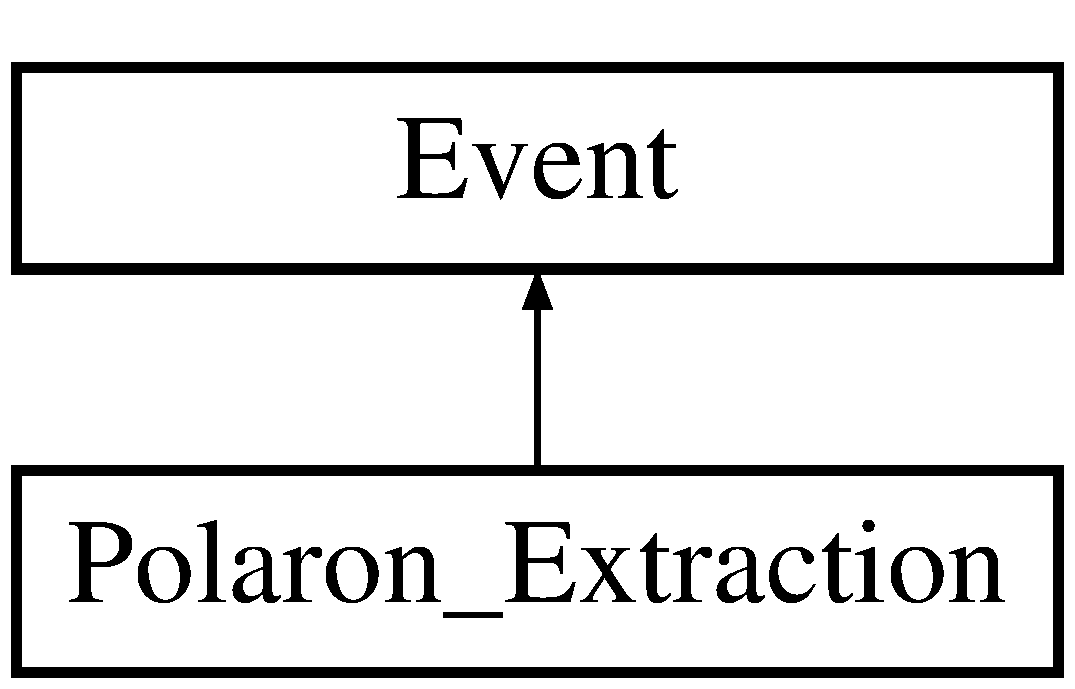
\includegraphics[height=2.000000cm]{class_polaron___extraction}
\end{center}
\end{figure}
\subsection*{Public Member Functions}
\begin{DoxyCompactItemize}
\item 
\mbox{\Hypertarget{class_polaron___extraction_afd2c6e23a838dfb3ea788f1ec3fb360a}\label{class_polaron___extraction_afd2c6e23a838dfb3ea788f1ec3fb360a}} 
void {\bfseries calculate\+Execution\+Time} (const double prefactor, const double localization, const double distance, const double E\+\_\+delta, \hyperlink{class_simulation}{Simulation} $\ast$sim\+\_\+ptr)
\item 
std\+::string \hyperlink{class_polaron___extraction_a30cc8c9489f69e24feda42c035adc9cf}{get\+Name} () const
\begin{DoxyCompactList}\small\item\em Gets the name of event class. \end{DoxyCompactList}\end{DoxyCompactItemize}
\subsection*{Static Public Attributes}
\begin{DoxyCompactItemize}
\item 
\mbox{\Hypertarget{class_polaron___extraction_a35aa28eda2227a38857f42685597eda2}\label{class_polaron___extraction_a35aa28eda2227a38857f42685597eda2}} 
static const std\+::string {\bfseries name} = \char`\"{}Polaron Extraction\char`\"{}
\end{DoxyCompactItemize}


\subsection{Member Function Documentation}
\mbox{\Hypertarget{class_polaron___extraction_a30cc8c9489f69e24feda42c035adc9cf}\label{class_polaron___extraction_a30cc8c9489f69e24feda42c035adc9cf}} 
\index{Polaron\+\_\+\+Extraction@{Polaron\+\_\+\+Extraction}!get\+Name@{get\+Name}}
\index{get\+Name@{get\+Name}!Polaron\+\_\+\+Extraction@{Polaron\+\_\+\+Extraction}}
\subsubsection{\texorpdfstring{get\+Name()}{getName()}}
{\footnotesize\ttfamily std\+::string Polaron\+\_\+\+Extraction\+::get\+Name (\begin{DoxyParamCaption}{ }\end{DoxyParamCaption}) const\hspace{0.3cm}{\ttfamily [inline]}, {\ttfamily [virtual]}}



Gets the name of event class. 

\begin{DoxyReturn}{Returns}
\char`\"{}\+Event\char`\"{} when called on the base class. 
\end{DoxyReturn}


Reimplemented from \hyperlink{class_event_a8c38a406d844d05eac1ef007bad2487f}{Event}.



The documentation for this class was generated from the following files\+:\begin{DoxyCompactItemize}
\item 
Polaron.\+h\item 
Polaron.\+cpp\end{DoxyCompactItemize}

\hypertarget{class_polaron___hop}{}\section{Polaron\+\_\+\+Hop Class Reference}
\label{class_polaron___hop}\index{Polaron\+\_\+\+Hop@{Polaron\+\_\+\+Hop}}
Inheritance diagram for Polaron\+\_\+\+Hop\+:\begin{figure}[H]
\begin{center}
\leavevmode
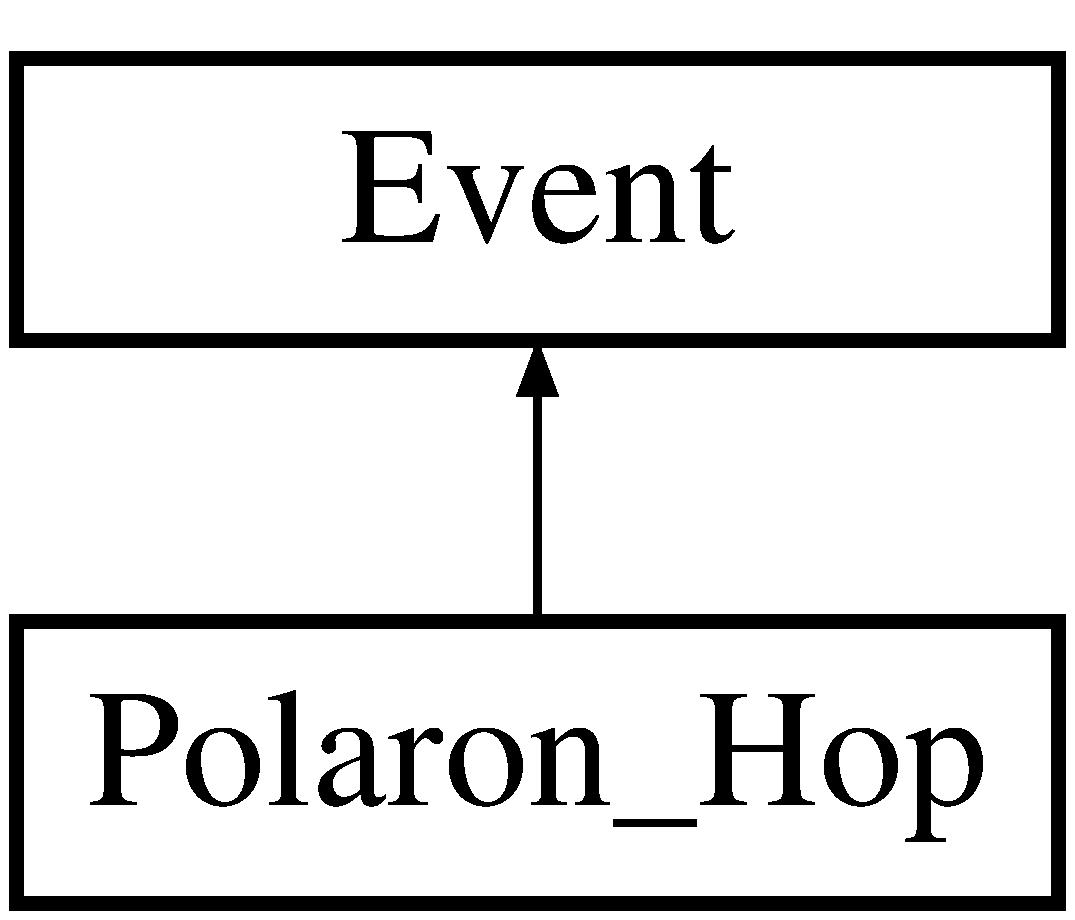
\includegraphics[height=2.000000cm]{class_polaron___hop}
\end{center}
\end{figure}
\subsection*{Public Member Functions}
\begin{DoxyCompactItemize}
\item 
\mbox{\Hypertarget{class_polaron___hop_a045872c8934bc0a93245f4fecb4396ed}\label{class_polaron___hop_a045872c8934bc0a93245f4fecb4396ed}} 
void {\bfseries calculate\+Execution\+Time} (const double prefactor, const double localization, const double distance, const double E\+\_\+delta, \hyperlink{class_simulation}{Simulation} $\ast$sim\+\_\+ptr)
\item 
\mbox{\Hypertarget{class_polaron___hop_a338a825324a7901a8a6b3d1496c7741d}\label{class_polaron___hop_a338a825324a7901a8a6b3d1496c7741d}} 
void {\bfseries calculate\+Execution\+Time} (const double prefactor, const double localization, const double distance, const double E\+\_\+delta, const double reorganization, \hyperlink{class_simulation}{Simulation} $\ast$sim\+\_\+ptr)
\item 
std\+::string \hyperlink{class_polaron___hop_adbb1a3f86bd6a2dd21849bfec5598d70}{get\+Name} () const
\begin{DoxyCompactList}\small\item\em Gets the name of event class. \end{DoxyCompactList}\end{DoxyCompactItemize}
\subsection*{Static Public Attributes}
\begin{DoxyCompactItemize}
\item 
\mbox{\Hypertarget{class_polaron___hop_abcfa4d47e99311d95dd2284bd67cc95a}\label{class_polaron___hop_abcfa4d47e99311d95dd2284bd67cc95a}} 
static const std\+::string {\bfseries name} = \char`\"{}Polaron Hop\char`\"{}
\end{DoxyCompactItemize}


\subsection{Member Function Documentation}
\mbox{\Hypertarget{class_polaron___hop_adbb1a3f86bd6a2dd21849bfec5598d70}\label{class_polaron___hop_adbb1a3f86bd6a2dd21849bfec5598d70}} 
\index{Polaron\+\_\+\+Hop@{Polaron\+\_\+\+Hop}!get\+Name@{get\+Name}}
\index{get\+Name@{get\+Name}!Polaron\+\_\+\+Hop@{Polaron\+\_\+\+Hop}}
\subsubsection{\texorpdfstring{get\+Name()}{getName()}}
{\footnotesize\ttfamily std\+::string Polaron\+\_\+\+Hop\+::get\+Name (\begin{DoxyParamCaption}{ }\end{DoxyParamCaption}) const\hspace{0.3cm}{\ttfamily [inline]}, {\ttfamily [virtual]}}



Gets the name of event class. 

\begin{DoxyReturn}{Returns}
\char`\"{}\+Event\char`\"{} when called on the base class. 
\end{DoxyReturn}


Reimplemented from \hyperlink{class_event_a8c38a406d844d05eac1ef007bad2487f}{Event}.



The documentation for this class was generated from the following files\+:\begin{DoxyCompactItemize}
\item 
Polaron.\+h\item 
Polaron.\+cpp\end{DoxyCompactItemize}

\hypertarget{class_polaron___recombination}{}\section{Polaron\+\_\+\+Recombination Class Reference}
\label{class_polaron___recombination}\index{Polaron\+\_\+\+Recombination@{Polaron\+\_\+\+Recombination}}
Inheritance diagram for Polaron\+\_\+\+Recombination\+:\begin{figure}[H]
\begin{center}
\leavevmode
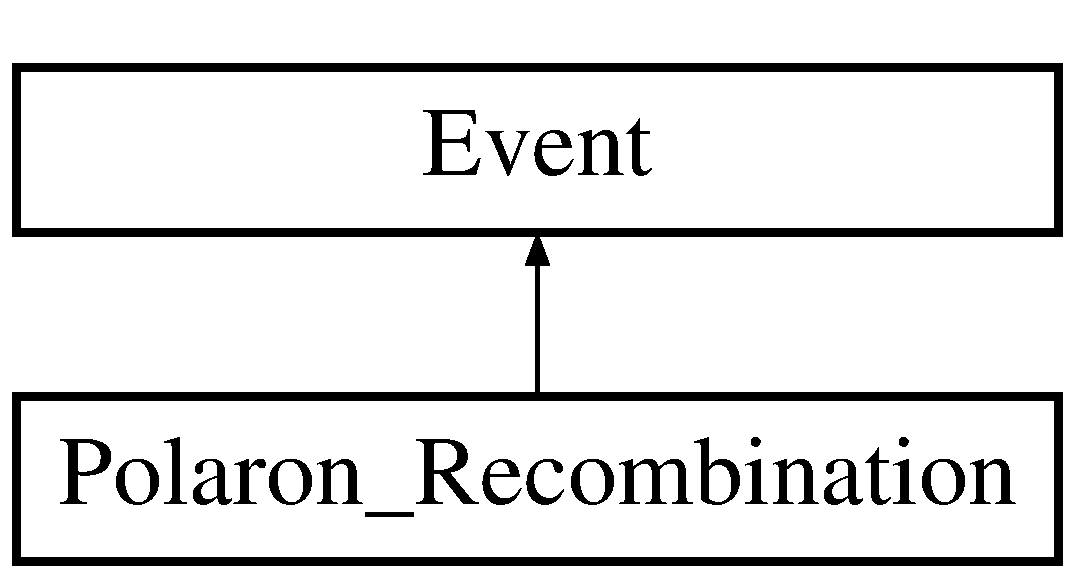
\includegraphics[height=2.000000cm]{class_polaron___recombination}
\end{center}
\end{figure}
\subsection*{Public Member Functions}
\begin{DoxyCompactItemize}
\item 
\mbox{\Hypertarget{class_polaron___recombination_ab987d4755177c0a698087c79a1347bfe}\label{class_polaron___recombination_ab987d4755177c0a698087c79a1347bfe}} 
void {\bfseries calculate\+Execution\+Time} (const double prefactor, const double localization, const double distance, const double E\+\_\+delta, \hyperlink{class_simulation}{Simulation} $\ast$sim\+\_\+ptr)
\item 
\mbox{\Hypertarget{class_polaron___recombination_ac7d9302d957a3e3b08d58d5b39332df8}\label{class_polaron___recombination_ac7d9302d957a3e3b08d58d5b39332df8}} 
void {\bfseries calculate\+Execution\+Time} (const double prefactor, const double localization, const double distance, const double E\+\_\+delta, const double reorganization, \hyperlink{class_simulation}{Simulation} $\ast$sim\+\_\+ptr)
\item 
std\+::string \hyperlink{class_polaron___recombination_a0075250a377d6fccb8f64e4d173c9041}{get\+Name} () const
\begin{DoxyCompactList}\small\item\em Gets the name of event class. \end{DoxyCompactList}\end{DoxyCompactItemize}
\subsection*{Static Public Attributes}
\begin{DoxyCompactItemize}
\item 
\mbox{\Hypertarget{class_polaron___recombination_aa7a004a1e87bccff00a28dde96df78ba}\label{class_polaron___recombination_aa7a004a1e87bccff00a28dde96df78ba}} 
static const std\+::string {\bfseries name} = \char`\"{}Polaron Recombination\char`\"{}
\end{DoxyCompactItemize}


\subsection{Member Function Documentation}
\mbox{\Hypertarget{class_polaron___recombination_a0075250a377d6fccb8f64e4d173c9041}\label{class_polaron___recombination_a0075250a377d6fccb8f64e4d173c9041}} 
\index{Polaron\+\_\+\+Recombination@{Polaron\+\_\+\+Recombination}!get\+Name@{get\+Name}}
\index{get\+Name@{get\+Name}!Polaron\+\_\+\+Recombination@{Polaron\+\_\+\+Recombination}}
\subsubsection{\texorpdfstring{get\+Name()}{getName()}}
{\footnotesize\ttfamily std\+::string Polaron\+\_\+\+Recombination\+::get\+Name (\begin{DoxyParamCaption}{ }\end{DoxyParamCaption}) const\hspace{0.3cm}{\ttfamily [inline]}, {\ttfamily [virtual]}}



Gets the name of event class. 

\begin{DoxyReturn}{Returns}
\char`\"{}\+Event\char`\"{} when called on the base class. 
\end{DoxyReturn}


Reimplemented from \hyperlink{class_event_a8c38a406d844d05eac1ef007bad2487f}{Event}.



The documentation for this class was generated from the following files\+:\begin{DoxyCompactItemize}
\item 
Polaron.\+h\item 
Polaron.\+cpp\end{DoxyCompactItemize}

\hypertarget{class_simulation}{}\section{Simulation Class Reference}
\label{class_simulation}\index{Simulation@{Simulation}}


This abstract base class contains the basic properties of a K\+MC simulation and the functions needed to interact with it.  




{\ttfamily \#include $<$Simulation.\+h$>$}

Inheritance diagram for Simulation\+:\begin{figure}[H]
\begin{center}
\leavevmode
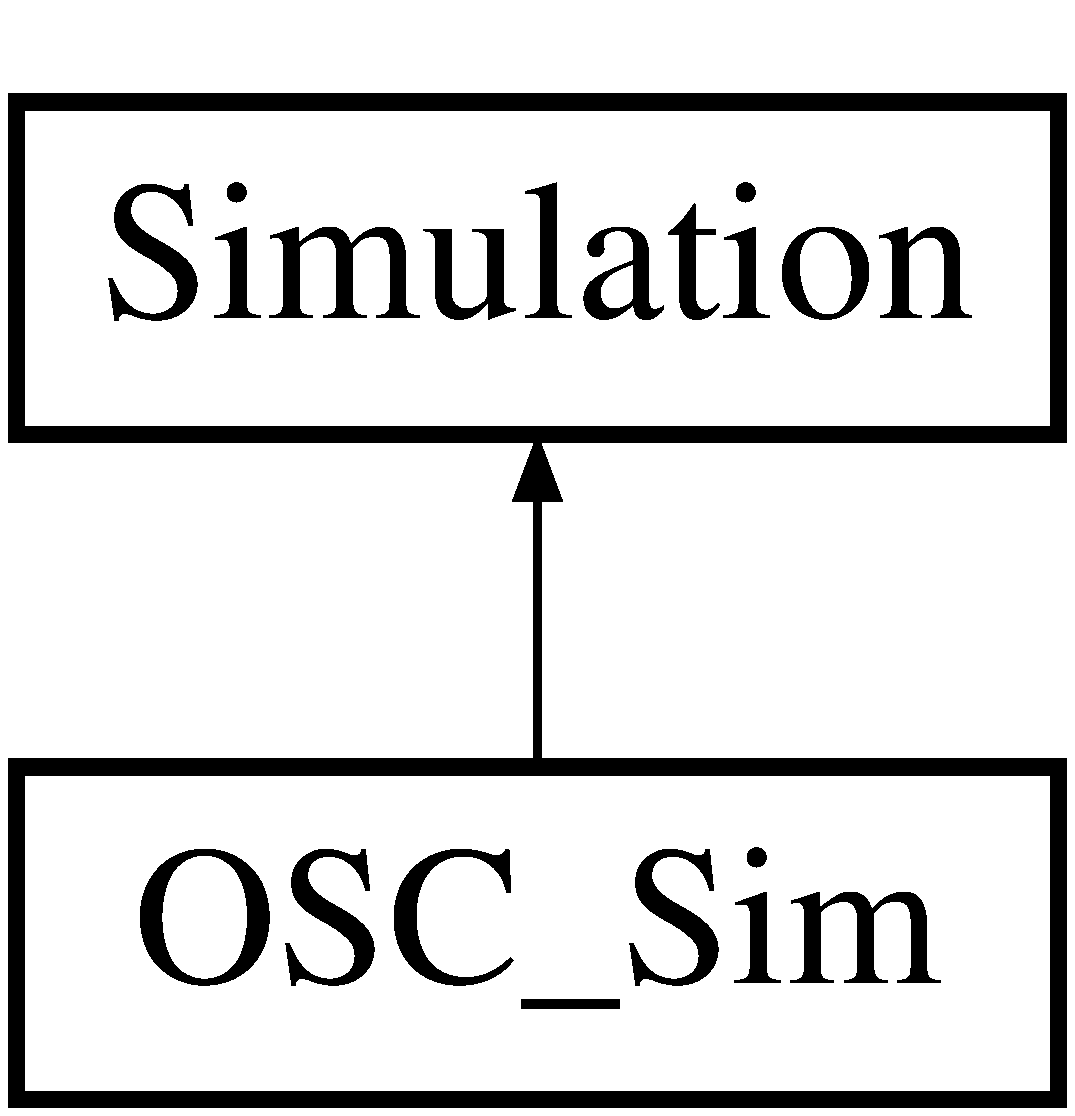
\includegraphics[height=2.000000cm]{class_simulation}
\end{center}
\end{figure}
\subsection*{Public Member Functions}
\begin{DoxyCompactItemize}
\item 
\mbox{\Hypertarget{class_simulation_a80fad3f57dfaf195a36f7bc49bc88279}\label{class_simulation_a80fad3f57dfaf195a36f7bc49bc88279}} 
virtual \hyperlink{class_simulation_a80fad3f57dfaf195a36f7bc49bc88279}{$\sim$\+Simulation} ()
\begin{DoxyCompactList}\small\item\em Default virtual destructor needed by the base class. \end{DoxyCompactList}\item 
\hyperlink{class_simulation_a5b224cc5b36bcc8eb29689aff223de41}{Simulation} ()
\begin{DoxyCompactList}\small\item\em Default constructor that creates an empty \hyperlink{class_simulation}{Simulation} object. \end{DoxyCompactList}\item 
void \hyperlink{class_simulation_af88e5e0634b373ba28f1dd87670725a6}{init} (const \hyperlink{struct_parameters___simulation}{Parameters\+\_\+\+Simulation} \&params, const int id)
\begin{DoxyCompactList}\small\item\em Initializes the \hyperlink{class_simulation}{Simulation} object using the provided \hyperlink{struct_parameters___simulation}{Parameters\+\_\+\+Simulation} struct containing the input parameters. \end{DoxyCompactList}\item 
virtual bool \hyperlink{class_simulation_af69bb46977a3a0084214a194c888e16c}{check\+Finished} () const =0
\begin{DoxyCompactList}\small\item\em Checks whether or not the simulation has finished. \end{DoxyCompactList}\item 
virtual bool \hyperlink{class_simulation_a48e9e82f9dac1acec5d063a9f6f6115e}{execute\+Next\+Event} ()=0
\begin{DoxyCompactList}\small\item\em Executes the next event in the simulation. \end{DoxyCompactList}\item 
int \hyperlink{class_simulation_a7d88f18a1ba988d7e77b8be8de5b10d1}{get\+N\+\_\+events} () const
\begin{DoxyCompactList}\small\item\em Gets the number of events that are currently in the event list. \end{DoxyCompactList}\item 
\mbox{\Hypertarget{class_simulation_a52cb5564151421cbefaca56357738de7}\label{class_simulation_a52cb5564151421cbefaca56357738de7}} 
long int \hyperlink{class_simulation_a52cb5564151421cbefaca56357738de7}{get\+N\+\_\+events\+\_\+executed} () const
\begin{DoxyCompactList}\small\item\em Gets the number of events that have been executed in the simulation. \end{DoxyCompactList}\item 
int \hyperlink{class_simulation_aff40f268758bd9a0f390a649fc45c05e}{get\+Id} () const
\begin{DoxyCompactList}\small\item\em Gets the processor ID number for the processor that is running the simulation. \end{DoxyCompactList}\item 
\mbox{\Hypertarget{class_simulation_ac00bce7c792fb67a75395c46c03efe0a}\label{class_simulation_ac00bce7c792fb67a75395c46c03efe0a}} 
int \hyperlink{class_simulation_ac00bce7c792fb67a75395c46c03efe0a}{get\+Temp} () const
\begin{DoxyCompactList}\small\item\em Gets the value of the temperature parameter. \end{DoxyCompactList}\item 
\mbox{\Hypertarget{class_simulation_a391ac262089c8bda8e76ce930b1db88b}\label{class_simulation_a391ac262089c8bda8e76ce930b1db88b}} 
double \hyperlink{class_simulation_a391ac262089c8bda8e76ce930b1db88b}{get\+Time} () const
\begin{DoxyCompactList}\small\item\em Get the current simulation time in units of seconds. \end{DoxyCompactList}\item 
bool \hyperlink{class_simulation_ac7c8a49a4cc506b850891480e0aae512}{is\+Logging\+Enabled} () const
\begin{DoxyCompactList}\small\item\em Checks whether or not logging is enabled. \end{DoxyCompactList}\item 
\mbox{\Hypertarget{class_simulation_a938de951b2766c6fb2b00cf9714caffa}\label{class_simulation_a938de951b2766c6fb2b00cf9714caffa}} 
double \hyperlink{class_simulation_a938de951b2766c6fb2b00cf9714caffa}{rand01} ()
\begin{DoxyCompactList}\small\item\em Generates a uniform random number from 0 to 1, not including 0. \end{DoxyCompactList}\item 
void \hyperlink{class_simulation_a1a825b9da67da43104137662694655bd}{set\+Generator\+Seed} (const int seed)
\begin{DoxyCompactList}\small\item\em Sets the random number generator seed. \end{DoxyCompactList}\end{DoxyCompactItemize}
\subsection*{Protected Member Functions}
\begin{DoxyCompactItemize}
\item 
std\+::list$<$ \hyperlink{class_event}{Event} $\ast$ $>$\+::iterator \hyperlink{class_simulation_a4b84249d359723e00ec4ae77164c8b7d}{add\+Event} (\hyperlink{class_event}{Event} $\ast$event\+\_\+ptr)
\begin{DoxyCompactList}\small\item\em Adds a pointer to an \hyperlink{class_event}{Event} object to the event list and returns the iterator to its position in the list. \end{DoxyCompactList}\item 
void \hyperlink{class_simulation_a1e0f43c4e11eda5486054c250f4de08f}{add\+Object} (\hyperlink{class_object}{Object} $\ast$object\+\_\+ptr)
\begin{DoxyCompactList}\small\item\em Adds a pointer to an \hyperlink{class_object}{Object} object to the object list. \end{DoxyCompactList}\item 
std\+::list$<$ \hyperlink{class_event}{Event} $\ast$ $>$\+::iterator \hyperlink{class_simulation_a401d40509ba367a28702873a0d65188d}{choose\+Next\+Event} ()
\begin{DoxyCompactList}\small\item\em Searches the event list and determines which event will be executed next. \end{DoxyCompactList}\item 
std\+::vector$<$ \hyperlink{class_object}{Object} $\ast$ $>$ \hyperlink{class_simulation_aa6501dc60b4a3981f6ca44cec861364a}{find\+Recalc\+Neighbors} (const \hyperlink{struct_coords}{Coords} \&coords) const
\begin{DoxyCompactList}\small\item\em Locates and returns a vector of pointers to all \hyperlink{class_object}{Object} objects near the input coordinates within the Recalc\+\_\+cutoff radius. \end{DoxyCompactList}\item 
\mbox{\Hypertarget{class_simulation_a620684b9ac1fb07344c4c2237ed9f352}\label{class_simulation_a620684b9ac1fb07344c4c2237ed9f352}} 
std\+::vector$<$ \hyperlink{class_object}{Object} $\ast$ $>$ \hyperlink{class_simulation_a620684b9ac1fb07344c4c2237ed9f352}{get\+All\+Object\+Ptrs} () const
\begin{DoxyCompactList}\small\item\em Returns a vector of pointers to all \hyperlink{class_object}{Object} objects in the simulation. \end{DoxyCompactList}\item 
void \hyperlink{class_simulation_a7b10f51640088366d0d1278361817e8d}{move\+Object} (\hyperlink{class_object}{Object} $\ast$object\+\_\+ptr, const \hyperlink{struct_coords}{Coords} \&dest\+\_\+coords)
\begin{DoxyCompactList}\small\item\em Moves the designated object to the designated destination coordinates. \end{DoxyCompactList}\item 
void \hyperlink{class_simulation_a3a4808231d4760f0ab30ea39b6a67e8c}{remove\+Event} (\hyperlink{class_event}{Event} $\ast$event\+\_\+ptr)
\begin{DoxyCompactList}\small\item\em Removes an \hyperlink{class_event}{Event} pointer from the event list. \end{DoxyCompactList}\item 
void \hyperlink{class_simulation_a39da17feb9b487c05c9a834def44972f}{remove\+Object} (\hyperlink{class_object}{Object} $\ast$object\+\_\+ptr)
\begin{DoxyCompactList}\small\item\em Removes the \hyperlink{class_object}{Object} pointer from the base simulation class. \end{DoxyCompactList}\item 
void \hyperlink{class_simulation_a4490fc0d8bb8a36b0ff581148ab85a14}{set\+Event} (const std\+::list$<$ \hyperlink{class_event}{Event} $\ast$$>$\+::iterator event\+\_\+it, \hyperlink{class_event}{Event} $\ast$event\+\_\+ptr)
\begin{DoxyCompactList}\small\item\em Overwrites the \hyperlink{class_event}{Event} pointer in the event list indicated by the input iterator to the input \hyperlink{class_event}{Event} pointer. \end{DoxyCompactList}\item 
void \hyperlink{class_simulation_a1affa7d0725c3d10663095619dcb9208}{update\+Time} (const double input\+\_\+time)
\begin{DoxyCompactList}\small\item\em Updates the simulation time with the input time. \end{DoxyCompactList}\end{DoxyCompactItemize}
\subsection*{Protected Attributes}
\begin{DoxyCompactItemize}
\item 
\mbox{\Hypertarget{class_simulation_a80d697e885e6fa3a0ab688b25b366194}\label{class_simulation_a80d697e885e6fa3a0ab688b25b366194}} 
std\+::mt19937 \hyperlink{class_simulation_a80d697e885e6fa3a0ab688b25b366194}{gen}
\begin{DoxyCompactList}\small\item\em Mersenne Twister random number generator. \end{DoxyCompactList}\item 
\mbox{\Hypertarget{class_simulation_a741321a0bbc89d51b969abda469e6f96}\label{class_simulation_a741321a0bbc89d51b969abda469e6f96}} 
std\+::ofstream $\ast$ \hyperlink{class_simulation_a741321a0bbc89d51b969abda469e6f96}{Logfile}
\begin{DoxyCompactList}\small\item\em Pointer to an output file stream that is used to print log messages to a logfile when logging is enabled. \end{DoxyCompactList}\item 
\mbox{\Hypertarget{class_simulation_afb2cf4feeb4d8292eeba8f9ef393c6a4}\label{class_simulation_afb2cf4feeb4d8292eeba8f9ef393c6a4}} 
\hyperlink{class_lattice}{Lattice} \hyperlink{class_simulation_afb2cf4feeb4d8292eeba8f9ef393c6a4}{lattice}
\begin{DoxyCompactList}\small\item\em The \hyperlink{class_lattice}{Lattice} object represents a three-\/dimensional lattice, its boundary conditions, and its occupancy. \end{DoxyCompactList}\item 
\mbox{\Hypertarget{class_simulation_a7f4615a7898fb83d09be5e7fad92bb47}\label{class_simulation_a7f4615a7898fb83d09be5e7fad92bb47}} 
bool \hyperlink{class_simulation_a7f4615a7898fb83d09be5e7fad92bb47}{Error\+\_\+found} = false
\begin{DoxyCompactList}\small\item\em The Error\+\_\+found flag indicates whether or not there has been an error during one of the simulation operations. \end{DoxyCompactList}\end{DoxyCompactItemize}


\subsection{Detailed Description}
This abstract base class contains the basic properties of a K\+MC simulation and the functions needed to interact with it. 

This abstract base class must be extended using a derived simulation class. \begin{DoxyCopyright}{Copyright}
M\+IT License. For more information, see the L\+I\+C\+E\+N\+SE file that accompanies this software package. 
\end{DoxyCopyright}
\begin{DoxyAuthor}{Author}
Michael C. Heiber 
\end{DoxyAuthor}
\begin{DoxyDate}{Date}
2017 
\end{DoxyDate}


\subsection{Constructor \& Destructor Documentation}
\mbox{\Hypertarget{class_simulation_a5b224cc5b36bcc8eb29689aff223de41}\label{class_simulation_a5b224cc5b36bcc8eb29689aff223de41}} 
\index{Simulation@{Simulation}!Simulation@{Simulation}}
\index{Simulation@{Simulation}!Simulation@{Simulation}}
\subsubsection{\texorpdfstring{Simulation()}{Simulation()}}
{\footnotesize\ttfamily Simulation\+::\+Simulation (\begin{DoxyParamCaption}{ }\end{DoxyParamCaption})}



Default constructor that creates an empty \hyperlink{class_simulation}{Simulation} object. 

\begin{DoxyWarning}{Warning}
An empty \hyperlink{class_simulation}{Simulation} object should not be used until the init function has been called. 
\end{DoxyWarning}


\subsection{Member Function Documentation}
\mbox{\Hypertarget{class_simulation_a4b84249d359723e00ec4ae77164c8b7d}\label{class_simulation_a4b84249d359723e00ec4ae77164c8b7d}} 
\index{Simulation@{Simulation}!add\+Event@{add\+Event}}
\index{add\+Event@{add\+Event}!Simulation@{Simulation}}
\subsubsection{\texorpdfstring{add\+Event()}{addEvent()}}
{\footnotesize\ttfamily list$<$ \hyperlink{class_event}{Event} $\ast$ $>$\+::iterator Simulation\+::add\+Event (\begin{DoxyParamCaption}\item[{\hyperlink{class_event}{Event} $\ast$}]{event\+\_\+ptr }\end{DoxyParamCaption})\hspace{0.3cm}{\ttfamily [protected]}}



Adds a pointer to an \hyperlink{class_event}{Event} object to the event list and returns the iterator to its position in the list. 


\begin{DoxyParams}{Parameters}
{\em event\+\_\+ptr} & is the input \hyperlink{class_event}{Event} pointer. \\
\hline
\end{DoxyParams}
\begin{DoxyReturn}{Returns}
A list iterator that indicates where in the event list the newly added \hyperlink{class_event}{Event} pointer is located. 
\end{DoxyReturn}
\mbox{\Hypertarget{class_simulation_a1e0f43c4e11eda5486054c250f4de08f}\label{class_simulation_a1e0f43c4e11eda5486054c250f4de08f}} 
\index{Simulation@{Simulation}!add\+Object@{add\+Object}}
\index{add\+Object@{add\+Object}!Simulation@{Simulation}}
\subsubsection{\texorpdfstring{add\+Object()}{addObject()}}
{\footnotesize\ttfamily void Simulation\+::add\+Object (\begin{DoxyParamCaption}\item[{\hyperlink{class_object}{Object} $\ast$}]{object\+\_\+ptr }\end{DoxyParamCaption})\hspace{0.3cm}{\ttfamily [protected]}}



Adds a pointer to an \hyperlink{class_object}{Object} object to the object list. 


\begin{DoxyParams}{Parameters}
{\em object\+\_\+ptr} & is the input \hyperlink{class_object}{Object} pointer. \\
\hline
\end{DoxyParams}
\mbox{\Hypertarget{class_simulation_af69bb46977a3a0084214a194c888e16c}\label{class_simulation_af69bb46977a3a0084214a194c888e16c}} 
\index{Simulation@{Simulation}!check\+Finished@{check\+Finished}}
\index{check\+Finished@{check\+Finished}!Simulation@{Simulation}}
\subsubsection{\texorpdfstring{check\+Finished()}{checkFinished()}}
{\footnotesize\ttfamily virtual bool Simulation\+::check\+Finished (\begin{DoxyParamCaption}{ }\end{DoxyParamCaption}) const\hspace{0.3cm}{\ttfamily [pure virtual]}}



Checks whether or not the simulation has finished. 

This is a pure virtual function in the base class that must be defined by any derived class. \begin{DoxyReturn}{Returns}
true if the simulation is finished. 

false if the simulation is not finished. 
\end{DoxyReturn}


Implemented in \hyperlink{class_o_s_c___sim_ab3e4258c850b48ec02e4d3a88b583115}{O\+S\+C\+\_\+\+Sim}.

\mbox{\Hypertarget{class_simulation_a401d40509ba367a28702873a0d65188d}\label{class_simulation_a401d40509ba367a28702873a0d65188d}} 
\index{Simulation@{Simulation}!choose\+Next\+Event@{choose\+Next\+Event}}
\index{choose\+Next\+Event@{choose\+Next\+Event}!Simulation@{Simulation}}
\subsubsection{\texorpdfstring{choose\+Next\+Event()}{chooseNextEvent()}}
{\footnotesize\ttfamily list$<$ \hyperlink{class_event}{Event} $\ast$ $>$\+::iterator Simulation\+::choose\+Next\+Event (\begin{DoxyParamCaption}{ }\end{DoxyParamCaption})\hspace{0.3cm}{\ttfamily [protected]}}



Searches the event list and determines which event will be executed next. 

Chooses the event that has the smallest execution time. \begin{DoxyReturn}{Returns}
A list iterator points to an \hyperlink{class_event}{Event} pointer in event list that has been selected to be executed next. 
\end{DoxyReturn}
\mbox{\Hypertarget{class_simulation_a48e9e82f9dac1acec5d063a9f6f6115e}\label{class_simulation_a48e9e82f9dac1acec5d063a9f6f6115e}} 
\index{Simulation@{Simulation}!execute\+Next\+Event@{execute\+Next\+Event}}
\index{execute\+Next\+Event@{execute\+Next\+Event}!Simulation@{Simulation}}
\subsubsection{\texorpdfstring{execute\+Next\+Event()}{executeNextEvent()}}
{\footnotesize\ttfamily virtual bool Simulation\+::execute\+Next\+Event (\begin{DoxyParamCaption}{ }\end{DoxyParamCaption})\hspace{0.3cm}{\ttfamily [pure virtual]}}



Executes the next event in the simulation. 

This is a pure virtual function in the base class that must be defined by any derived class. \begin{DoxyReturn}{Returns}
true if the next event is succesfully executed. 

false if execution of the next event is unsuccessful. 
\end{DoxyReturn}


Implemented in \hyperlink{class_o_s_c___sim_a41bdb6368c71e1a3cb0efdc2a55d7869}{O\+S\+C\+\_\+\+Sim}.

\mbox{\Hypertarget{class_simulation_aa6501dc60b4a3981f6ca44cec861364a}\label{class_simulation_aa6501dc60b4a3981f6ca44cec861364a}} 
\index{Simulation@{Simulation}!find\+Recalc\+Neighbors@{find\+Recalc\+Neighbors}}
\index{find\+Recalc\+Neighbors@{find\+Recalc\+Neighbors}!Simulation@{Simulation}}
\subsubsection{\texorpdfstring{find\+Recalc\+Neighbors()}{findRecalcNeighbors()}}
{\footnotesize\ttfamily vector$<$ \hyperlink{class_object}{Object} $\ast$ $>$ Simulation\+::find\+Recalc\+Neighbors (\begin{DoxyParamCaption}\item[{const \hyperlink{struct_coords}{Coords} \&}]{coords }\end{DoxyParamCaption}) const\hspace{0.3cm}{\ttfamily [protected]}}



Locates and returns a vector of pointers to all \hyperlink{class_object}{Object} objects near the input coordinates within the Recalc\+\_\+cutoff radius. 


\begin{DoxyParams}{Parameters}
{\em coords} & is the \hyperlink{struct_coords}{Coords} struct that designates the input coordinates. \\
\hline
\end{DoxyParams}
\begin{DoxyReturn}{Returns}
a vector of \hyperlink{class_object}{Object} pointers. 
\end{DoxyReturn}
\mbox{\Hypertarget{class_simulation_aff40f268758bd9a0f390a649fc45c05e}\label{class_simulation_aff40f268758bd9a0f390a649fc45c05e}} 
\index{Simulation@{Simulation}!get\+Id@{get\+Id}}
\index{get\+Id@{get\+Id}!Simulation@{Simulation}}
\subsubsection{\texorpdfstring{get\+Id()}{getId()}}
{\footnotesize\ttfamily int Simulation\+::get\+Id (\begin{DoxyParamCaption}{ }\end{DoxyParamCaption}) const}



Gets the processor ID number for the processor that is running the simulation. 

This is primarly used with M\+PI to differentiate between different simualtions running on different cores. \mbox{\Hypertarget{class_simulation_a7d88f18a1ba988d7e77b8be8de5b10d1}\label{class_simulation_a7d88f18a1ba988d7e77b8be8de5b10d1}} 
\index{Simulation@{Simulation}!get\+N\+\_\+events@{get\+N\+\_\+events}}
\index{get\+N\+\_\+events@{get\+N\+\_\+events}!Simulation@{Simulation}}
\subsubsection{\texorpdfstring{get\+N\+\_\+events()}{getN\_events()}}
{\footnotesize\ttfamily int Simulation\+::get\+N\+\_\+events (\begin{DoxyParamCaption}{ }\end{DoxyParamCaption}) const}



Gets the number of events that are currently in the event list. 

\begin{DoxyReturn}{Returns}
the size of the events list 
\end{DoxyReturn}
\mbox{\Hypertarget{class_simulation_af88e5e0634b373ba28f1dd87670725a6}\label{class_simulation_af88e5e0634b373ba28f1dd87670725a6}} 
\index{Simulation@{Simulation}!init@{init}}
\index{init@{init}!Simulation@{Simulation}}
\subsubsection{\texorpdfstring{init()}{init()}}
{\footnotesize\ttfamily void Simulation\+::init (\begin{DoxyParamCaption}\item[{const \hyperlink{struct_parameters___simulation}{Parameters\+\_\+\+Simulation} \&}]{params,  }\item[{const int}]{id }\end{DoxyParamCaption})}



Initializes the \hyperlink{class_simulation}{Simulation} object using the provided \hyperlink{struct_parameters___simulation}{Parameters\+\_\+\+Simulation} struct containing the input parameters. 


\begin{DoxyParams}{Parameters}
{\em params} & is a \hyperlink{struct_parameters___simulation}{Parameters\+\_\+\+Simulation} struct that contains all of the required parameters to initialize the \hyperlink{class_simulation}{Simulation} object. \\
\hline
{\em id} & is the processor ID number for the processor that is running the simulation. \\
\hline
\end{DoxyParams}
\mbox{\Hypertarget{class_simulation_ac7c8a49a4cc506b850891480e0aae512}\label{class_simulation_ac7c8a49a4cc506b850891480e0aae512}} 
\index{Simulation@{Simulation}!is\+Logging\+Enabled@{is\+Logging\+Enabled}}
\index{is\+Logging\+Enabled@{is\+Logging\+Enabled}!Simulation@{Simulation}}
\subsubsection{\texorpdfstring{is\+Logging\+Enabled()}{isLoggingEnabled()}}
{\footnotesize\ttfamily bool Simulation\+::is\+Logging\+Enabled (\begin{DoxyParamCaption}{ }\end{DoxyParamCaption}) const}



Checks whether or not logging is enabled. 

This is primarily used for debugging purposes. \begin{DoxyReturn}{Returns}
true if logging is enabled. 

false if logging is disabled. 
\end{DoxyReturn}
\mbox{\Hypertarget{class_simulation_a7b10f51640088366d0d1278361817e8d}\label{class_simulation_a7b10f51640088366d0d1278361817e8d}} 
\index{Simulation@{Simulation}!move\+Object@{move\+Object}}
\index{move\+Object@{move\+Object}!Simulation@{Simulation}}
\subsubsection{\texorpdfstring{move\+Object()}{moveObject()}}
{\footnotesize\ttfamily void Simulation\+::move\+Object (\begin{DoxyParamCaption}\item[{\hyperlink{class_object}{Object} $\ast$}]{object\+\_\+ptr,  }\item[{const \hyperlink{struct_coords}{Coords} \&}]{dest\+\_\+coords }\end{DoxyParamCaption})\hspace{0.3cm}{\ttfamily [protected]}}



Moves the designated object to the designated destination coordinates. 


\begin{DoxyParams}{Parameters}
{\em object\+\_\+ptr} & is an \hyperlink{class_object}{Object} pointer to the object that is to be moved. \\
\hline
{\em dest\+\_\+coords} & is the \hyperlink{struct_coords}{Coords} struct that designates the coordinates where the object is to be moved. \\
\hline
\end{DoxyParams}
\mbox{\Hypertarget{class_simulation_a3a4808231d4760f0ab30ea39b6a67e8c}\label{class_simulation_a3a4808231d4760f0ab30ea39b6a67e8c}} 
\index{Simulation@{Simulation}!remove\+Event@{remove\+Event}}
\index{remove\+Event@{remove\+Event}!Simulation@{Simulation}}
\subsubsection{\texorpdfstring{remove\+Event()}{removeEvent()}}
{\footnotesize\ttfamily void Simulation\+::remove\+Event (\begin{DoxyParamCaption}\item[{\hyperlink{class_event}{Event} $\ast$}]{event\+\_\+ptr }\end{DoxyParamCaption})\hspace{0.3cm}{\ttfamily [protected]}}



Removes an \hyperlink{class_event}{Event} pointer from the event list. 

The \hyperlink{class_event}{Event} objects are allocated and maintained by the derived \hyperlink{class_simulation}{Simulation} class and only the \hyperlink{class_event}{Event} pointers are stored in the base class. Removing the \hyperlink{class_event}{Event} pointer does not delete the \hyperlink{class_event}{Event} from the derived class, it only prevents the event from being executed in future simulation iterations. 
\begin{DoxyParams}{Parameters}
{\em event\+\_\+ptr} & is the \hyperlink{class_event}{Event} pointer to be removed from the simulation. \\
\hline
\end{DoxyParams}
\mbox{\Hypertarget{class_simulation_a39da17feb9b487c05c9a834def44972f}\label{class_simulation_a39da17feb9b487c05c9a834def44972f}} 
\index{Simulation@{Simulation}!remove\+Object@{remove\+Object}}
\index{remove\+Object@{remove\+Object}!Simulation@{Simulation}}
\subsubsection{\texorpdfstring{remove\+Object()}{removeObject()}}
{\footnotesize\ttfamily void Simulation\+::remove\+Object (\begin{DoxyParamCaption}\item[{\hyperlink{class_object}{Object} $\ast$}]{object\+\_\+ptr }\end{DoxyParamCaption})\hspace{0.3cm}{\ttfamily [protected]}}



Removes the \hyperlink{class_object}{Object} pointer from the base simulation class. 

The \hyperlink{class_object}{Object} objects are allocated and maintained by the derived \hyperlink{class_simulation}{Simulation} class and only the \hyperlink{class_object}{Object} pointers are stored in the base class. Removing the \hyperlink{class_object}{Object} pointer does not delete the \hyperlink{class_object}{Object} from the derived class. This function also calls the remove\+Event function to remove the \hyperlink{class_event}{Event} pointer associated with the \hyperlink{class_object}{Object} and also communites with the \hyperlink{class_lattice}{Lattice} object to clear the occupancy of the \hyperlink{class_site}{Site} where the \hyperlink{class_object}{Object} was located. 
\begin{DoxyParams}{Parameters}
{\em object\+\_\+ptr} & is the \hyperlink{class_object}{Object} pointer to be removed from the simulation. \\
\hline
\end{DoxyParams}
\mbox{\Hypertarget{class_simulation_a4490fc0d8bb8a36b0ff581148ab85a14}\label{class_simulation_a4490fc0d8bb8a36b0ff581148ab85a14}} 
\index{Simulation@{Simulation}!set\+Event@{set\+Event}}
\index{set\+Event@{set\+Event}!Simulation@{Simulation}}
\subsubsection{\texorpdfstring{set\+Event()}{setEvent()}}
{\footnotesize\ttfamily void Simulation\+::set\+Event (\begin{DoxyParamCaption}\item[{const std\+::list$<$ \hyperlink{class_event}{Event} $\ast$$>$\+::iterator}]{event\+\_\+it,  }\item[{\hyperlink{class_event}{Event} $\ast$}]{event\+\_\+ptr }\end{DoxyParamCaption})\hspace{0.3cm}{\ttfamily [protected]}}



Overwrites the \hyperlink{class_event}{Event} pointer in the event list indicated by the input iterator to the input \hyperlink{class_event}{Event} pointer. 

This is used to update the \hyperlink{class_event}{Event} associated with a particular object. 
\begin{DoxyParams}{Parameters}
{\em event\+\_\+it} & is the list iterator pointing to the \hyperlink{class_event}{Event} pointer that is to be overwritten. \\
\hline
{\em event\+\_\+ptr} & is the input \hyperlink{class_event}{Event} pointer. \\
\hline
\end{DoxyParams}
\mbox{\Hypertarget{class_simulation_a1a825b9da67da43104137662694655bd}\label{class_simulation_a1a825b9da67da43104137662694655bd}} 
\index{Simulation@{Simulation}!set\+Generator\+Seed@{set\+Generator\+Seed}}
\index{set\+Generator\+Seed@{set\+Generator\+Seed}!Simulation@{Simulation}}
\subsubsection{\texorpdfstring{set\+Generator\+Seed()}{setGeneratorSeed()}}
{\footnotesize\ttfamily void Simulation\+::set\+Generator\+Seed (\begin{DoxyParamCaption}\item[{const int}]{seed }\end{DoxyParamCaption})}



Sets the random number generator seed. 

This is primarily used for testing with a set starting seed. \mbox{\Hypertarget{class_simulation_a1affa7d0725c3d10663095619dcb9208}\label{class_simulation_a1affa7d0725c3d10663095619dcb9208}} 
\index{Simulation@{Simulation}!update\+Time@{update\+Time}}
\index{update\+Time@{update\+Time}!Simulation@{Simulation}}
\subsubsection{\texorpdfstring{update\+Time()}{updateTime()}}
{\footnotesize\ttfamily void Simulation\+::update\+Time (\begin{DoxyParamCaption}\item[{const double}]{input\+\_\+time }\end{DoxyParamCaption})\hspace{0.3cm}{\ttfamily [protected]}}



Updates the simulation time with the input time. 


\begin{DoxyParams}{Parameters}
{\em input\+\_\+time} & is the input time that will become the new current simulation time. \\
\hline
\end{DoxyParams}


The documentation for this class was generated from the following files\+:\begin{DoxyCompactItemize}
\item 
K\+M\+C\+\_\+\+Lattice/Simulation.\+h\item 
K\+M\+C\+\_\+\+Lattice/Simulation.\+cpp\end{DoxyCompactItemize}

\hypertarget{class_site}{}\section{Site Class Reference}
\label{class_site}\index{Site@{Site}}


This base class contains the basic properties of a lattice site and the functions needed to interact with it.  




{\ttfamily \#include $<$Site.\+h$>$}

Inheritance diagram for Site\+:\begin{figure}[H]
\begin{center}
\leavevmode
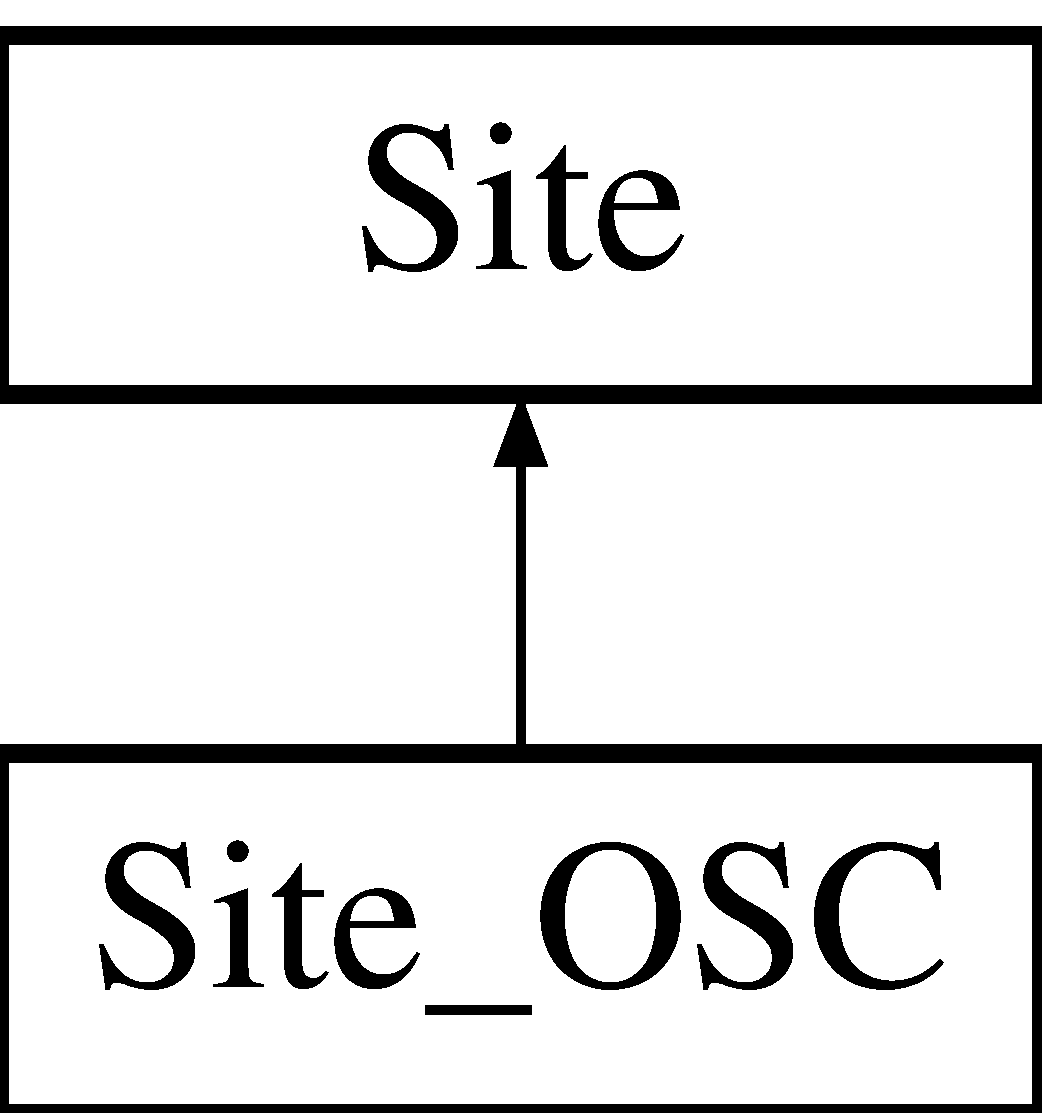
\includegraphics[height=2.000000cm]{class_site}
\end{center}
\end{figure}
\subsection*{Public Member Functions}
\begin{DoxyCompactItemize}
\item 
\mbox{\Hypertarget{class_site_a81f7ae39aaa7a981a6871c4816ee5562}\label{class_site_a81f7ae39aaa7a981a6871c4816ee5562}} 
virtual \hyperlink{class_site_a81f7ae39aaa7a981a6871c4816ee5562}{$\sim$\+Site} ()
\begin{DoxyCompactList}\small\item\em Default virtual destructor needed by the base class. \end{DoxyCompactList}\item 
\mbox{\Hypertarget{class_site_a4119f95c45d57d6edf419169dea993f4}\label{class_site_a4119f95c45d57d6edf419169dea993f4}} 
\hyperlink{class_site_a4119f95c45d57d6edf419169dea993f4}{Site} ()
\begin{DoxyCompactList}\small\item\em Default constructor that creates an empty \hyperlink{class_object}{Object} object. \end{DoxyCompactList}\item 
void \hyperlink{class_site_a46ff077954e39046b493ee1ea57a9c93}{clear\+Occupancy} ()
\begin{DoxyCompactList}\small\item\em Clears the occupancy of the site. \end{DoxyCompactList}\item 
\mbox{\Hypertarget{class_site_aecb14e440914b4d3d4aa7294419791e2}\label{class_site_aecb14e440914b4d3d4aa7294419791e2}} 
\hyperlink{class_object}{Object} $\ast$ \hyperlink{class_site_aecb14e440914b4d3d4aa7294419791e2}{get\+Object\+Ptr} () const
\begin{DoxyCompactList}\small\item\em Gets the pointer to the \hyperlink{class_object}{Object} object that occupies the site. \end{DoxyCompactList}\item 
bool \hyperlink{class_site_a30991b768ded0bb441c5bb54a789160a}{is\+Occupied} () const
\begin{DoxyCompactList}\small\item\em Checks whether the site is occupied or not. \end{DoxyCompactList}\item 
void \hyperlink{class_site_a9a0d305451d7732dbb193e7fd2f502ca}{set\+Object\+Ptr} (\hyperlink{class_object}{Object} $\ast$input\+\_\+ptr)
\begin{DoxyCompactList}\small\item\em Sets the pointer to the occupying \hyperlink{class_object}{Object}. \end{DoxyCompactList}\item 
\mbox{\Hypertarget{class_site_ab85bec20c3a6067a7dca659221d57d25}\label{class_site_ab85bec20c3a6067a7dca659221d57d25}} 
void \hyperlink{class_site_ab85bec20c3a6067a7dca659221d57d25}{set\+Occupied} ()
\begin{DoxyCompactList}\small\item\em Sets the site to an occupied state. \end{DoxyCompactList}\end{DoxyCompactItemize}


\subsection{Detailed Description}
This base class contains the basic properties of a lattice site and the functions needed to interact with it. 

This base class is designed to be used by the \hyperlink{class_lattice}{Lattice} class to construct a lattice that will be used by a K\+MC simulation. This class is designed to for sites to have single occupancy, but multiple occupancy could potentially be implemented in a derived class. \begin{DoxyCopyright}{Copyright}
M\+IT License. For more information, see the L\+I\+C\+E\+N\+SE file that accompanies this software package. 
\end{DoxyCopyright}
\begin{DoxyAuthor}{Author}
Michael C. Heiber 
\end{DoxyAuthor}
\begin{DoxyDate}{Date}
2017 
\end{DoxyDate}


\subsection{Member Function Documentation}
\mbox{\Hypertarget{class_site_a46ff077954e39046b493ee1ea57a9c93}\label{class_site_a46ff077954e39046b493ee1ea57a9c93}} 
\index{Site@{Site}!clear\+Occupancy@{clear\+Occupancy}}
\index{clear\+Occupancy@{clear\+Occupancy}!Site@{Site}}
\subsubsection{\texorpdfstring{clear\+Occupancy()}{clearOccupancy()}}
{\footnotesize\ttfamily void Site\+::clear\+Occupancy (\begin{DoxyParamCaption}{ }\end{DoxyParamCaption})}



Clears the occupancy of the site. 

This function also sets the \hyperlink{class_object}{Object} pointer to nullptr. \mbox{\Hypertarget{class_site_a30991b768ded0bb441c5bb54a789160a}\label{class_site_a30991b768ded0bb441c5bb54a789160a}} 
\index{Site@{Site}!is\+Occupied@{is\+Occupied}}
\index{is\+Occupied@{is\+Occupied}!Site@{Site}}
\subsubsection{\texorpdfstring{is\+Occupied()}{isOccupied()}}
{\footnotesize\ttfamily bool Site\+::is\+Occupied (\begin{DoxyParamCaption}{ }\end{DoxyParamCaption}) const}



Checks whether the site is occupied or not. 

\begin{DoxyReturn}{Returns}
true if the site occupied. 

false if the site is unoccupied. 
\end{DoxyReturn}
\mbox{\Hypertarget{class_site_a9a0d305451d7732dbb193e7fd2f502ca}\label{class_site_a9a0d305451d7732dbb193e7fd2f502ca}} 
\index{Site@{Site}!set\+Object\+Ptr@{set\+Object\+Ptr}}
\index{set\+Object\+Ptr@{set\+Object\+Ptr}!Site@{Site}}
\subsubsection{\texorpdfstring{set\+Object\+Ptr()}{setObjectPtr()}}
{\footnotesize\ttfamily void Site\+::set\+Object\+Ptr (\begin{DoxyParamCaption}\item[{\hyperlink{class_object}{Object} $\ast$}]{input\+\_\+ptr }\end{DoxyParamCaption})}



Sets the pointer to the occupying \hyperlink{class_object}{Object}. 

Also sets the site to an occupied state. 

The documentation for this class was generated from the following files\+:\begin{DoxyCompactItemize}
\item 
K\+M\+C\+\_\+\+Lattice/Site.\+h\item 
K\+M\+C\+\_\+\+Lattice/Site.\+cpp\end{DoxyCompactItemize}

\hypertarget{class_site___o_s_c}{}\section{Site\+\_\+\+O\+SC Class Reference}
\label{class_site___o_s_c}\index{Site\+\_\+\+O\+SC@{Site\+\_\+\+O\+SC}}
Inheritance diagram for Site\+\_\+\+O\+SC\+:\begin{figure}[H]
\begin{center}
\leavevmode
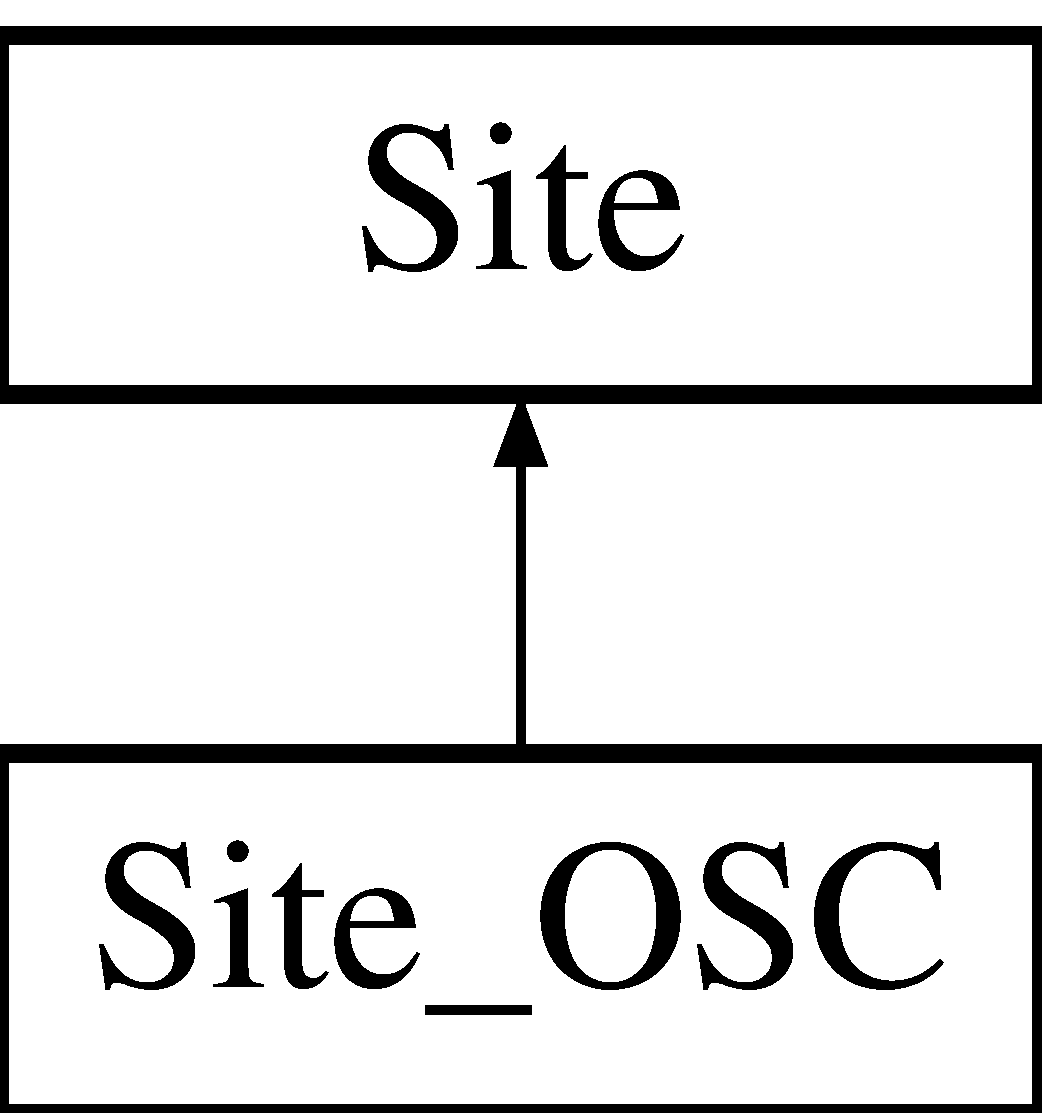
\includegraphics[height=2.000000cm]{class_site___o_s_c}
\end{center}
\end{figure}
\subsection*{Public Member Functions}
\begin{DoxyCompactItemize}
\item 
\mbox{\Hypertarget{class_site___o_s_c_a59db8200675439b98f42d3c35310fe68}\label{class_site___o_s_c_a59db8200675439b98f42d3c35310fe68}} 
double {\bfseries get\+Energy} () const
\item 
\mbox{\Hypertarget{class_site___o_s_c_a704a0a9fe1bab69db8343f5225d5888e}\label{class_site___o_s_c_a704a0a9fe1bab69db8343f5225d5888e}} 
short {\bfseries get\+Type} () const
\item 
\mbox{\Hypertarget{class_site___o_s_c_ac7751de2f821aa8562793f8636027313}\label{class_site___o_s_c_ac7751de2f821aa8562793f8636027313}} 
void {\bfseries set\+Energy} (const double energy)
\item 
\mbox{\Hypertarget{class_site___o_s_c_a22e8a3f697fa69d6a382e91c78a181b3}\label{class_site___o_s_c_a22e8a3f697fa69d6a382e91c78a181b3}} 
void {\bfseries set\+Energy\+It} (const std\+::vector$<$ double $>$\+::iterator it)
\item 
\mbox{\Hypertarget{class_site___o_s_c_a47f7ed4c7e916e01bd5cfc37599babb6}\label{class_site___o_s_c_a47f7ed4c7e916e01bd5cfc37599babb6}} 
void {\bfseries set\+Type} (const short site\+\_\+type)
\end{DoxyCompactItemize}


The documentation for this class was generated from the following file\+:\begin{DoxyCompactItemize}
\item 
O\+S\+C\+\_\+\+Sim.\+h\end{DoxyCompactItemize}

%--- End generated contents ---

% Index
\backmatter
\newpage
\phantomsection
\clearemptydoublepage
\addcontentsline{toc}{chapter}{Index}
\printindex

\end{document}
